\chapter{Anomalous Quartic Gauge Coupling Measurement} % (fold)
\label{cha:anomalous_quartic_gauge_coupling_measurement}
At the LHC, VBS is characterized by presence of two gauge bosons in association with two forward jets with large rapidity separation and a large dijet mass. The VBS topology is produced via the EW interaction with increased sensitivity to quartic gauge couplings. Figure~\ref{fig:feynman} shows the Feynman diagrams involving quartic vertices. An excess of events with respect to SM predictions could indicate the presence of anomalous Quartic Gauge Couplings (aQGCs)~\cite{aqgc_operators} or the existence of new resonances. 

\begin{figure*}[!htbp]
\centering
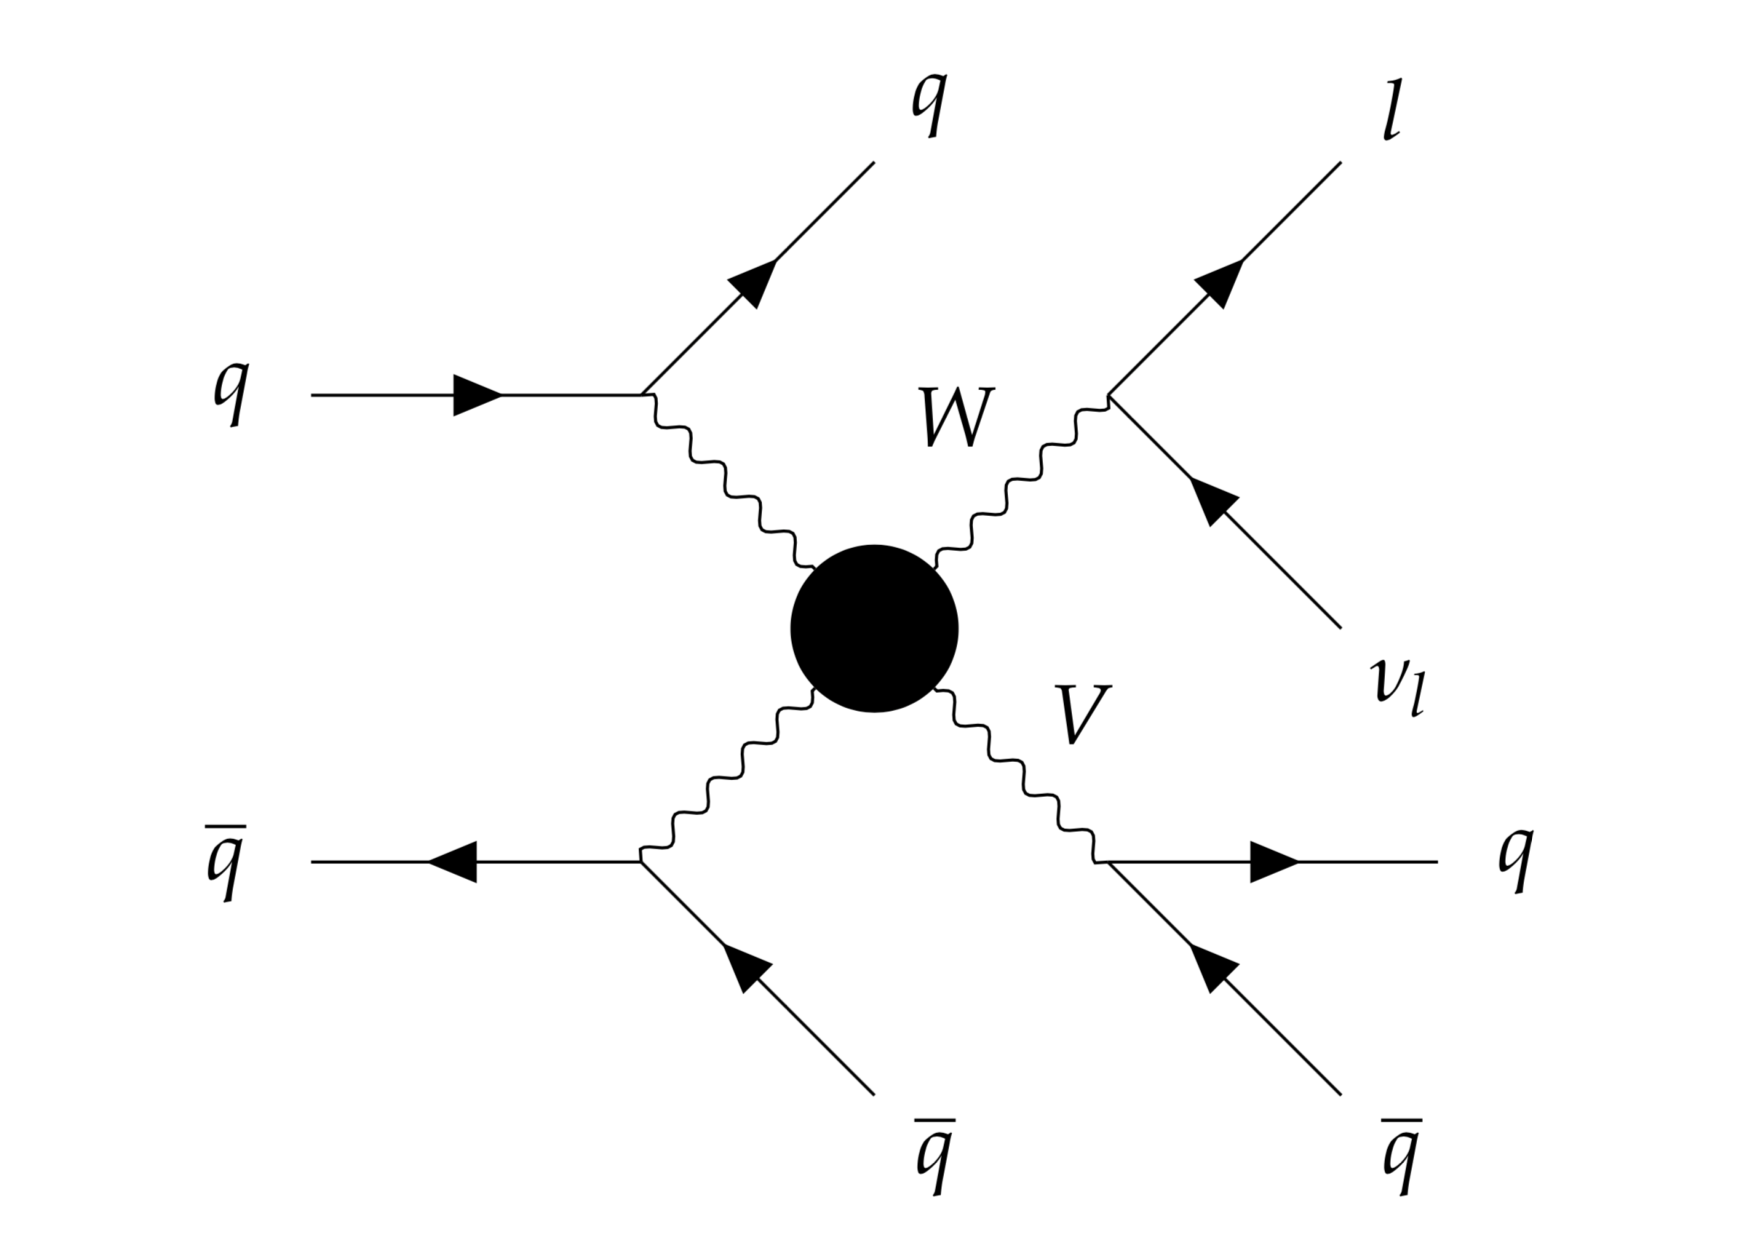
\includegraphics[width=0.45\textwidth]{Pictures/FeynmanDiagram_WV.pdf}
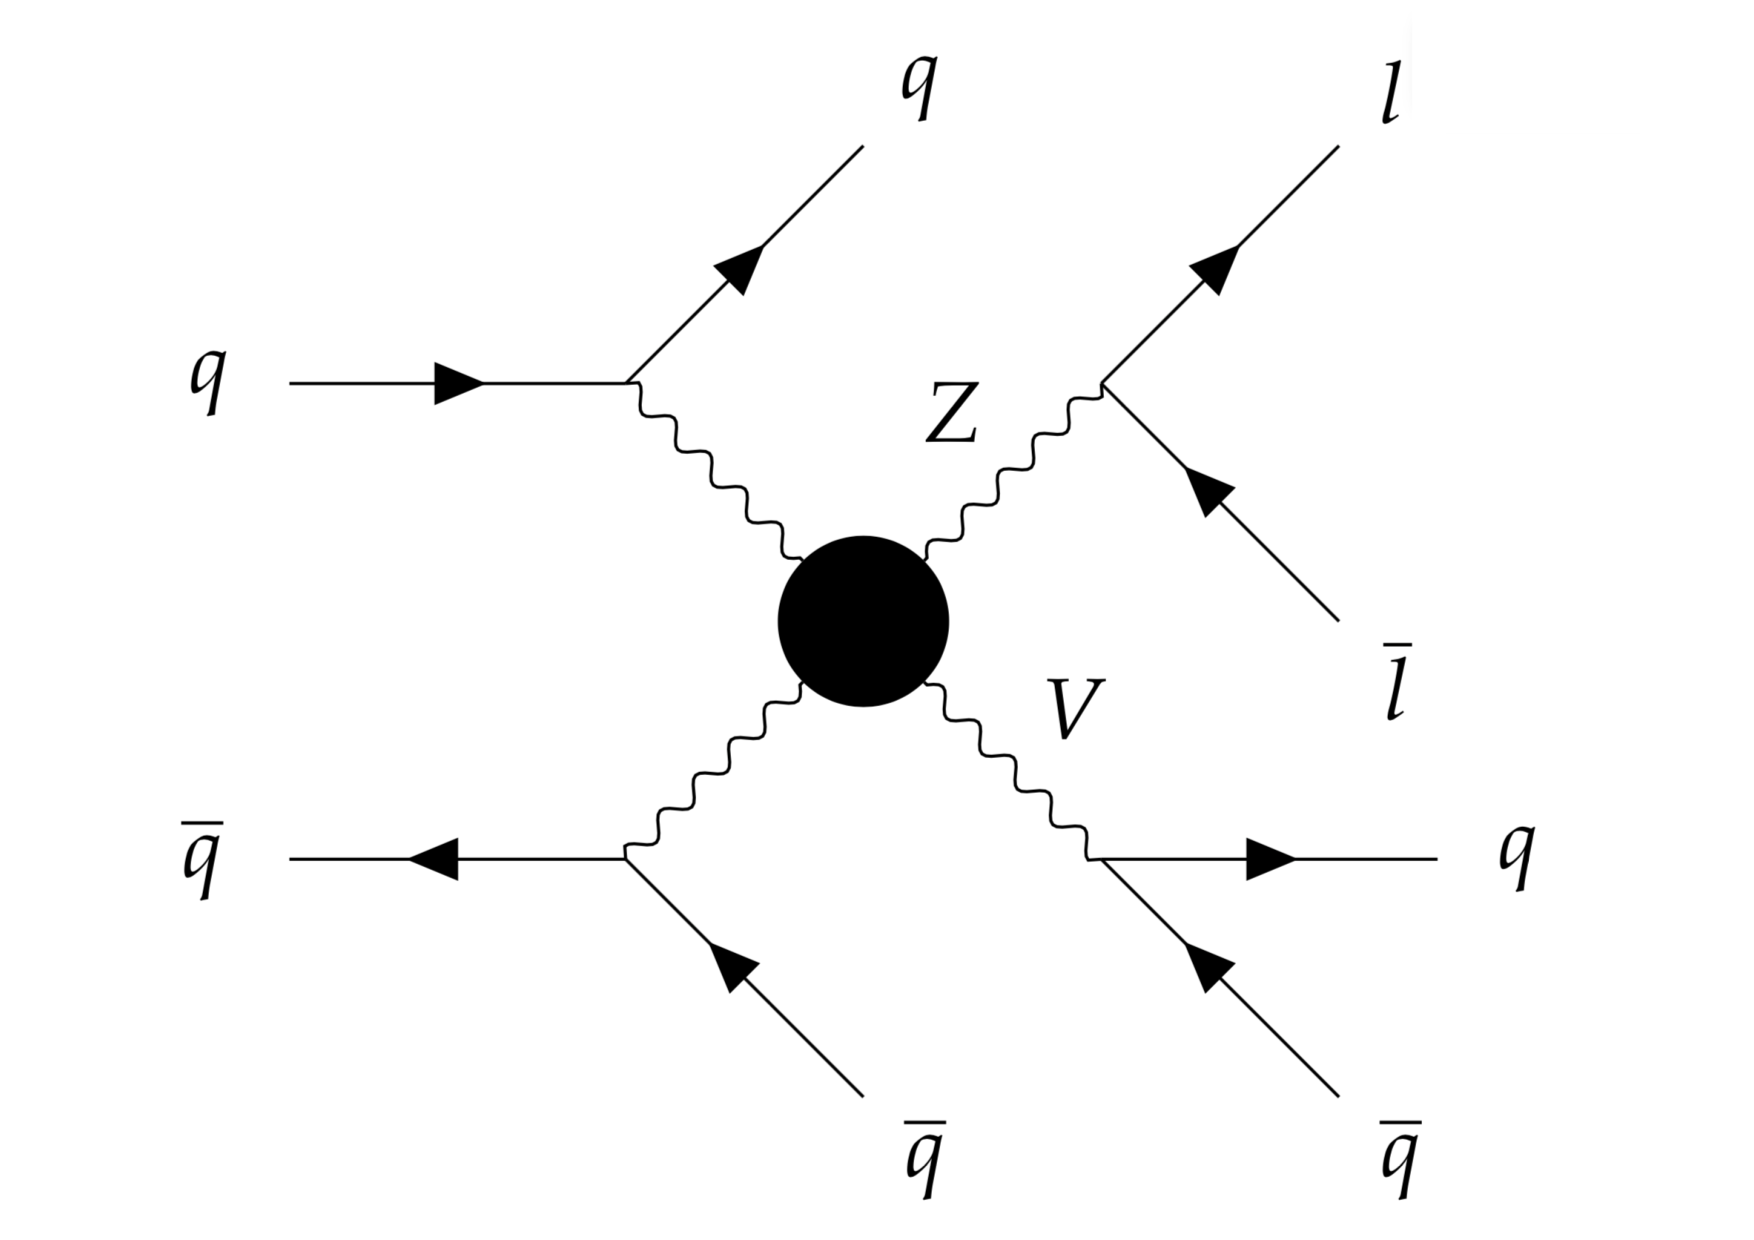
\includegraphics[width=0.45\textwidth]{Pictures/FeynmanDiagram_ZV.pdf}
\caption{VBS Feynman diagrams contributing to the EW induced production of events containing a hadronically decaying gauge boson ($V$), a $\PW$ (left) or $\PZ$ (right) boson decaying to leptons (electrons or muons), and two forward jets. New physics in the EW sector can modify the quartic gauge coupling.}
\label{fig:feynman}
\end{figure*}

The main goal of this analysis is to search for the presence of aQGCs in candidate events containing a hadronically decaying gauge boson ($V$) produced with large transverse momentum $\pt$, a $\PW$ or $\PZ$ boson decaying to leptons (electrons or muons), and two forward jets. This final state benefits from a higher branching ratio of the $V$ decay compared to previous searches at the LHC for aQGCs in VBS involving only leptonic boson decays~\cite{Sirunyan:2017ret, ATLAS_ssWW, CMS_ssWW, Aaboud:2016ffv,Aad:2016ett, Sirunyan:2017fvv, Khachatryan:2016mud, Khachatryan:2017jub, Khachatryan:2016vif,Aaboud:2017pds}. The ATLAS collaboration reported limits on aQGCs in VBS using the $\PW V$ final state, where $\PW$ decays to leptons, in proton-proton (pp) collisions at $\sqrt{s}=8\TeV$~\cite{Aaboud2017}. 

Extended Higgs sectors with additional SU(2) isotriplet scalar give rise to charged Higgs bosons with couplings to $\PW$ and $\PZ$ bosons at the tree level~\cite{Englert2013a}. In particular, the Georgi-Machacek (GM)~\cite{GEORGI1985463} model, with both real and complex triplets,  preserves the tree level custodial symmetry. In this model, singly and doubly charged Higgs bosons are produced via vector boson fusion (VBF) and decay to $\PW$ and $\PZ$ bosons, and same-sign $\PW$ boson pairs, respectively. The ATLAS and CMS Collaborations performed searches for charged Higgs bosons in these topologies and set constraints on the GM model~\cite{Sirunyan:2017ret,Sirunyan:2017sbn,PhysRevLett.114.231801}.

This chapter presents a study of VBS in $\PW\PW$, $\PW\PZ$, and $\PZ\PZ$ final states using pp collisions at $\sqrt{s}=13\TeV$. The data sample corresponds to an integrated luminosity of $35.9 \pm 0.9\fbinv$ collected with the CMS detector~\cite{Chatrchyan:2008zzk} at the CERN LHC in 2016. 

% \section{Generation Details of Signal Sample}
% \label{sec:MCsampleGeneration}
% \subsection{Madgraph setup and parameters}

% \begin{sloppypar}
% Madgraph cards are located here: \url{https://github.com/cms-sw/genproductions/tree/pre2017/bin/MadGraph5_aMCatNLO/cards/production/13TeV/VBS/VVjj_semileptonic}
% \end{sloppypar}

% The gridpacks for signal can be found here:

% \begin{sloppypar}
% \url{/cvmfs/cms.cern.ch/phys\_generator/gridpacks/slc6\_amd64\_gcc481/13TeV/madgraph/V5\_2.4.2/AnomalousCouplingsSMP}
% \end{sloppypar}

% \subsection{How samples are generated?}
% We generated our signal using Madgraph version V5\_2.4.2. The main setting used different from default run card are 
% \begin{itemize}
%   \item maxjetflavor = 5
%   \item mjj = 100
% \end{itemize}

% \subsubsection{SM signal sample generation}
% Signal sample was generated with pure electroweak vertex with option "QED=4 and QCD=0". Below you can see the proc card information. 

% \begin{verbatim}
% set group_subprocesses Auto
% set ignore_six_quark_processes False
% set loop_optimized_output True
% set complex_mass_scheme False
% import model sm-ckm_no_b_mass
% define p = g u c d s b u~ c~ d~ s~ b~
% define j = p 
% define l+ = e+ mu+ ta+
% define l- = e- mu- ta-
% define vl = ve vm vt
% define vl~ = ve~ vm~ vt~
% generate p p > w+ w- j j QED=4 QCD=0 
% output WPlepWMhadJJ_EWK_LO_SM_mjj100_pTj10 --nojpeg
% \end{verbatim}

% \subsubsection{aQGC signal sample generation}
% aQGC sample generated with effective field theory with dimension eight effective operators assuming that the recently observed Higgs boson belongs to a SU(2)$_{L}$ doublet, with the method proposed by Eboli~\cite{Belyaev:1998ih,aqgc_operators,Eboli:2000ad,Eboli:2003nq}
% \begin{verbatim}
% set group_subprocesses Auto
% set ignore_six_quark_processes False
% set complex_mass_scheme False
% import model SM_LS_LM_LT_UFO
% define p = g u c d s u~ c~ d~ s~ 
% define j = g u c d s u~ c~ d~ s~ b b~
% define l+ = e+ mu+ ta+
% define l- = e- mu- ta-
% define vl = ve vm vt
% define vl~ = ve~ vm~ vt~
% generate p p > w- w+ j j QED=4 QCD=0 NP=1
% output aQGC_WMhadWPlepJJ_EWK_LO_NPle1_mjj100pt10 --nojpeg
% \end{verbatim}
% To generate aQGC sample we used option {\bf NP=1}. This option forces madgraph to generate sample having SM, aQGC, and interference diagrams.
% Also, we can not decay w-boson here with madgraph because of the limitation of the Madgraph. The issue is that madgraph uses only final state in order to identify which matrix-element to use but it can not able to distinguish which of the jets are coming from the $W^+$. This is the source of error. Here, you can follow the discussion with authors:
% \begin{sloppypar}
%   \url{https://bugs.launchpad.net/mg5amcnlo/+bug/1633803}
% \end{sloppypar}
% Used model can be found at generator repository of models: 
% \begin{sloppypar}
% https://cms-project-generators.web.cern.ch/cms-project-generators/ 
% \end{sloppypar}

% \subsection{Comparison of SM and aQGC distribution}

% \begin{figure}[!htbp]
%   \centering
%   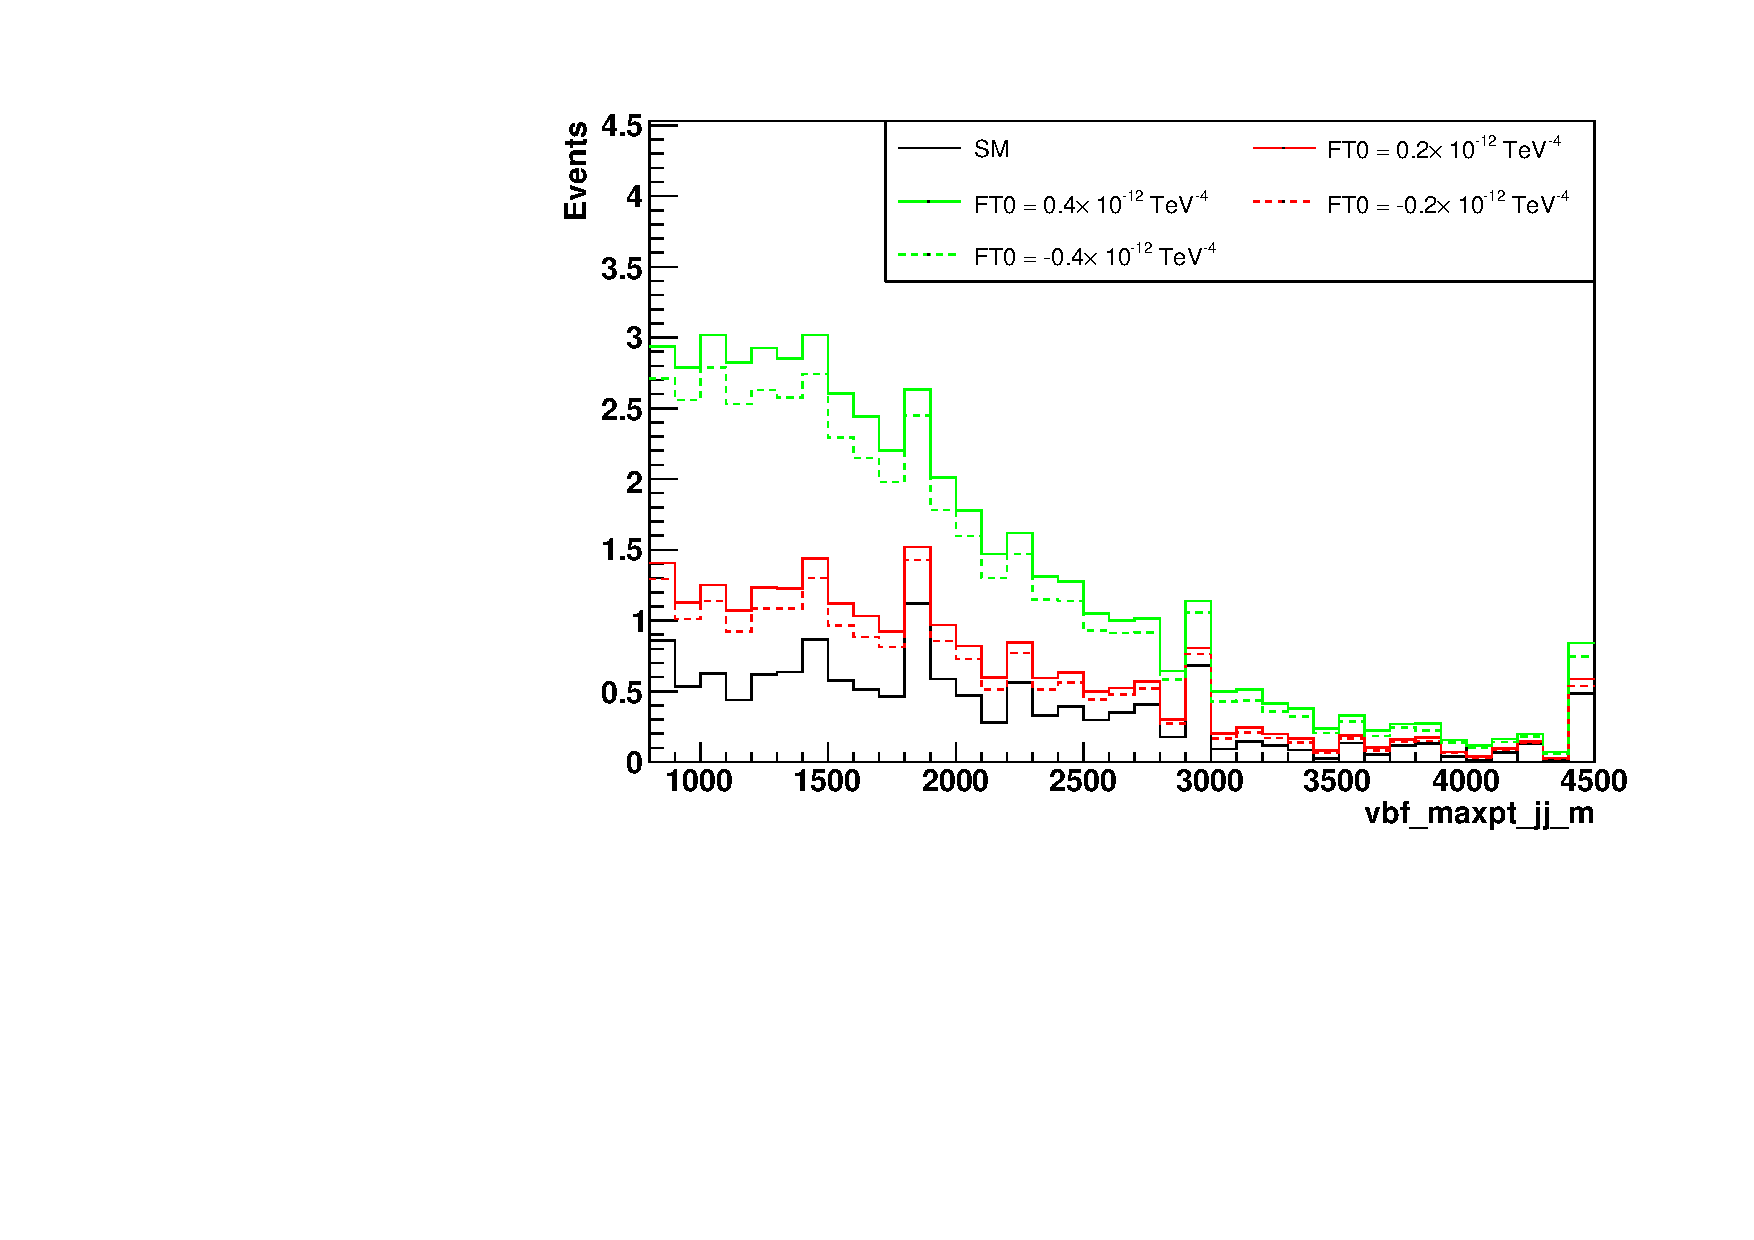
\includegraphics[width=0.45\textwidth]{Plots/aQGC_kinematics/vbf_maxpt_jj_m_FT0.pdf}%
%   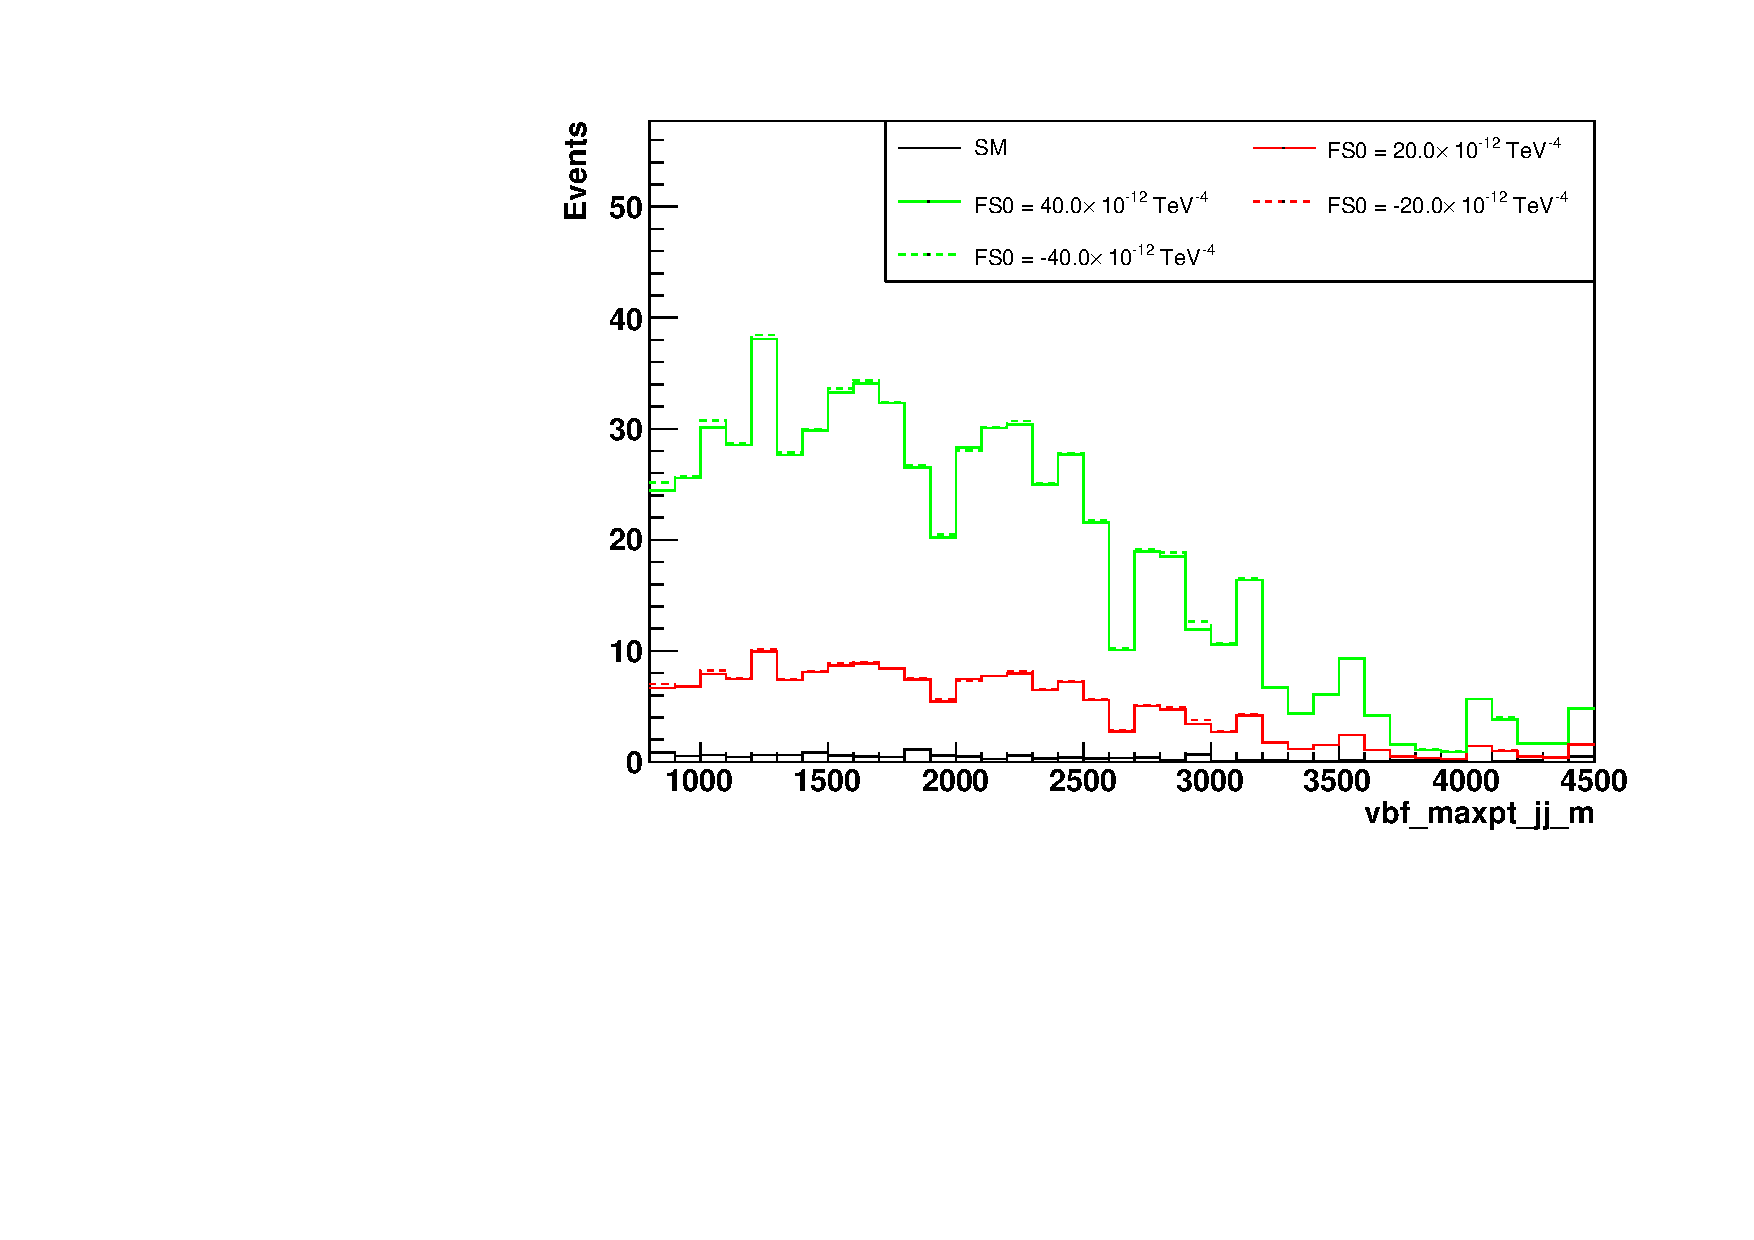
\includegraphics[width=0.45\textwidth]{Plots/aQGC_kinematics/vbf_maxpt_jj_m_FS0.pdf}\\
%   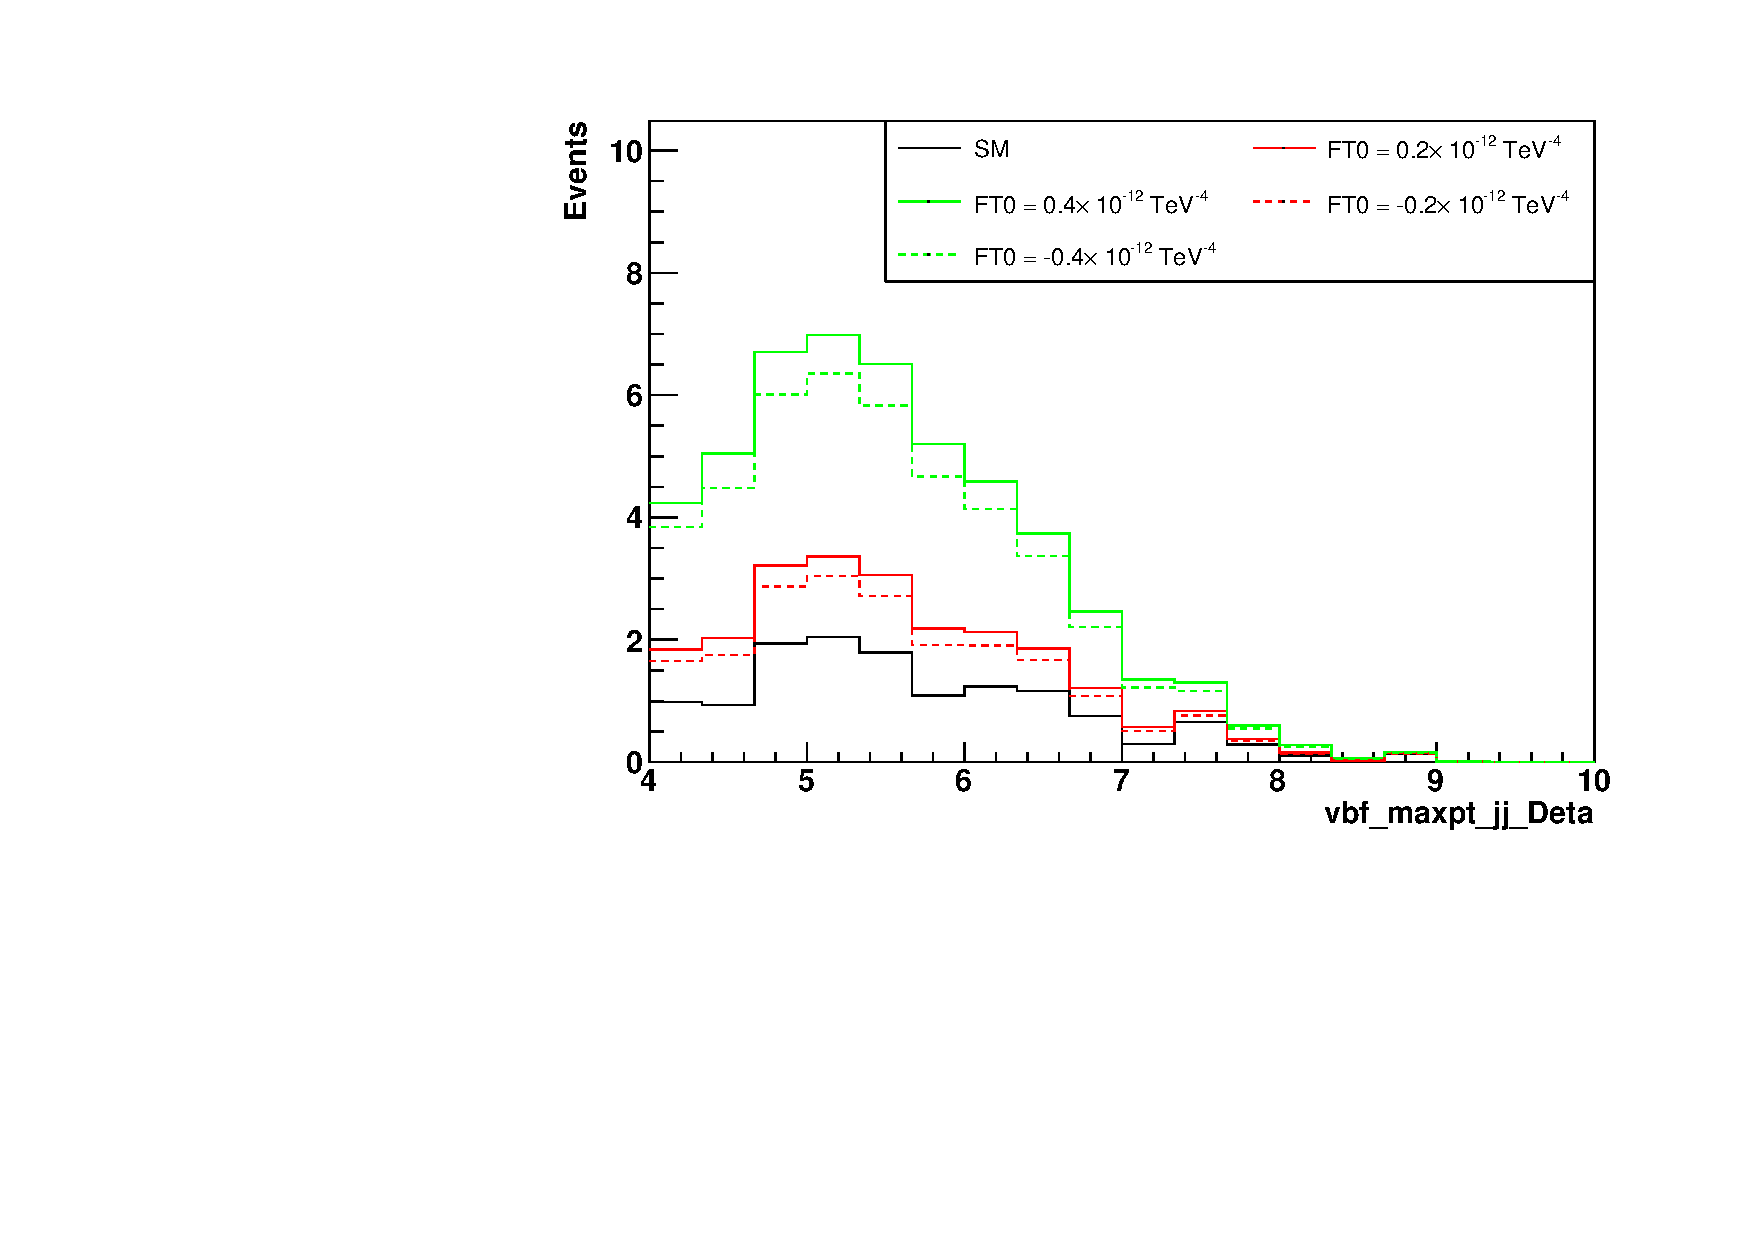
\includegraphics[width=0.45\textwidth]{Plots/aQGC_kinematics/vbf_maxpt_jj_Deta_FT0.pdf}%
%   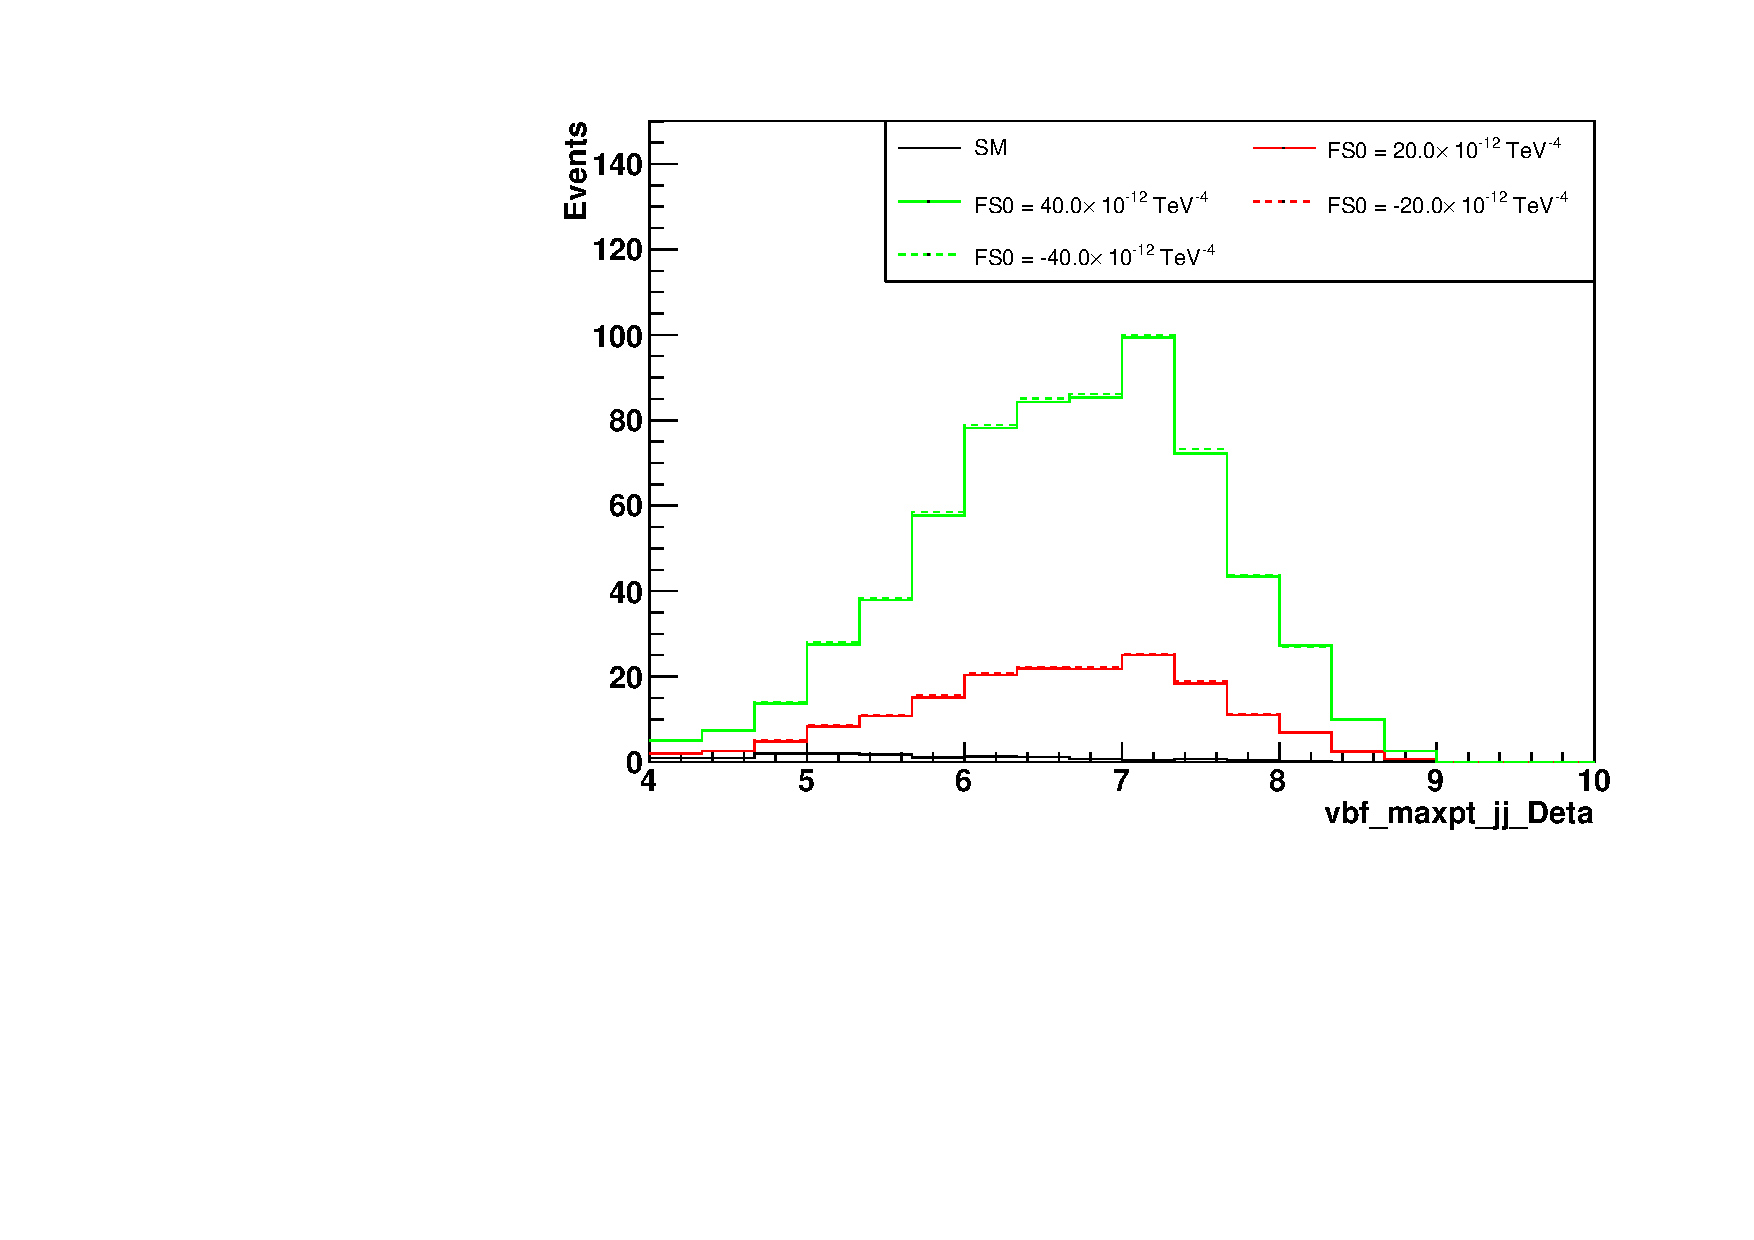
\includegraphics[width=0.45\textwidth]{Plots/aQGC_kinematics/vbf_maxpt_jj_Deta_FS0.pdf}
%   \caption{Top: VBF di-jet invariant mass distribution for aQGC parameter FT0 (left) and FS0 (right). Bottom: VBF di-jet pseudorapidity gap for aQGC parameter FT0 (left) and FS0 (right).}
%   \label{fig:vbf_sm_aqgc}
% \end{figure}

% \begin{figure}[!htbp]
%   % \vspace{-2cm}
%   \centering
%   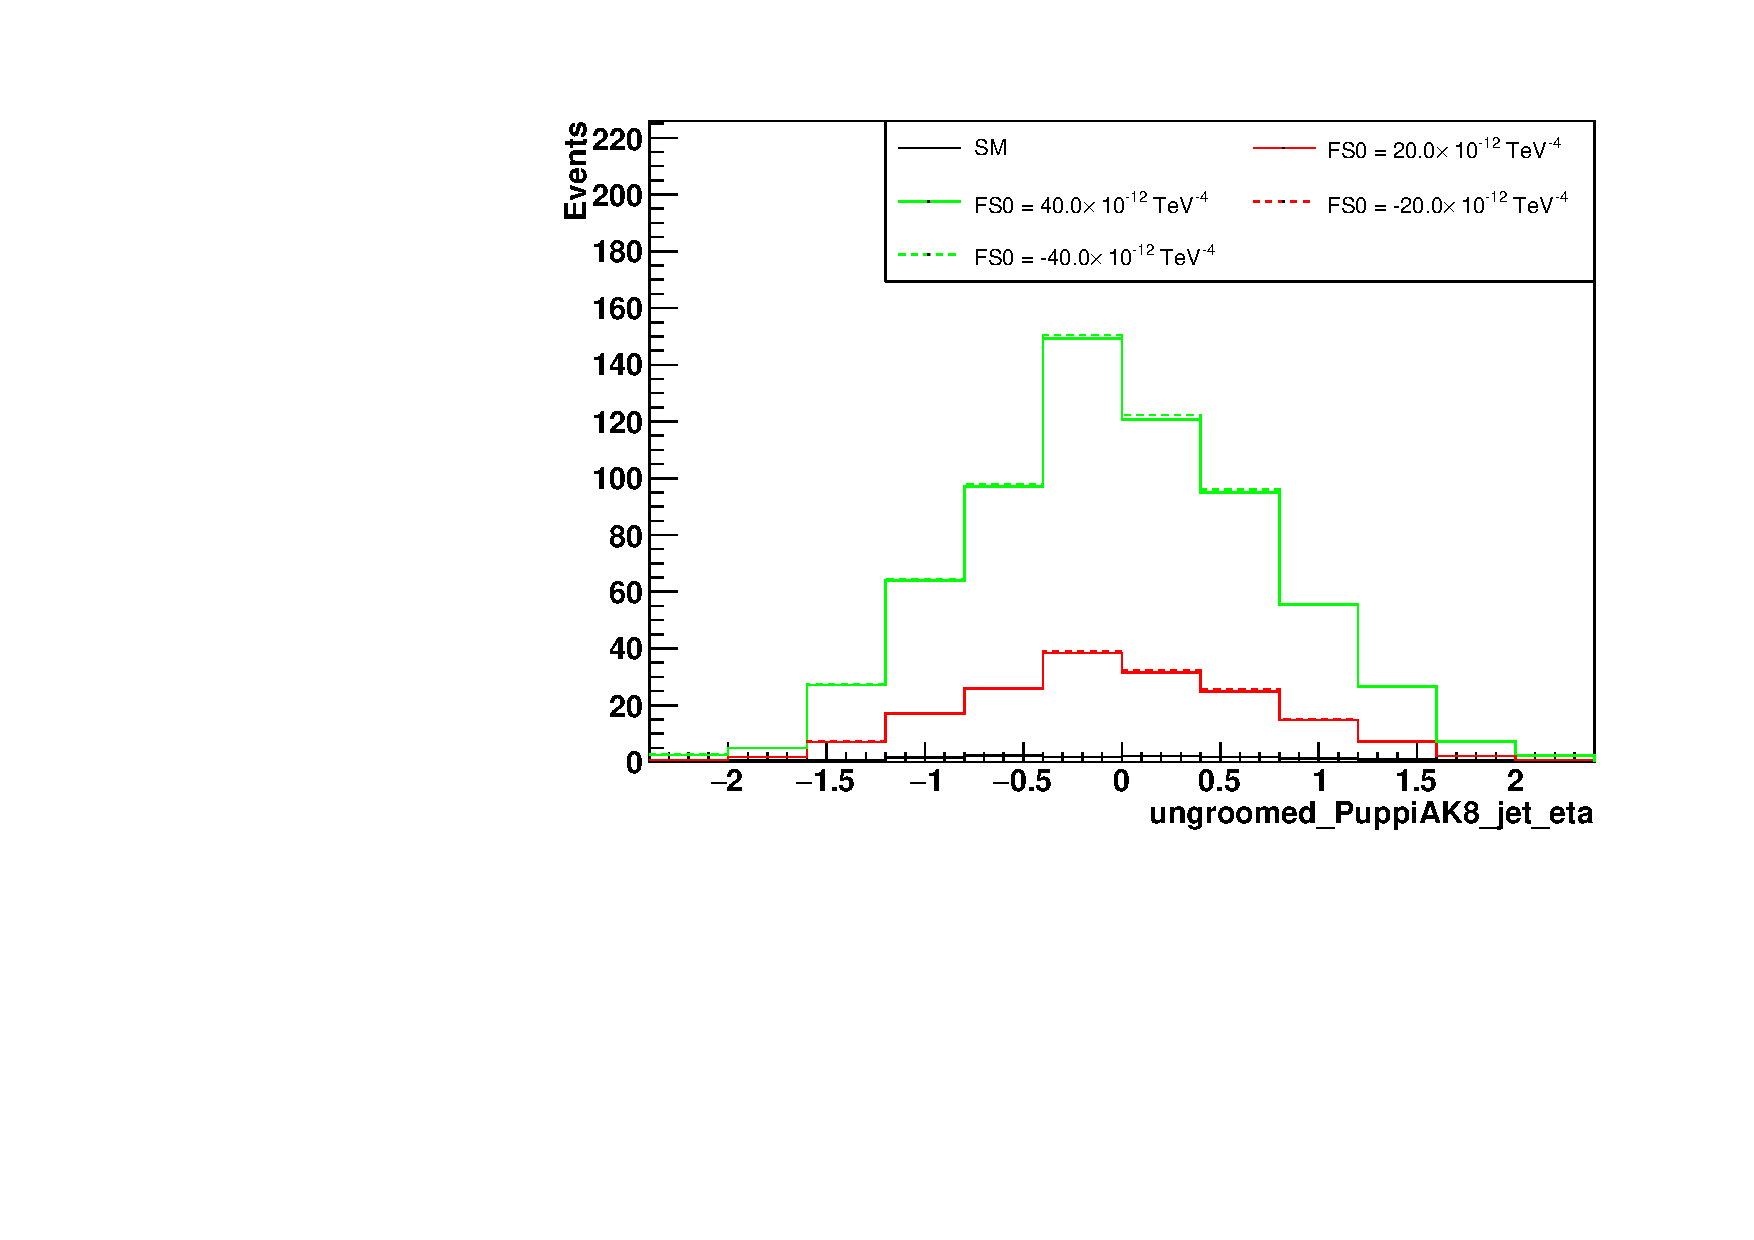
\includegraphics[width=0.40\textwidth]{Plots/aQGC_kinematics/ungroomed_PuppiAK8_jet_eta_FS0.pdf}%
%   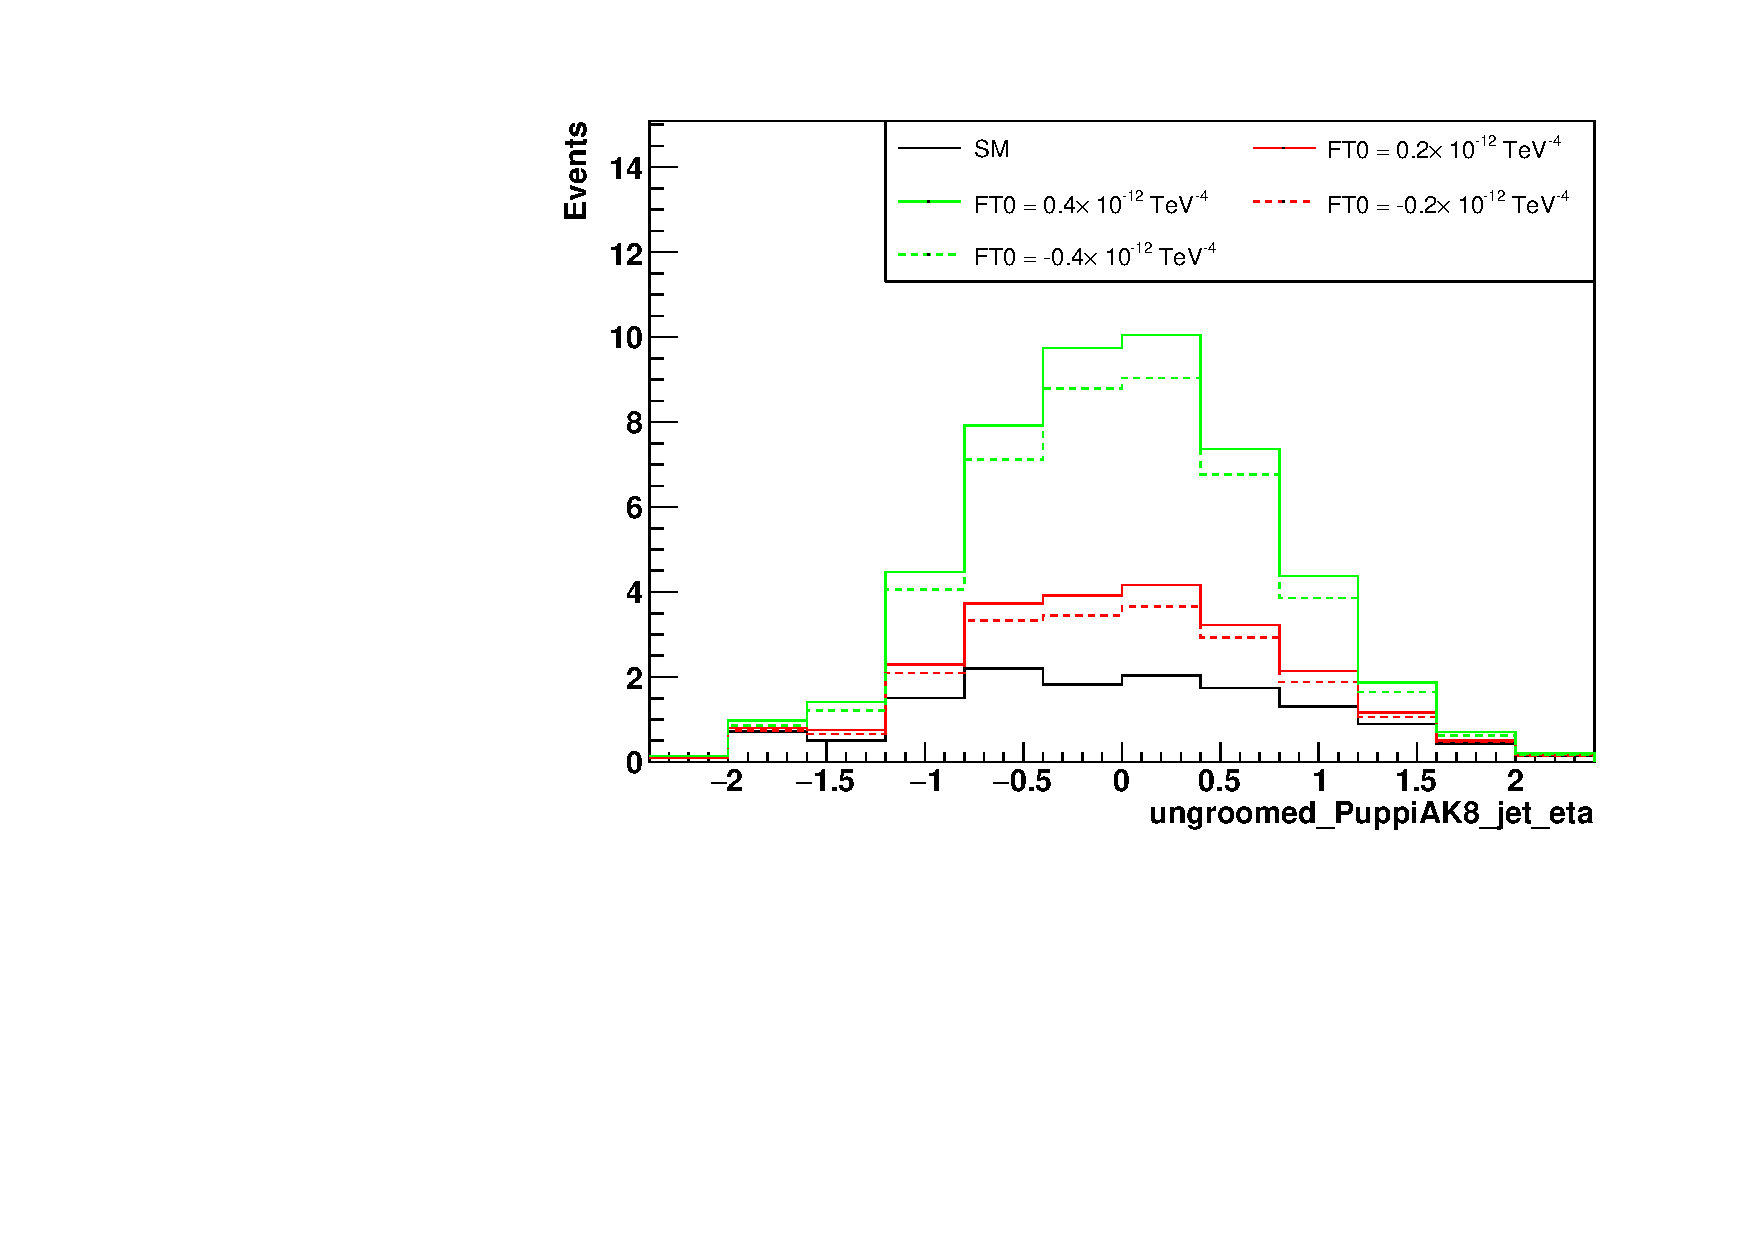
\includegraphics[width=0.40\textwidth]{Plots/aQGC_kinematics/ungroomed_PuppiAK8_jet_eta_FT0.pdf}\\
%   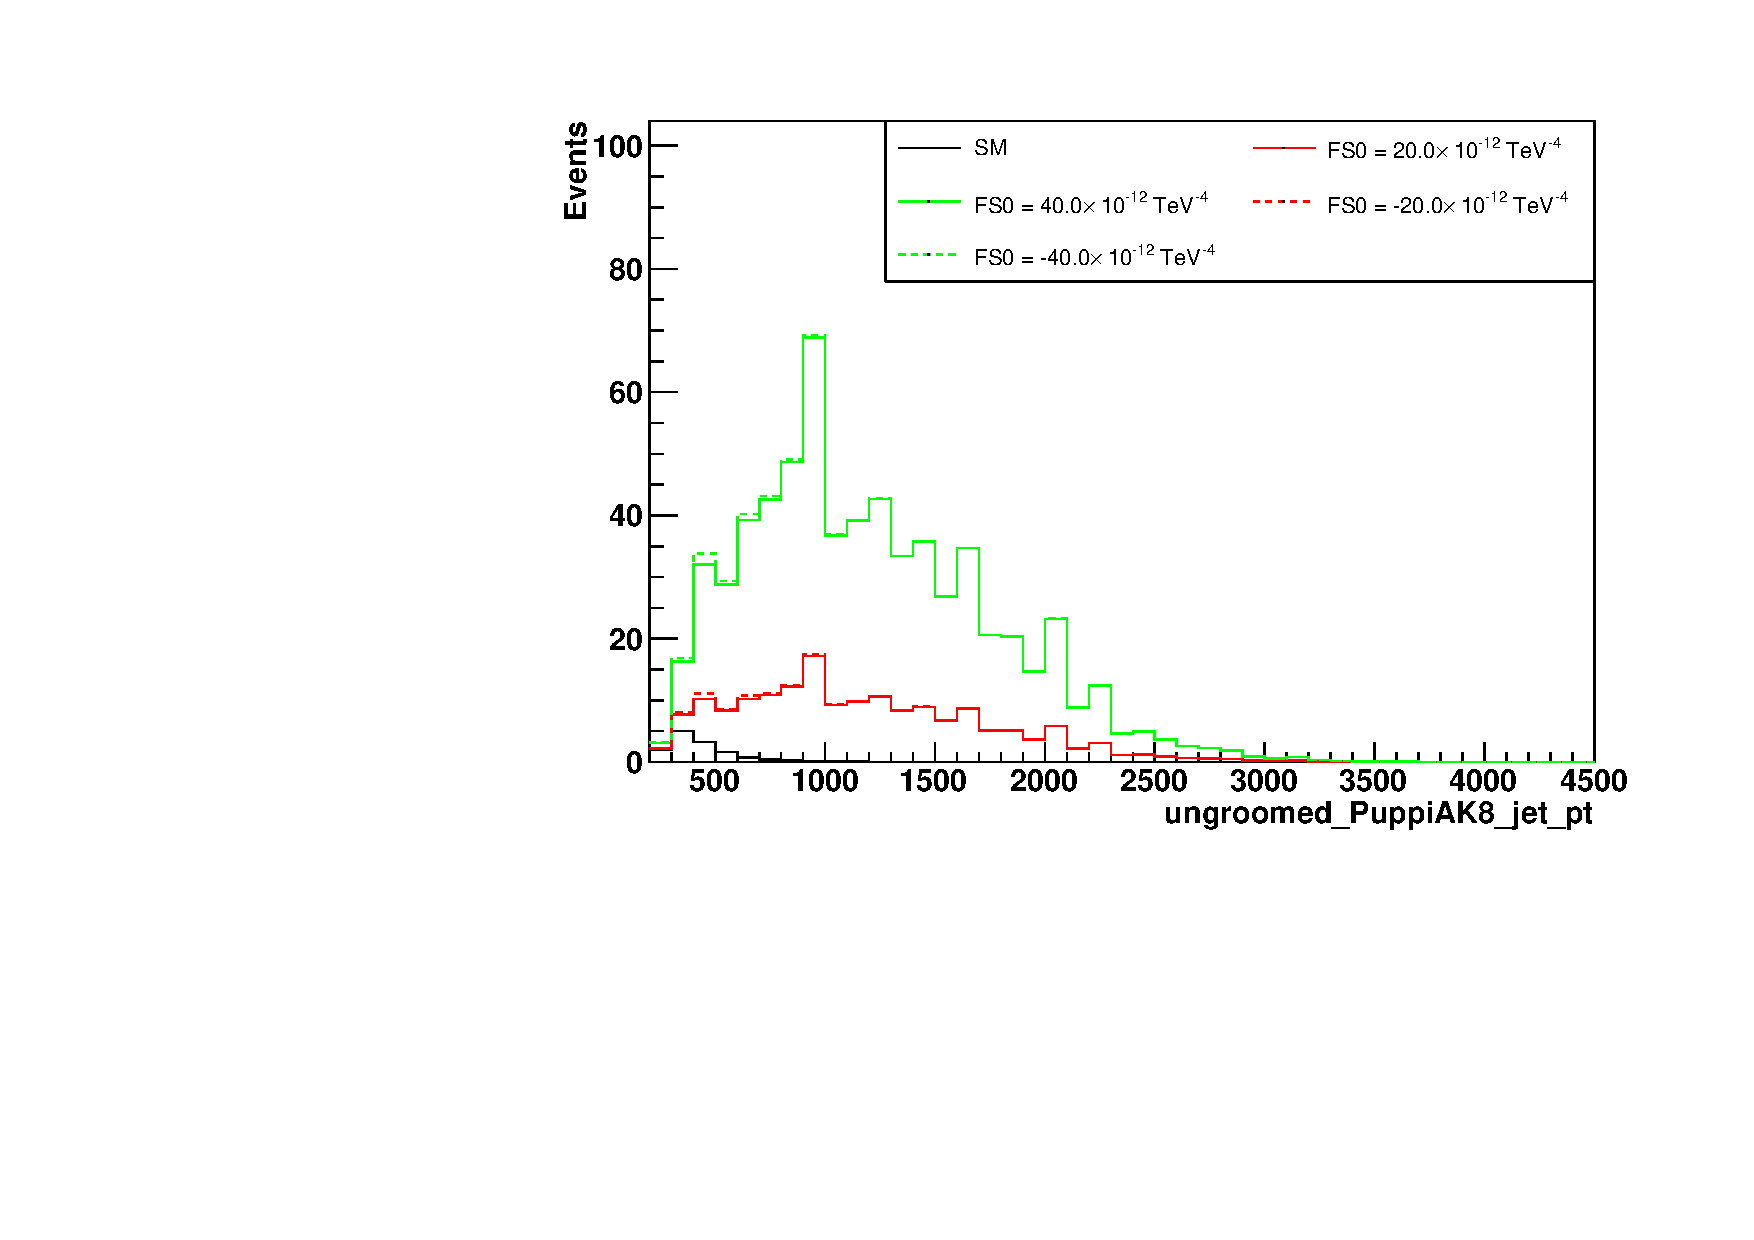
\includegraphics[width=0.40\textwidth]{Plots/aQGC_kinematics/ungroomed_PuppiAK8_jet_pt_FS0.pdf}%
%   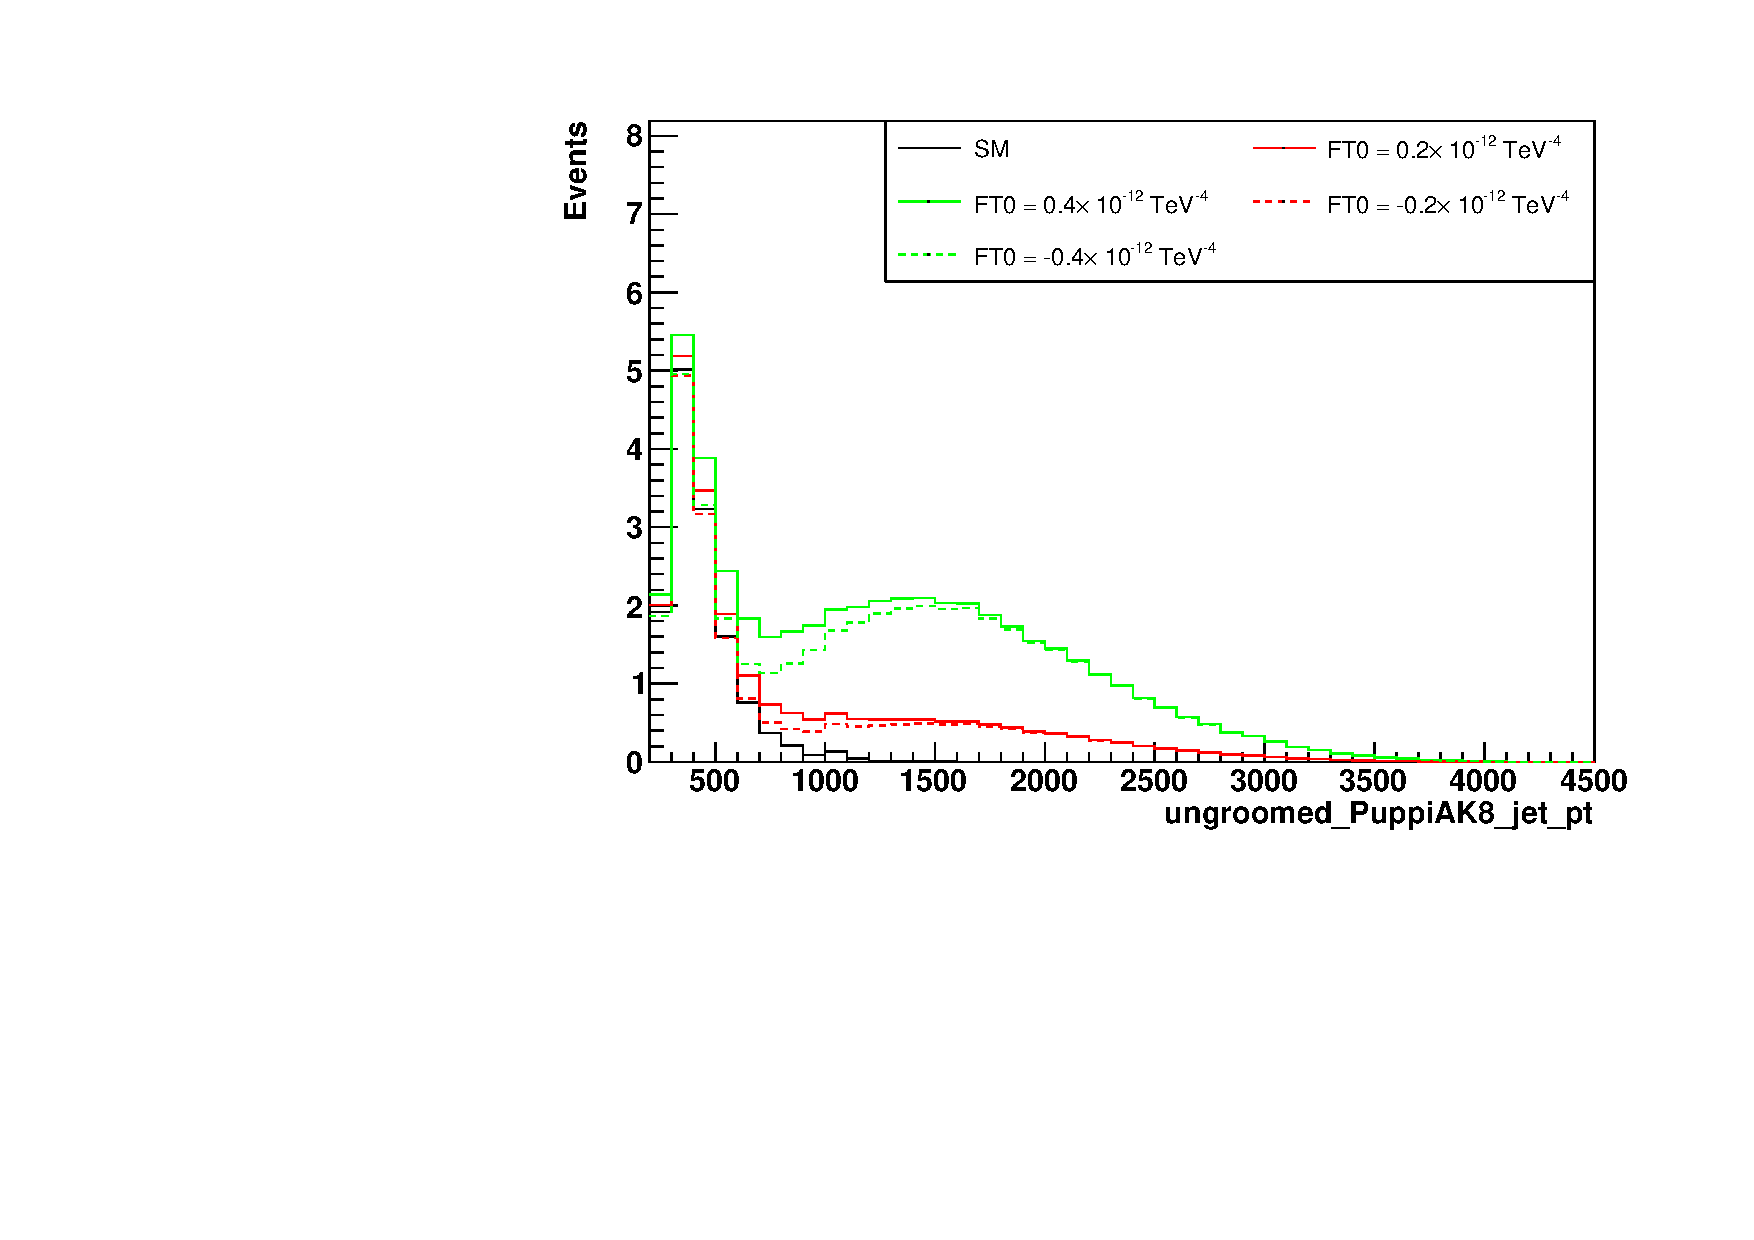
\includegraphics[width=0.40\textwidth]{Plots/aQGC_kinematics/ungroomed_PuppiAK8_jet_pt_FT0.pdf}\\
%   \caption{Top: Fat jet with large radius parameter's pseudo-rapidity  for aQGC parameter FS0 (left) and FT0 (right). Bottom: Fat jet with large radius parameter's transverse momentum distribution shown for aQGC parameter FS0 (left) and FT0 (right).}
%   \label{fig:wjet_sm_aqgc}
% \end{figure}

% \begin{figure}[!htbp]
%   \centering
%   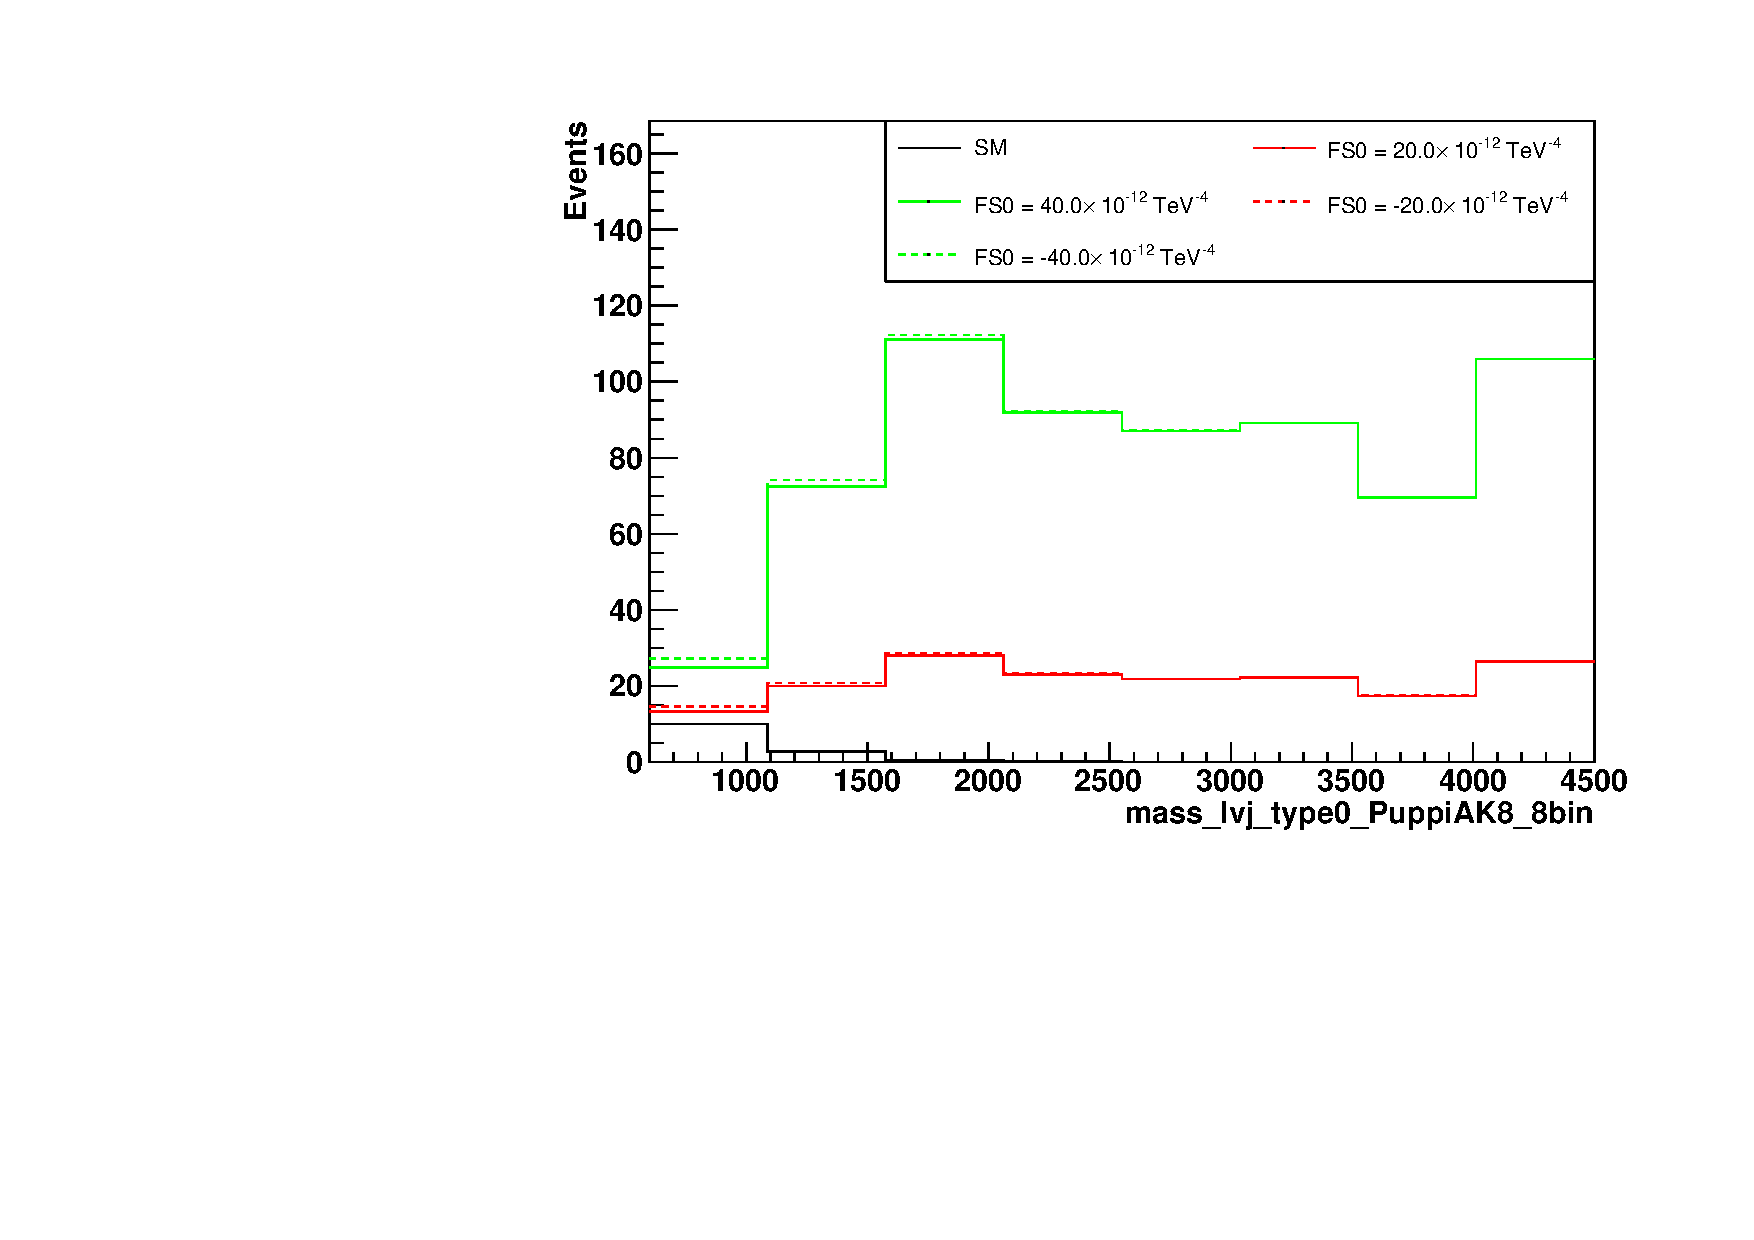
\includegraphics[width=0.40\textwidth]{Plots/aQGC_kinematics/mass_lvj_type0_PuppiAK8_8bin_FS0.pdf}%
%   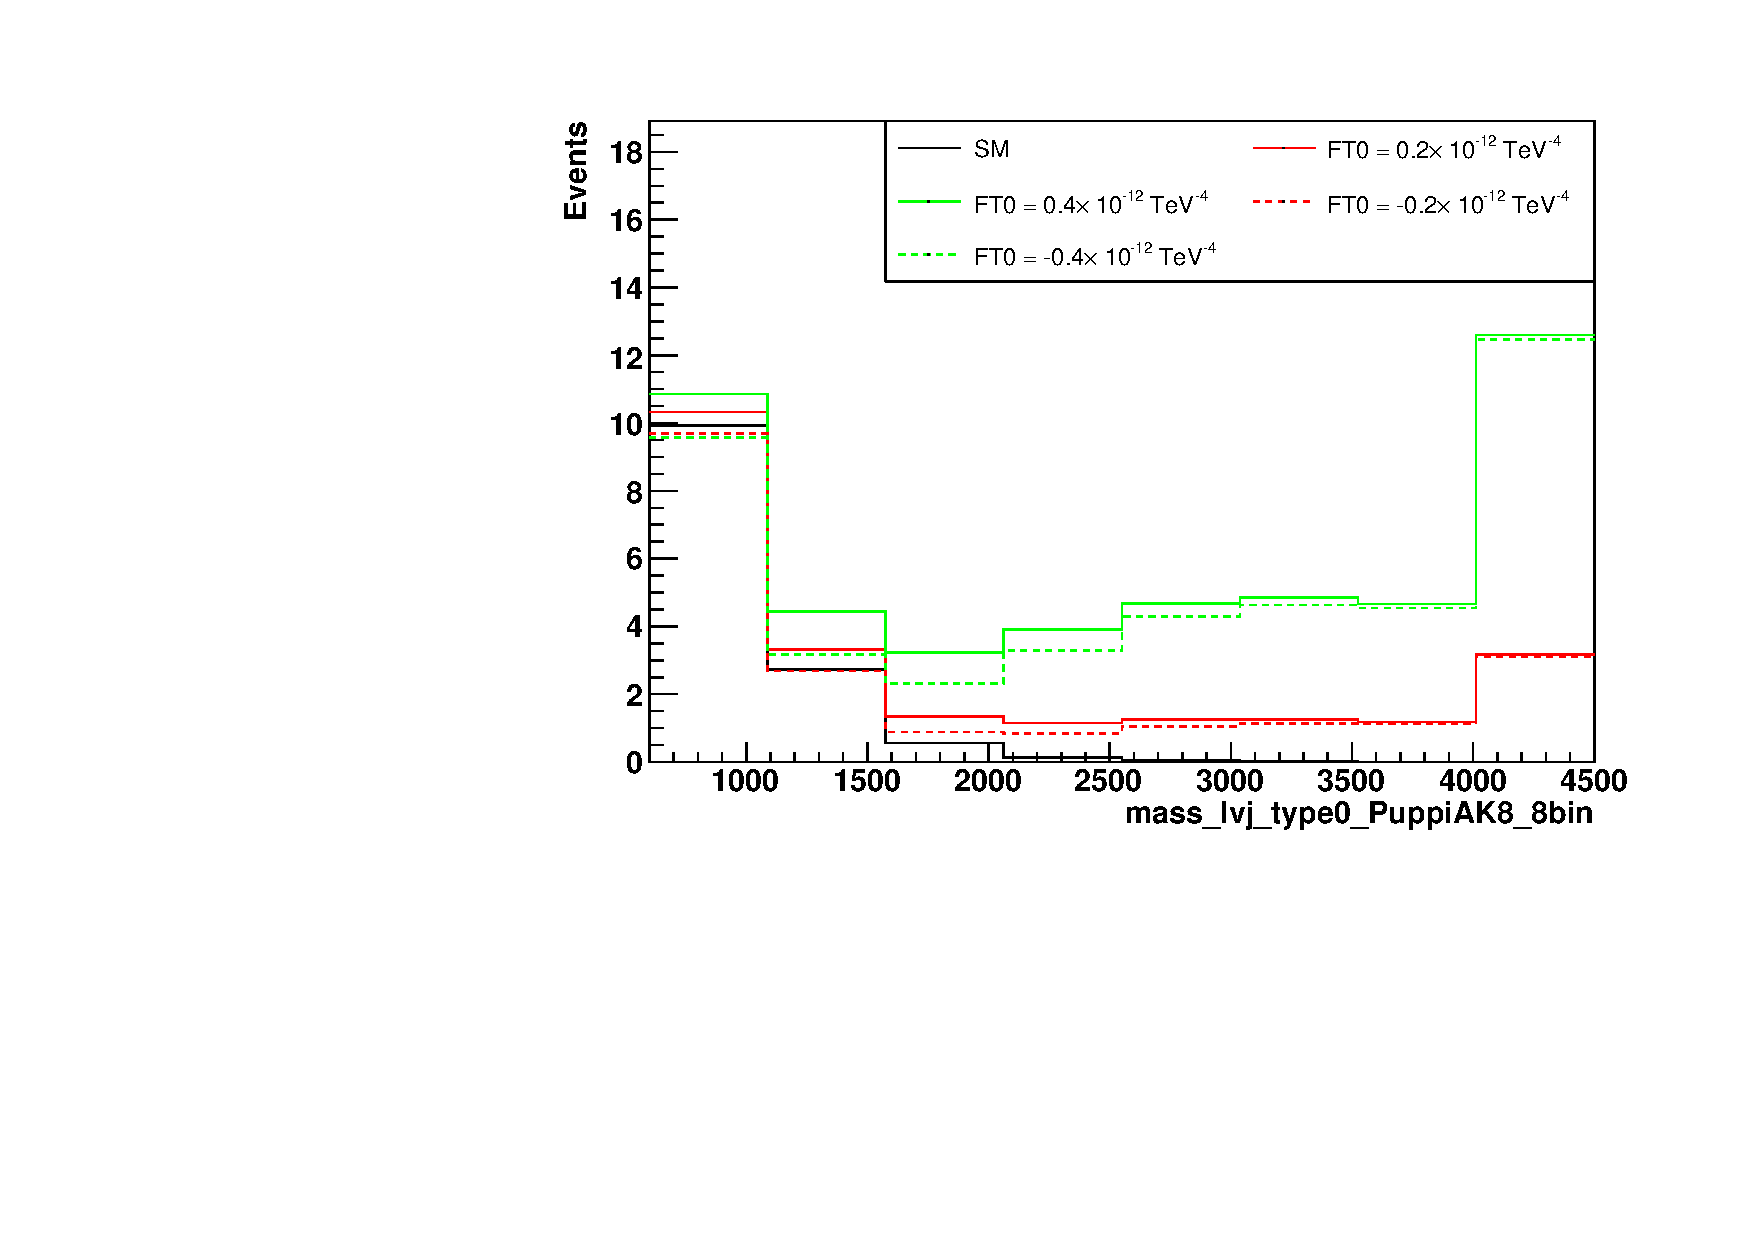
\includegraphics[width=0.40\textwidth]{Plots/aQGC_kinematics/mass_lvj_type0_PuppiAK8_8bin_FT0.pdf}\\
%   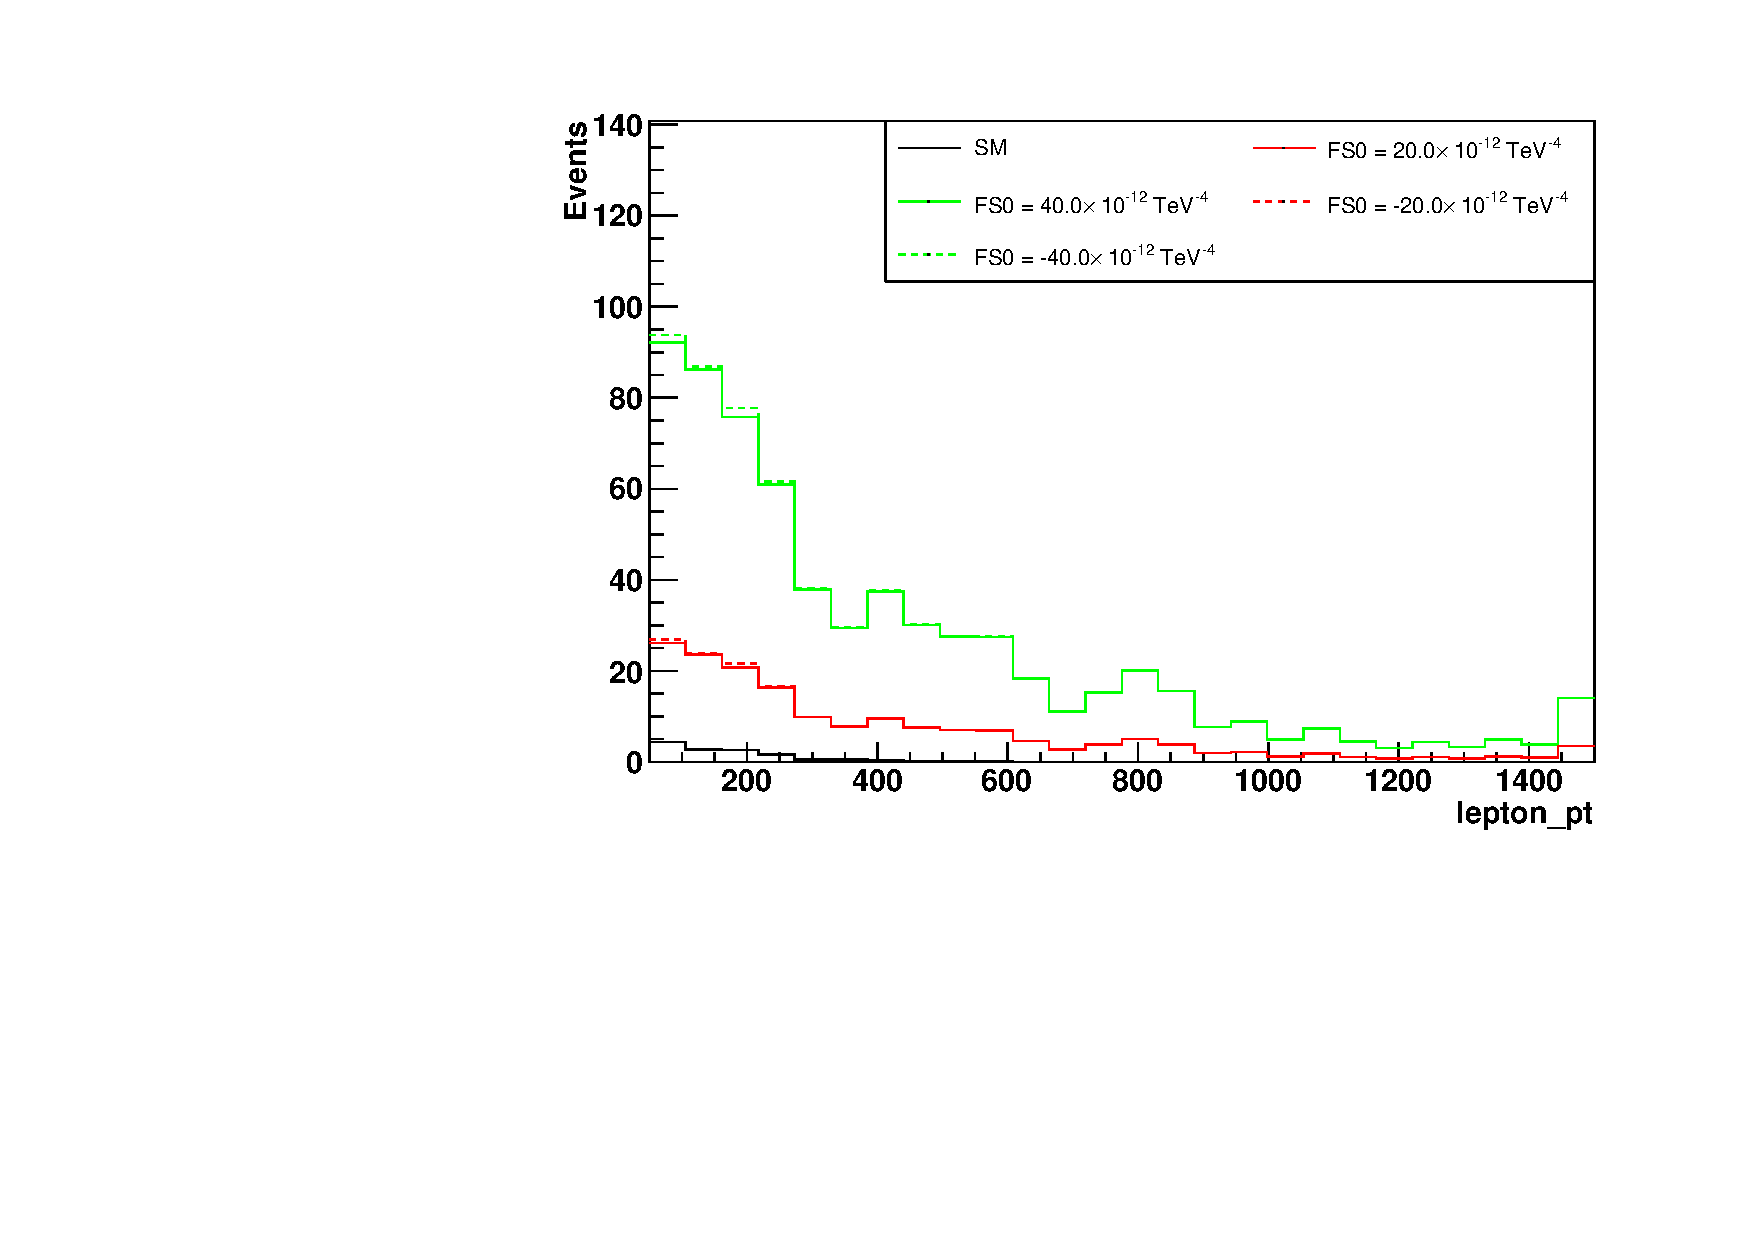
\includegraphics[width=0.40\textwidth]{Plots/aQGC_kinematics/lepton_pt_FS0.pdf}%
%   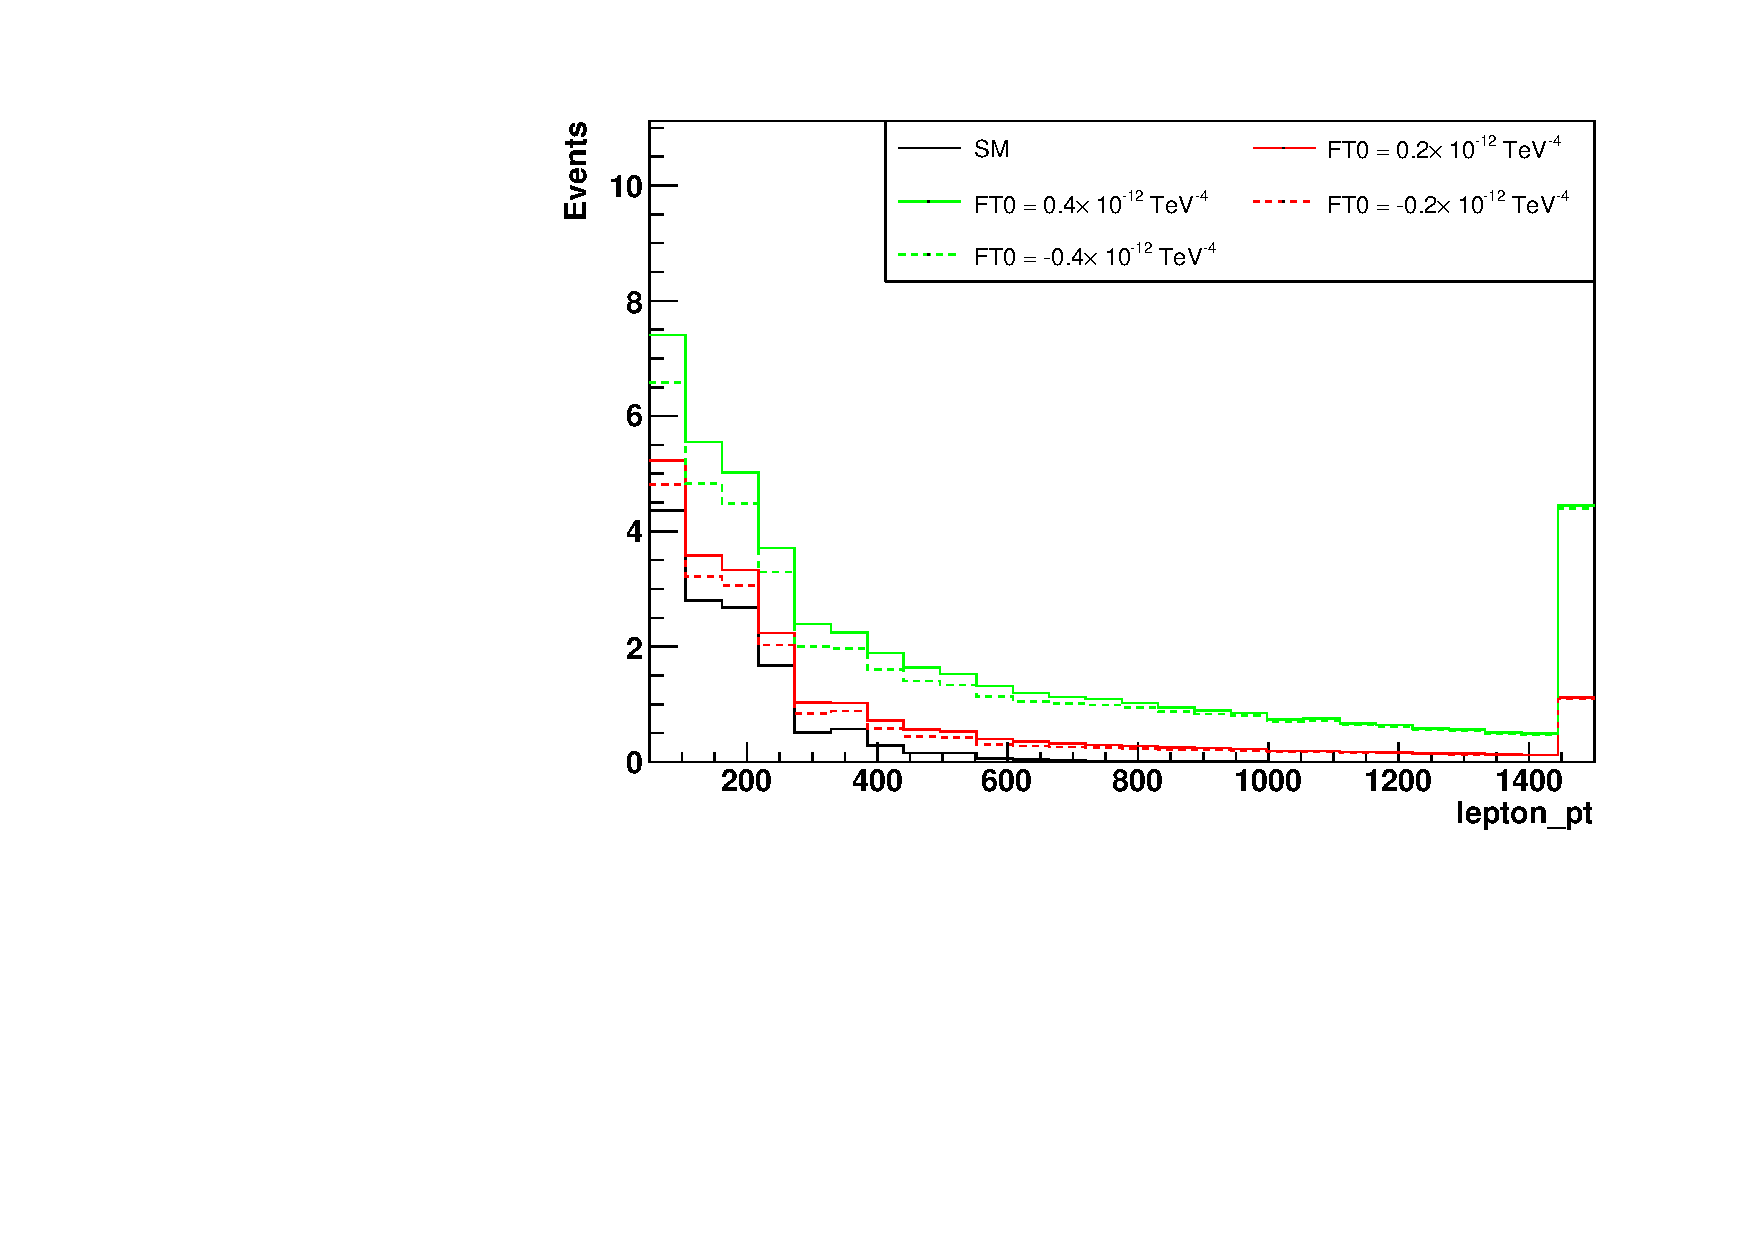
\includegraphics[width=0.40\textwidth]{Plots/aQGC_kinematics/lepton_pt_FT0.pdf}
%   \caption{Top: 4-body invariant mass showing for aQGC parameter FS0 (left) and FT0 (right). Bottom: lepton transverse momentum showing for aQGC parameter FS0 (left) and FT0 (right).}
%   \label{fig:mass_pt_sm_aqgc}
% \end{figure}


% \subsection{Comparison of MadSpin and Decay Package of MadGraph for Polarized Sample Generation}




%\subsection{Some useful links of forum}


\section{Sample Used} % (fold)
\label{sec:sample_used}
Several Monte Carlo (MC) event generators are used to simulate the signal and
background processes. For all processes, the detector response is simulated using a detailed description of the CMS detector, based on the \textsc{GEANT4} 
package~\cite{Agostinelli:2002hh}, and event reconstruction is performed with
the same algorithms as used for data. Proton-proton interactions occuring in the same beam crossing bin as the event of interest (pileup) are included in the simulation samples. The simulated events are weighted so that the pileup distribution matches the data, with an average pileup of about $27$ interactions per beam crossing.

\subsection{Data samples}

This analysis uses a sample of proton-proton collisions collected in 2016 with the CMS experiment at the LHC at $\sqrt{s} = 13~\rm{TeV}$.
Only data that passed the quality certification by all detector subsystems is used in the analysis using the golden JSON\footnote{In CMS, the information for the proton-proton collision runs which are considered as good and should be processed are kept in a file in JSON format (JSON stands for Java Script Object Notation.) using the information of luminosity sections. The JSON file that was used for 2016 run is
\\
\centerline{\small Cert\_271036-284044\_13TeV\_23Sep2016ReReco\_Collisions16\_JSON.txt}\\
This corresponding to an integrated luminosity of $35.9 \pm 0.9\fbinv$
} in order to select good data. {\it SingleMuon}  and {\it SingleElectron} primary datasets are used, which corresponds to the trigger that demands that there should be at least one muon and electrons, respectively in the collected data. The names of data samples used in the analysis are listed in Table~\ref{tab:datasample} 

\begin{table}[!htbp]
  \begin{center}
%{\tiny
  \begin{tabular}{l l}
\hline \textbf{Data stream} &  \textbf{Run and reconstruction version}  \\
\hline
SingleMuon      &       Run2016B-03Feb2017-v2       \\
SingleElectron  &       Run2016C-03Feb2017           \\
                &       Run2016D-03Feb2017           \\
		            &       Run2016E-03Feb2017          \\
                &       Run2016F-03Feb2017           \\
		            &       Run2016G-03Feb2017          \\
                &       Run2016H-03Feb2017-v1       \\
		            &       Run2016H-03Feb2017-v2       \\
                &       Run2016H-03Feb2017-v3       \\
\hline
  \end{tabular}
%}
  \caption{List of data samples used in the analysis. Here different run names corresponds to the different time stamp during which data was collected, and the date in the data sample name corresponds to the time stamp at wich it was converted to the physics objects, i.e, electrons, muons, jets, etc from the hit and energy deposit information.}
  \label{tab:datasample}
  \end{center}
\end{table}
 
 
\subsection{Simulated Samples}
The EW  processes with two final state quarks are simulated using \newline $\MADGRAPH{}5\_a\MCATNLO~2.3.3$~\cite{Alwall:2014} at leading-order (LO) with six electroweak (EWK) and zero quantum chromodynamics (QCD) vertices. The $\PW^{\pm}\PW^{\pm}$, $\PW^{\pm}\PW^{\mp}$,$\PW^{\pm}\PZ$, and $\PZ\PZ$ processes are produced separately. The complete list of the SM background samples can be found in Table~\ref{tab:signalSamples_sm} and Table~\ref{tab:signalSamples_aQGC}.
%
% \begin{table}[!htbp]
% \footnotesize
% \centering
% \begin{tabular}{lrr}
% \textbf{Sample name} & \textbf{Total events} & \textbf{Cross section[pb]} \\
% \hline
% /WplusToLNuWminusTo2JJJ\_{}EWK\_{}LO\_{}SM\_{}* & 1,991,279 & 0.9114\\
% /WplusTo2JWminusToLNuJJ\_{}EWK\_{}LO\_{}SM\_{}* & 1,994,040 & 0.9107\\
% /WplusToLNuWplusTo2JJJ\_{}EWK\_{}LO\_{}SM\_{}*  & 198,858   & 0.0879\\
% /WminusToLNuWminusTo2JJJ\_{}EWK\_{}LO\_{}SM\_{}*  & 199,535   & 0.0326\\
% /WplusToLNuZTo2JJJ\_{}EWK\_{}LO\_{}SM\_{}*    & 393,190   & 0.1825\\
% /WplusTo2JZTo2LJJ\_{}EWK\_{}LO\_{}SM\_{}*     & 198,932   & 0.0540\\
% /WminusToLNuZTo2JJJ\_{}EWK\_{}LO\_{}SM\_{}*   & 199,547   & 0.1000\\
% /WminusTo2JZTo2LJJ\_{}EWK\_{}LO\_{}SM\_{}*    & 198,910   & 0.0298\\
% /ZTo2LZTo2JJJ\_{}EWK\_{}LO\_{}SM\_{}*       & 100,000   & 0.0159\\
% \hline
% \hline
% /WplusToLNuWminusTo2JJJ\_{}EWK\_{}LO\_{}aQGC\_{}* & 1,981,940 & 17.940\\
% /WplusTo2JWminusToLNuJJ\_{}EWK\_{}LO\_{}aQGC\_{}* & 1,994,595 & 17.920\\
% /WplusToLNuWplusTo2JJJ\_{}EWK\_{}LO\_{}aQGC\_{}*  & 200,000   & 3.451\\
% /WminusToLNuWminusTo2JJJ\_{}EWK\_{}LO\_{}aQGC\_{}*& 200,000   & 0.507\\
% /WplusToLNuZTo2JJJ\_{}EWK\_{}LO\_{}aQGC\_{}*    & 399,232   & 1.895\\
% /WplusTo2JZTo2LJJ\_{}EWK\_{}LO\_{}aQGC\_{}*   & 199,238   & 0.569\\
% /WminusToLNuZTo2JJJ\_{}EWK\_{}LO\_{}aQGC\_{}*   & 200,000   & 0.741\\
% /WminusTo2JZTo2LJJ\_{}EWK\_{}LO\_{}aQGC\_{}*    & 198,620   & 0.222\\
% /ZTo2LZTo2JJJ\_{}EWK\_{}LO\_{}aQGC\_{}*     & 99,532    & 3.361\\
% \hline
% * = MJJ100PTJ10\_{}TuneCUETP8M1\_{}13TeV-madgraph-pythia8/ \\
%     RunIISummer16MiniAODv2-PUMoriond17\_{}80X\_{}mcRun2\_{}\\
%     asymptotic\_{}2016\_{}TrancheIV\_{}v6-v1/MINIAODSIM\\
% \hline
% \end{tabular}
% \caption{Signal sample names and cross sections of simulated samples used in the analysis}
% \label{tab:signalSamples}
% \end{table}
\begin{table}[!htbp]
\centering
{\scriptsize
\begin{tabular}{llrr}
\textbf{Process} &\textbf{Sample name} & \textbf{Total events} & \textbf{Cross section[pb]} \\
\hline
$pp \rightarrow W^+W^- JJ \rightarrow l^+ \nu JJ JJ$  & WplusToLNuWminusTo2JJJ\_{}EWK\_{}LO\_{}aQGC & 1,981,940 & 17.940\\
$pp \rightarrow W^+W^- JJ \rightarrow l^- \nu JJ JJ$  & WplusTo2JWminusToLNuJJ\_{}EWK\_{}LO\_{}aQGC & 1,994,595 & 17.920\\
$pp \rightarrow W^+W^+ JJ \rightarrow l^+ \nu JJ JJ$  & WplusToLNuWplusTo2JJJ\_{}EWK\_{}LO\_{}aQGC & 200,000   & 3.451\\
$pp \rightarrow W^-W^- JJ \rightarrow l^- \nu JJ JJ$  & WminusToLNuWminusTo2JJJ\_{}EWK\_{}LO\_{}aQGC & 200,000   & 0.507\\
$pp \rightarrow W^+Z JJ \rightarrow l^+ \nu JJ JJ$  & WplusToLNuZTo2JJJ\_{}EWK\_{}LO\_{}aQGC & 399,232   & 1.895\\
$pp \rightarrow W^+Z JJ \rightarrow l^+ l^- JJ JJ$  & WplusTo2JZTo2LJJ\_{}EWK\_{}LO\_{}aQGC  & 199,238   & 0.569\\
$pp \rightarrow W^-Z JJ \rightarrow l^- \nu JJ JJ$  & WminusToLNuZTo2JJJ\_{}EWK\_{}LO\_{}aQGC & 200,000   & 0.741\\
$pp \rightarrow W^-Z JJ \rightarrow l^+ l^- JJ JJ$  & WminusTo2JZTo2LJJ\_{}EWK\_{}LO\_{}aQGC & 198,620   & 0.222\\
$pp \rightarrow ZZ JJ \rightarrow l^+ l^- JJ JJ$  & ZTo2LZTo2JJJ\_{}EWK\_{}LO\_{}aQGC & 99,532    & 3.361\\
\hline
\end{tabular}
\caption{aQGC signal sample names and cross sections of simulated samples used in the analysis}
\label{tab:signalSamples_aQGC}
}
\end{table}
%
\begin{table}[!htbp]
\centering
{\scriptsize
\begin{tabular}{llrr}
\textbf{Process} &\textbf{Sample name} & \textbf{Total events} & \textbf{Cross section[pb]} \\
\hline
$pp \rightarrow W^+W^- JJ \rightarrow l^+ \nu JJ JJ$  & WplusToLNuWminusTo2JJJ\_{}EWK\_{}LO\_{}aQGC & 1,991,279 & 0.9114\\
$pp \rightarrow W^+W^- JJ \rightarrow l^- \nu JJ JJ$  & WplusTo2JWminusToLNuJJ\_{}EWK\_{}LO\_{}aQGC & 1,994,040 & 0.9107\\
$pp \rightarrow W^+W^+ JJ \rightarrow l^+ \nu JJ JJ$  & WplusToLNuWplusTo2JJJ\_{}EWK\_{}LO\_{}aQGC & 198,858   & 0.0879\\
$pp \rightarrow W^-W^- JJ \rightarrow l^- \nu JJ JJ$  & WminusToLNuWminusTo2JJJ\_{}EWK\_{}LO\_{}aQGC & 199,535   & 0.0326\\
$pp \rightarrow W^+Z JJ \rightarrow l^+ \nu JJ JJ$  & WplusToLNuZTo2JJJ\_{}EWK\_{}LO\_{}aQGC & 393,190   & 0.1825\\
$pp \rightarrow W^+Z JJ \rightarrow l^+ l^- JJ JJ$  & WplusTo2JZTo2LJJ\_{}EWK\_{}LO\_{}aQGC  & 198,932   & 0.0540\\
$pp \rightarrow W^-Z JJ \rightarrow l^- \nu JJ JJ$  & WminusToLNuZTo2JJJ\_{}EWK\_{}LO\_{}aQGC & 199,547   & 0.1000\\
$pp \rightarrow W^-Z JJ \rightarrow l^+ l^- JJ JJ$  & WminusTo2JZTo2LJJ\_{}EWK\_{}LO\_{}aQGC & 198,910   & 0.0298\\
$pp \rightarrow ZZ JJ \rightarrow l^+ l^- JJ JJ$  & ZTo2LZTo2JJJ\_{}EWK\_{}LO\_{}aQGC & 100,000   & 0.0159\\
\hline
\end{tabular}
\caption{SM EWK signal sample names and cross sections of simulated samples used in the analysis}
\label{tab:signalSamples_sm}
}
\end{table}
%
%
The QCD initiated production of two gauge bosons with two final state quarks (which we refer to as diboson process) and at least one QCD vertex is considered as background. \MADGRAPH{}5\_a\MCATNLO at LO is used to simulate this sample. The interference between the EWK and QCD diagrams is evaluated using dedicated samples produced with the \textsc{Phantom}~1.2.8~\cite{Ballestrero:2007xq}\todo[inline]{Add details of Phantom generator.} generator and is found to be negligible compared to the theoretical uncertainties. Figure~\ref{fig:interference} shows the level of the interference contribution. 

\begin{figure*}[!htbp]
\centering
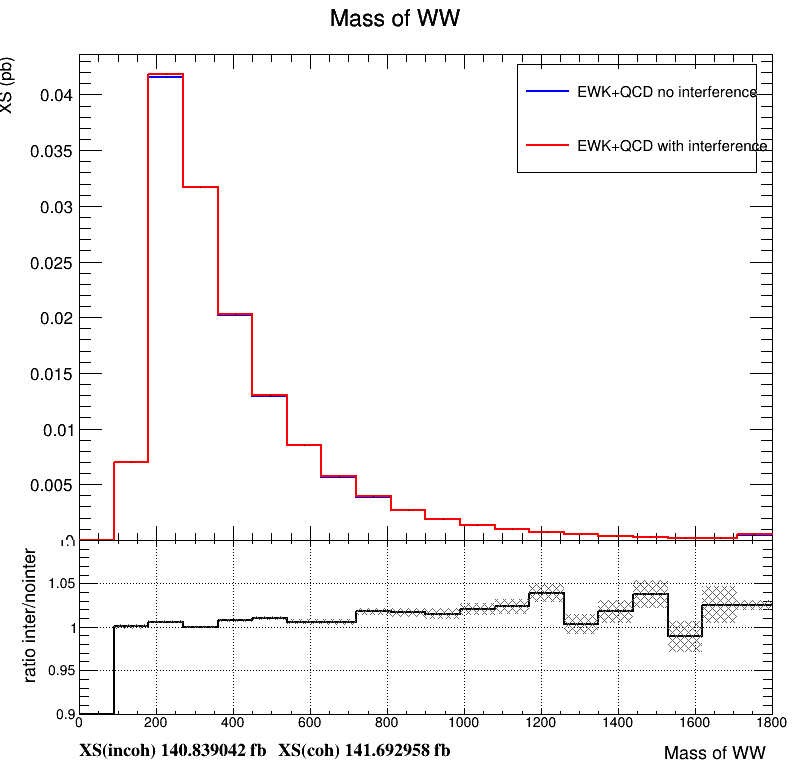
\includegraphics[width=0.45\textwidth]{Plots/plots/interference_comparison_mww.png}
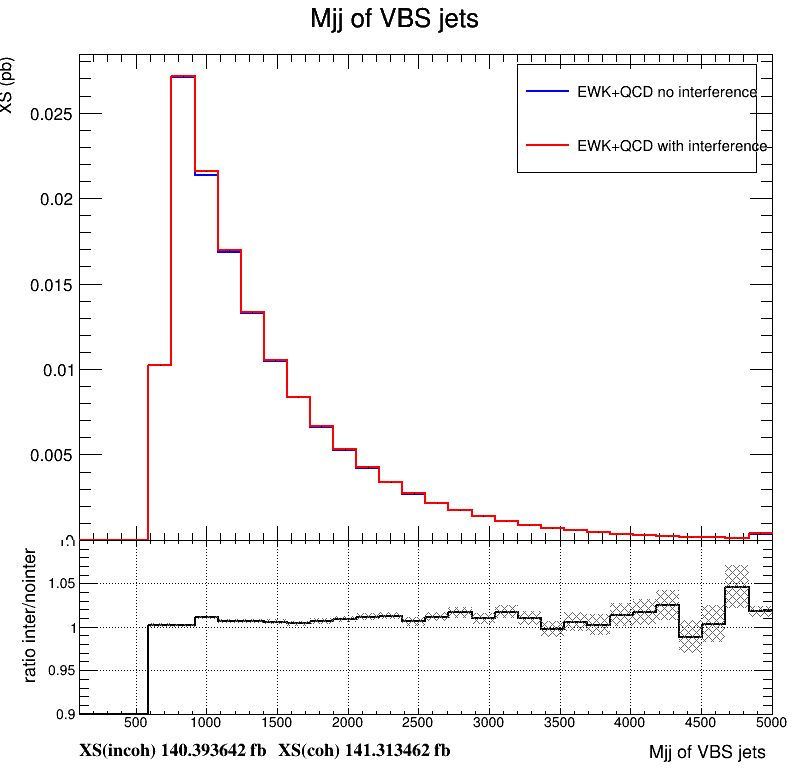
\includegraphics[width=0.45\textwidth]{Plots/plots/interference_comparison_mjj_vbs.png}
\caption{Distributions of $m_{\PW V}$ (left) and $m_{jj}$ (right) in the signal region with interference contribution (red) and without intereference contribution (blue).}
\label{fig:interference}
\end{figure*}

The aQGC signal samples are produced using \MADGRAPH{}5\_a\MCATNLO at LO accuracy. The default coupling for the event generation is set to $f_{T0} / \Lambda^{4} = -12.5 [\mathrm{TeV}]^{-4}$. Other coupling strengths are obtained by means of the reweighting method in \MADGRAPH{}5\_a\MCATNLO~\cite{Mattelaer2016,Mattelaer-reweight}. Figure~\ref{fig:aqgc_signal} shows the mass distributions of the  $\PW \PW$ system for few aQGC parameters for the operators $S0$ (left) and $T2$ (right). The expected enhancement of the production cross section at large masses for nonzero aQGC is clearly seen.      
  
\begin{figure*}[!htbp]
\centering
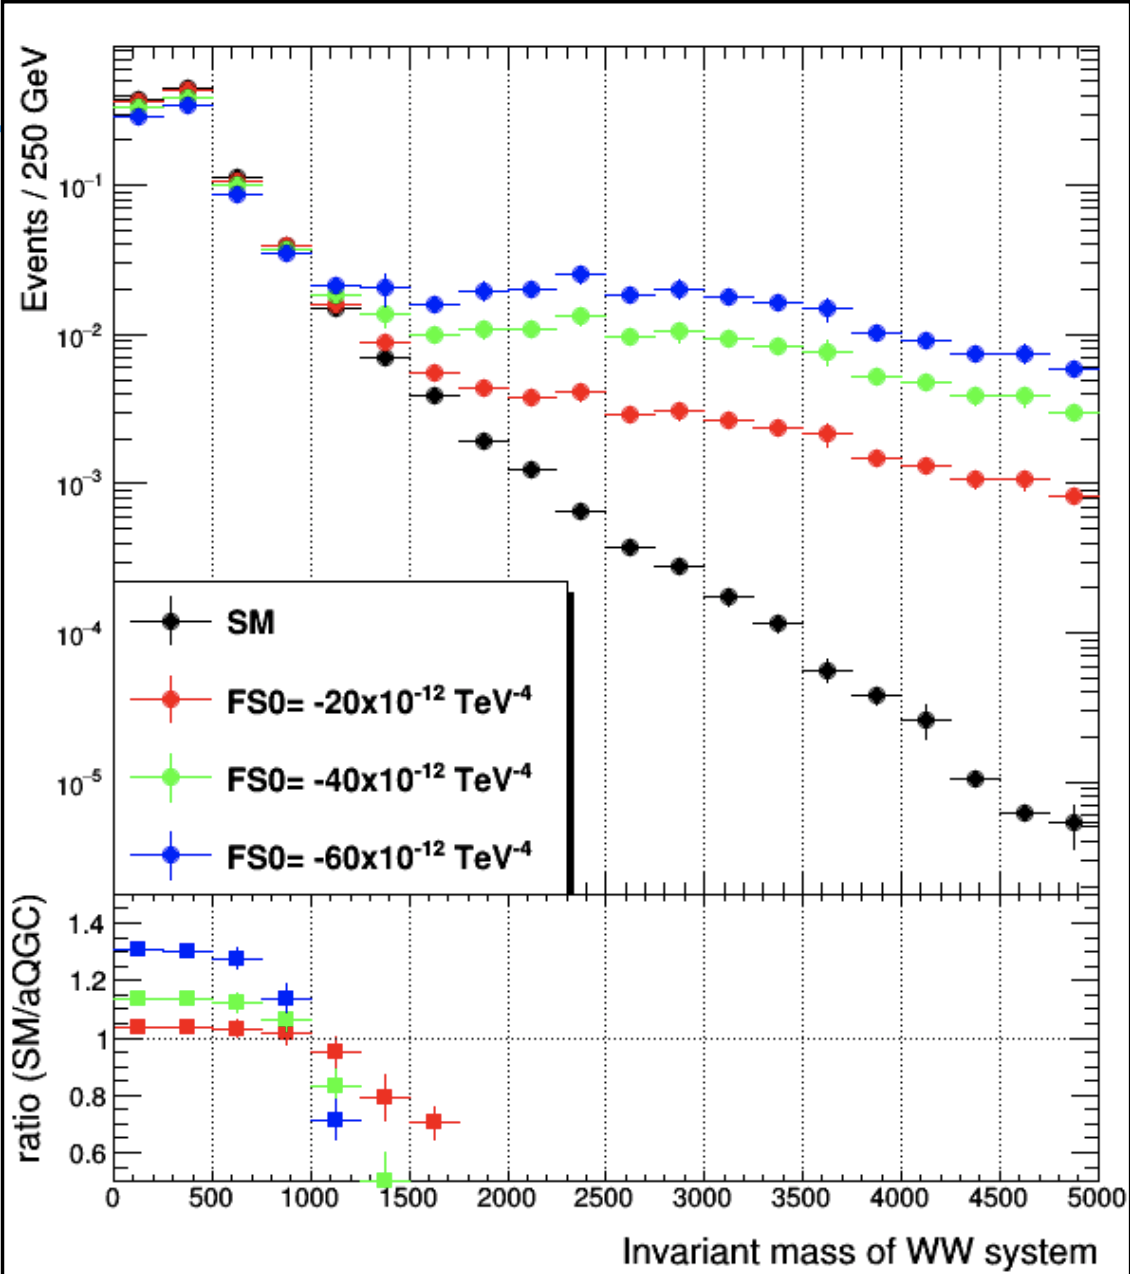
\includegraphics[width=0.45\textwidth]{Plots/aQGC_Signal_Scaling/mWW_FS0.png}
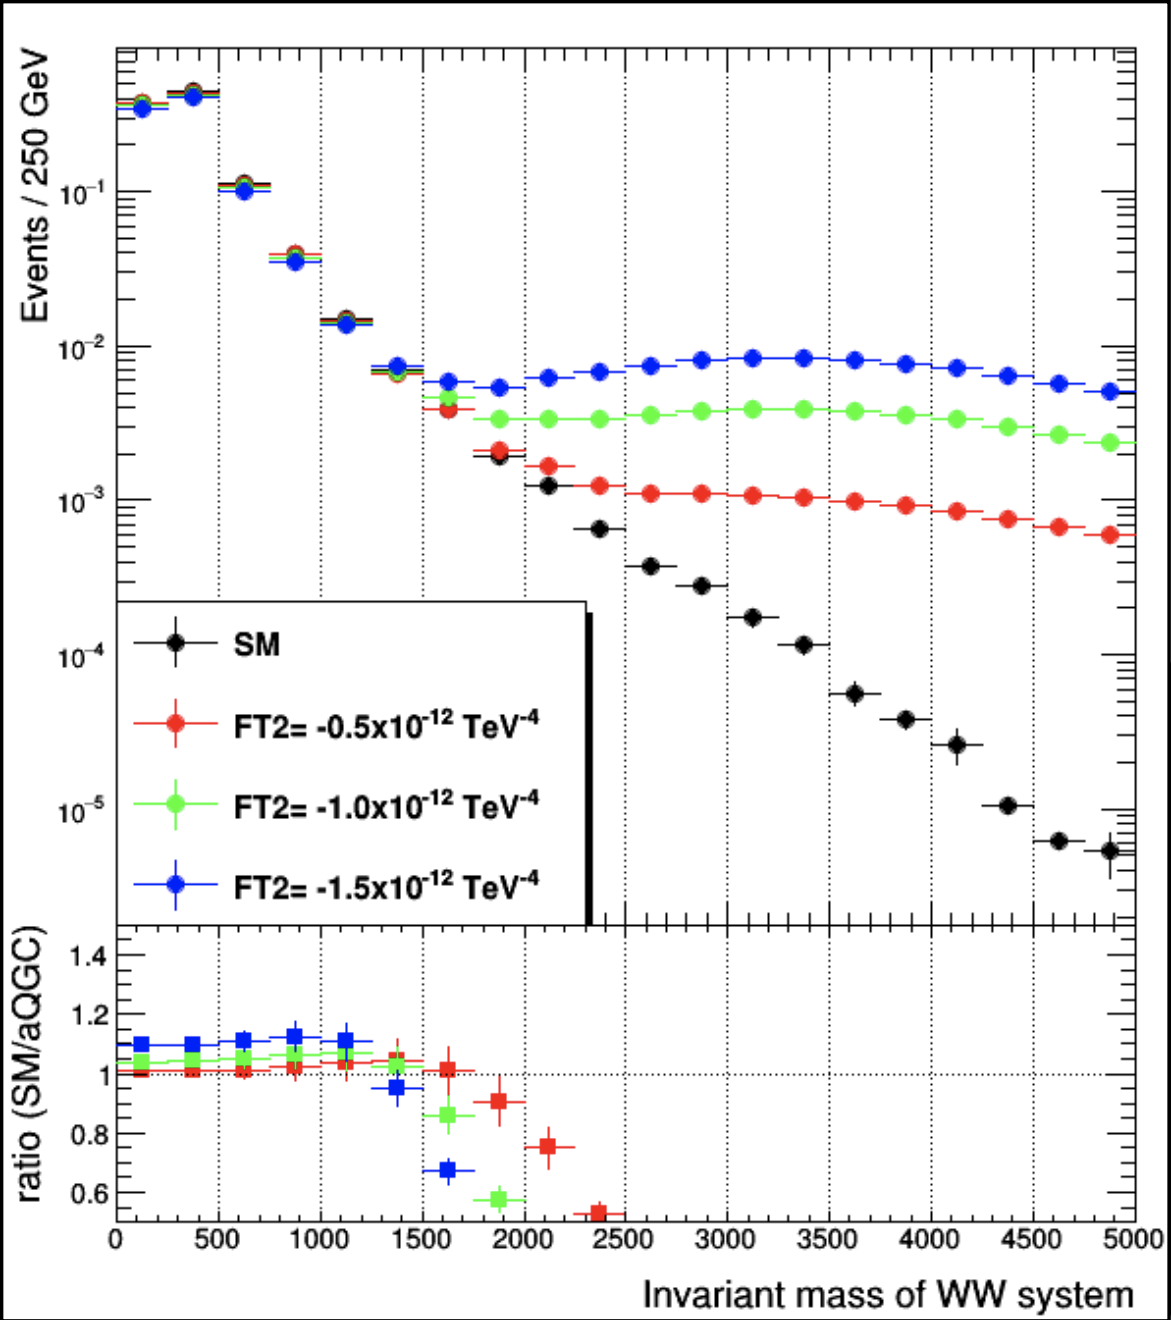
\includegraphics[width=0.45\textwidth]{Plots/aQGC_Signal_Scaling/mWW_FT2.png}
\caption{Mass distributions of the $\PW \PW$ system for the SM EW and few aQGC parameters for the operators $S0$ (left) and $T2$ (right).}
\label{fig:aqgc_signal}
\end{figure*}



The Drell--Yan process is simulated with one, two, three, and four outgoing partons at Born level at LO using \MADGRAPH{}5\_a\MCATNLO. The $\PW+$jets process is simulated at LO using \MADGRAPH{}5\_a\MCATNLO. $\ttbar$, $\ttbar \PW$, $\ttbar \PZ$, and single top processes are generated at next-to-leading order (NLO) using \textsc{POWHEG2.0}~\cite{Alioli:2008gx,Nason:2004rx,Frixione:2007vw,powheg:2010}. The simulated samples of background processes are normalized to the best theoretical prediction. The complete list of background samples can be found in Table~\ref{tab:bkgSamples}.

The \PYTHIA~8.205~\cite{Sjostrand:2015} package is used  for parton showering, hadronization, and the underlying event simulation, with tune CUETP8M1~\cite{Skands:2014pea,Khachatryan:2015pea}. The NNPDF~3.0~\cite{nnpdf} set is used as the default set of parton distribution functions (PDFs). The PDFs are calculated to the same order in QCD as the hard process. 
% %
% \begin{table}[!htbp]
% \footnotesize
% \centering
% % \topcaption{Sample names and cross sections of simulated samples used in the analysis.}
%  {\scriptsize
% % \begin{tabular}{p{9cm}r}
% \begin{tabular}{lr}
% \textbf{Sample name} & \textbf{Cross section[pb]} \\
% \hline
% WJetsToLNu\_{}HT-100To200\_{}TuneCUETP8M1\_{}13TeV-madgraphMLM-pythia8  & 1345*1.21 \\
% WJetsToLNu\_{}HT-200To400\_{}TuneCUETP8M1\_{}13TeV-madgraphMLM-pythia8 & 359.7*1.21 \\
% WJetsToLNu\_{}HT-400To600\_{}TuneCUETP8M1\_{}13TeV-madgraphMLM-pythia8 & 48.91*1.21 \\
% WJetsToLNu\_{}HT-600To800\_{}TuneCUETP8M1\_{}13TeV-madgraphMLM-pythia8 & 12.05*1.21 \\
% WJetsToLNu\_{}HT-800To1200\_{}TuneCUETP8M1\_{}13TeV-madgraphMLM-pythia8 & 5.501*1.21 \\
% WJetsToLNu\_{}HT-1200To2500\_{}TuneCUETP8M1\_{}13TeV-madgraphMLM-pythia8 & 1.329*1.21 \\
% WJetsToLNu\_{}HT-2500ToInf\_{}TuneCUETP8M1\_{}13TeV-madgraphMLM-pythia8 & 0.03216*1.21 \\
% \hline
% WplusToLNuWminusTo2JJJ\_{}EWK\_{}LO\_{}QCD\_{}*	&	5.544\\
% WplusTo2JWminusToLNuJJ\_{}EWK\_{}LO\_{}QCD\_{}*	&	5.561\\
% WplusToLNuWplusTo2JJJ\_{}EWK\_{}LO\_{}QCD\_{}*	        &	0.08642\\
% WminusToLNuWminusTo2JJJ\_{}EWK\_{}LO\_{}QCD\_{}*       &	0.03774\\
% WplusToLNuZTo2JJJ\_{}EWK\_{}LO\_{}QCD\_{}*		&	2.162\\
% WplusTo2JZTo2LJJ\_{}EWK\_{}LO\_{}QCD\_{}*		&	0.6409\\
% WminusToLNuZTo2JJJ\_{}EWK\_{}LO\_{}QCD\_{}*		&	1.302\\
% WminusTo2JZTo2LJJ\_{}EWK\_{}LO\_{}QCD\_{}*		&	0.3862\\
% ZTo2LZTo2JJJ\_{}EWK\_{}LO\_{}QCD\_{}*			&	0.3756\\
% \hline
% TT\_{}TuneCUETP8M1\_{}13TeV-powheg-pythia8 & 831.76 \\
% \hline
% ST\_{}s-channel\_{}4f\_{}leptonDecays\_{}13TeV-amcatnlo-pythia8\_{}TuneCUETP8M1 & 3.68 \\
% ST\_{}t-channel\_{}top\_{}4f\_{}inclusiveDecays\_{}13TeV-powhegV2-madspin-pythia8\_{}TuneCUETP8M1 & 136.02 \\
% ST\_{}t-channel\_{}antitop\_{}4f\_{}inclusiveDecays\_{}13TeV-powhegV2-madspin-pythia8\_{}TuneCUETP8M1 & 80.95 \\
% ST\_{}tW\_{}antitop\_{}5f\_{}inclusiveDecays\_{}13TeV-powheg-pythia8\_{}TuneCUETP8M1 & 35.6 \\
% ST\_{}tW\_{}top\_{}5f\_{}inclusiveDecays\_{}13TeV-powheg-pythia8\_{}TuneCUETP8M1 & 35.6 \\
% \hline
% DY1JetsToLL\_M-50\_TuneCUETP8M1\_13TeV-madgraphMLM-pythia8 & 1012 \\
% DY2JetsToLL\_M-50\_TuneCUETP8M1\_13TeV-madgraphMLM-pythia8 & 335 \\
% DY3JetsToLL\_M-50\_TuneCUETP8M1\_13TeV-madgraphMLM-pythia8 & 102 \\
% DY4JetsToLL\_M-50\_TuneCUETP8M1\_13TeV-madgraphMLM-pythia8 & 54 \\
% %QCD\_HT200to300\_TuneCUETP8M1\_13TeV-madgraphMLM-pythia8 & 1717000 \\
% %QCD\_HT300to500\_TuneCUETP8M1\_13TeV-madgraphMLM-pythia8 & 351300 \\
% %QCD\_HT500to700\_TuneCUETP8M1\_13TeV-madgraphMLM-pythia8 & 31630 \\
% %QCD\_HT700to1000\_TuneCUETP8M1\_13TeV-madgraphMLM-pythia8 & 6802 \\
% %QCD\_HT1000to1500\_TuneCUETP8M1\_13TeV-madgraphMLM-pythia8 & 1206 \\
% %QCD\_HT1500to2000\_TuneCUETP8M1\_13TeV-madgraphMLM-pythia8 & 120.4 \\
% %QCD\_HT2000toInf\_TuneCUETP8M1\_13TeV-madgraphMLM-pythia8 & 25.25 \\
% %\hline
% \end{tabular}
% }
% \caption{Background sample names and cross sections of simulated samples used in the analysis. The naming }
% \label{tab:bkgSamples}
% \end{table}

%
\begin{table}[!htbp]
\footnotesize
\centering
% \topcaption{Sample names and cross sections of simulated samples used in the analysis.}
 {\scriptsize
% \begin{tabular}{p{9cm}r}
\begin{tabular}{lr}
\textbf{Sample name} & \textbf{Cross section[pb]} \\
\hline
WJetsToLNu HT bins 100 to 200 GeV & 1345*1.21 \\
WJetsToLNu HT bins 200 to 400 GeV  & 359.7*1.21 \\
WJetsToLNu HT bins 400 to 600 GeV & 48.91*1.21 \\
WJetsToLNu HT bins 600 to 800 GeV & 12.05*1.21 \\
WJetsToLNu HT bins 800 to 1200 GeV & 5.501*1.21 \\
WJetsToLNu HT bins 1200 to 2500 GeV & 1.329*1.21 \\
WJetsToLNu HT bins 2500 GeV to Inf  & 0.03216*1.21 \\
\hline
TTbar & 831.76 \\
\hline
Single Top production s-channel & 3.68 \\
Single Top production t-channel & 136.02 \\
Single Anti-Top production t-channel & 80.95 \\
Single Anti-Top production tW-channel & 35.6 \\
Single Top production tW-channel & 35.6 \\
\hline
Drell-Yan + 1 jet  & 1012 \\
 Drell-Yan + 2 jet & 335 \\
 Drell-Yan + 3 jet & 102 \\
 Drell-Yan + 4 jet & 54 \\
 \hline
\end{tabular}
}
\caption{Background sample names and cross sections of simulated samples used in the analysis. The naming }
\label{tab:bkgSamples}
\end{table}



% section sample_used (end)

\section{Object Selection} % (fold)
\label{sec:object_selection}
A set of standard objects used in this analysis is summarized in Table~\ref{tab:objects_final}. More details are given below.  

\begin{table}[!htbp]
  \begin{center}
 {\small
  \begin{tabular} {lc}
\hline
  Objects      & Selections \\
  \hline
Triggers       & Single lepton triggers  \\
Primary vertex & Nominal selection  \\
jets           & PF jets, anti-$k_{\rm T}$, $\Delta R = 0.4$  \\
$V$ jets       & Puppi+SD, anti-$k_{\rm T}$, $\Delta R = 0.8$ \\
$\met$         & Type-1 PF $\met$\\
B-tagging      & CSVv2 {\em``Loose''}  \\
Electrons      & tight POG identification criteria  \\
Muons          & tight POG identification criteria   \\
  \hline
  \end{tabular}
}
  \caption{Summary of object selection.}
  \label{tab:objects_final}
  \end{center}
\end{table}

%%%%%%%%%%%
%%%%%%%%%%%
\subsection{Trigger}
\label{subsec:trigger}
The data samples used in the analysis were taken with the following triggers:
\begin{itemize}
\item HLT\_Ele27\_WPTight\_Gsf\_v* (electron channel)
\item HLT\_IsoTkMu24\_v* or  HLT\_IsoMu24\_v* (muon channel)
\end{itemize}
The explanation of these triggers are given in Table~\ref{tab:trigger-path}. The trigger efficiencies in data and simulation are measured using tag-and-probe~\cite{Tag_probe}. In tag-and-probe method the correction factors  for the values extracted from the simulation are determined using $Z \rightarrow l^+ l^-$ sample in both data and simulation. This removes any systematic uncertainty coming from imperfections in the simulation. For the measurement for a given efficiency contains events selected with two lepton candidates. The first lepton, known as ``\textit{tag}'', was choosen based on the tight identification and isolation requirements. The other leptons, known as ``\textit{probe}'', is selected based on the criteria which depends on the efficiency being measured. The invariant mass of the choosen tag and probe lepton candidate should fall in the range of 60-120 \GeV. The signal yields are obtained for two exclusive subsamples of events in which the probe lepton passes or fails the selection criteria considered. Fits are performed to the invariant-mass distribution of the pass and fail subsamples, including a term that accounts for the background. The measured efficiency is deduced from the relative level of signal in the pass and fail subsamples; its uncertainty includes a systematic contribution from the fitting procedure. The correction factors are obtained as ratios of tag-and-probe efficiencies for the data and for the simulation. The ratio of data and simulation efficiencies is found to be consistent with unity within 1\%.


%%%%%%%%%%%
%%%%%%%%%%%
\subsection{Electron selection}
\label{subsec:electrons}
Electron selection variables are categorized into three groups: identification (ID) variables, isolation variables and conversion rejection variables~\cite{ElectronReconstruction_8TeV_cms,Novakova2013}.

The most powerful ID variables for the electron identification are:
\begin{enumerate}
  \item the energy-momentum match between the seed cluster and the track, $E_{seed}/p_{in}$,
  \item the variables measuring spatial matching between the track and the supercluster, $\Delta \eta_{in}$ and $\Delta \phi_{in}$,
  \item the supercluster $\eta$ width, $\sigma_{i\eta i\eta}$, taken from the covariance matrix using the logarithmic weights, and
  \item the hadronic leakage variable $H/E$.
\end{enumerate}

The isolation of the electron candidates is computed from the flux of PF candidates found within a cone of $\Delta R = 0.4$ built around the lepton direction.
The flux of particles is computed independently for the charged hadrons, neutral hadrons and photon candidates. When dealing with electron candidates, the neutral flux is corrected by using the average energy density due to
pileup and underlying event in the central region of the detector ($\rho$)
and an effective area ($A_{\rm eff}$) correction which normalizes this
estimator in such a way that the isolation is independent of the number of pileup interactions. The electron isolation is therefore defined as:

\begin{equation}
I^{e}_{\rm rel}=\frac{1}{p_{\rm T}}  \left[ I_{\rm ch}+\max(I_{\rm nh}+I_{\rm g}-A_{\rm eff}\cdot\rho,0) \right]
\label{eq:eleisol}
\end{equation}

Now for the conversion rejection three sets of variables are used. The transverse impact parameter is used to discriminate electrons from conversion as they will have, on average, a greater distance to the beam position. We also expect an electron from a conversion to have missing hits in the innermost tracker layer.

Finally based on the above explanation the electrons identification variables are divided into the three categories based on the cuts with increasing background rejection power and decreasing signal efficiency: tight, medium, loose, veto and also in the endcap and barrel. All these parameters are summarized in Table~\ref{table:electron-identification} and Table~\ref{table:electron-identification-2}.

\begin{table}
\centering
\begin{tabular}[!htbp]{l c c c c}
\hline
{\textbf{Variables}} & {\textbf{Veto}} & \textbf{Loose} & \textbf{Medium} &  \textbf{Tight} \\
\hline
$\sigma_{i\eta i\eta} < $ & 0.0115  & 0.011   & 0.00998 & 0.00998 \\
$|\Delta \eta_{in}| < $   & 0.00749 & 0.00477 & 0.00311 & 0.00308 \\
$\Delta \phi_{in} < $     & 0.228   & 0.222   & 0.103   & 0.0816  \\
$H/E < $                  & 0.356   & 0.298   & 0.253   & 0.0414  \\
$I^{e}_{\rm rel} < $      & 0.175   & 0.0994  & 0.0695  & 0.0588  \\
$|1/E - 1/p| < $          & 0.299   & 0.241   & 0.134   & 0.0129  \\
expected missing inner hits $<=$ & 2  & 1   &   1   &   1 \\
pass conversion veto      & yes   & yes & yes & yes \\
\hline
\end{tabular}
\caption{The cut based electron identification working points for $|\eta \text{ supercluster}| <= 1.479$ .}
\label{table:electron-identification}
\end{table}
\begin{table}
\centering
\begin{tabular}[!htbp]{l c c c c}
\hline
{\textbf{Variables}} & {\textbf{Veto}} & \textbf{Loose} & \textbf{Medium} &  \textbf{Tight} \\
\hline
$\sigma_{i\eta i\eta} < $ & 0.037   & 0.0314 & 0.0298 & 0.0292    \\
$|\Delta \eta_{in}| < $   & 0.00895 & 0.00868& 0.00609& 0.00609   \\
$\Delta \phi_{in} < $     & 0.213   & 0.213  & 0.045  & 0.0394    \\
$H/E < $                  & 0.211   & 0.101  & 0.0878 & 0.0641    \\
$I^{e}_{\rm rel} < $      & 0.159   & 0.107  & 0.0821 & 0.0571   \\
$|1/E - 1/p| < $          & 0.15    & 0.14   & 0.13   & 0.0129    \\
expected missing inner hits $<=$ & 3& 1   &   1   &   1 \\
pass conversion veto      & yes     & yes & yes & yes \\
\hline
\end{tabular}
\caption{The cut based electron identification working points for $|\eta \text{ supercluster}| > 1.479$ .}
\label{table:electron-identification-2}
\end{table}

For this analysis the electrons are selected using the {\em ``Tight''} ID. In addition, an electron veto is applied with the {\em ``Loose''} ID, to reject events with more than two genuine leptons. 

Furthermore, the scale factors are used to correct for differences in the reconstruction, identification and isolation efficiencies between data and simulation. They are evaluated using the tag and probe technique, considering the scale factors and their uncertainty both.
 

%%%%%%%%%%%%%%%
%%%%%%%%%%%%%%%
\subsection{Muon selection}
For muons reconstruction two approaches are used:
\begin{enumerate}
  \item \textbf{the global muon reconstruction (outside-in)}: In this case, a tracker-track is found for each standalone-muon track and a combined fit of the tracker and muon-detector hits is performed, using the Kalman-filter technique~\cite{Kalman1960,Fruehwirth1987}.
  \item \textbf{the tracker muon reconstruction (inside-out)}: Here, the tracker-track is extrapolated and matched to segments reconstructed in the muon detector and it is said to be matched if the distance between them is less than 3 cm or if the value of the pull is less than 4, where the pull is defined as the difference between the position of the matched segment and the position of the extrapolated track, divided by their combined uncertainties.
\end{enumerate}

At low momenta, $p \leq 5 ~GeV$, the tracker muon reconstruction is more efficient than the global muon reconstruction, as it requires only a single muon segment in the muon system, whereas the global muon reconstruction is designed to have high efficiency for muons penetrating through more than one muon station and typically requires segments in at least two muon stations.

For muon identification there are six different algorithms are commonly used in CMS. They are Loose Muons, Medium Muons, Tight Muons, Soft Muons, High $p_T$ Muons, and High $p_T$ Tracker Muons. Here only Loose and Tight muon selections are described which are used in the analysis~\cite{Kraetschmer2016}.
\begin{enumerate}
  \item \textbf{Loose muon selection:} This requires a candidate to be reconstructed by the particle-flow algorithm~\cite{Particle_flow_2010} and a global or a tracker-muon.
  % \item \textbf{Soft muon selection:} This requires a tracker-muon having tight requirements on the matched muon segment, on the number of hits, the track $\chi^2$, and the impact parameters;
  \item \textbf{Tight muon selection:} This requires the particle to be identified as muons by the particle flow event reconstruction and as global as well as the tracker muon with requirements on the hits, global track $\chi^2$, and the impact parameters.
\end{enumerate}

The muons are selected using the {\em``Tight''} muon identification mentioned above.
Additionally, like in the electron case, a third muon veto is also applied to reject events with more than two genuine leptons using the {\em``Loose''} identification. 
For the muon isolation, in the same manner as for electrons, a cone of $\Delta R = 0.4$ is built to compute the flux of particle flow candidates, the ``delta-beta'' correction\footnote{The vertex association of leptons does not account for the neutral particles produced by the pile-up interactions. To consider the missed neutral particles, a specific correction is applied, which is known as ``delta-beta'' corrections. It uses the particle based isolation to preedict the neutral particle deposits in the isolation cone based on particle deposits due to pile-up in the same cone.} is applied to correct for pileup contamination~\cite{Bachtis2013}.
This correction is achieved by subtracting half the sum of the \pt of the charged particles in the cone of interest but with particles not originating from the primary vertex.

The muon isolation is therefore defined as:
\begin{equation}
I^{\mu}_{\rm rel}=\frac{1}{p_{\rm T}}  \left[ I_{\rm ch}+\max(I_{\rm nh}+I_{\rm g}-0.5\cdot I_{\rm chPU} ,0) \right]
\label{eq:muisol}
\end{equation}
 
Scale factors are used to correct for differences in the reconstruction, identification and isolation efficiencies between data and simulation. They are evaluated using the tag and probe technique, using both the scale factors and their uncertainty.

%%%%%%%%%%%%%%%%%%%
%%%%%%%%%%%%%%%%%%%
\subsection{Jets}
\label{subsec:jets}
Jets are reconstructed using the anti-\kt~clustering algorithm~\cite{antikt}  with a distance parameter $R=0.4$, as implemented in the \textsc{fastjet}  package~\cite{Cacciari:fastjet1,Cacciari:fastjet2}. The energy of the reconstructed jets is corrected in 3 steps: L1FastJet (for pileup/underlying event subtraction), L2 (for relative corrections) and L3 for absolute scale corrections. For data an extra residual correction is included in the absolute scale correction.
% The used jet energy correction version provided by the jetMET group is Summer16\_23Sep2016BCDV4\_DATA 
% (Summer16\_23Sep2016V4\_MC) for data (simulation).

Jets with \pt$>$30~GeV and $|\eta|<5$ and passing the so called PF-loose requirements are selected. PF-loose requirements are sets of certain conditons that are listed in Table~\ref{Table:pf-jet-loose-id}. Jets that are within $\Delta R < 0.3$ of one of the identified leptons are excluded from the jet sample. 
%
\begin{table}
\centering
\begin{tabular}[!htbp]{l c c c c}
\hline
{\textbf{Variables}}      &   $|\eta|<2.7$ & $|\eta|<2.4$  & $2.7 < |\eta| \leq 3.0$  & $|\eta| > 3.0$    \\
\hline
Neutral Hadron Fraction   &$   <$ 0.99  & -       & -       & -     \\
Neutral EM Fraction       &   $< $0.99  & -       & $< $0.90  & $< $0.90\\
Number of Constituents    &$   >$ 1     & -       & -       & -     \\
Number of Neutral Particles & -       & -       & $> $2     &$ >$ 10  \\
% Muon Fraction             &   -       & -       & -       & -     \\
Charged Hadron Fraction   &   -       & $> $0     & -       & -     \\
Charged Multiplicity      &   -       &$ >$ 0     & -       & -     \\
Charged EM Fraction       &   -       & $< $0.99  & -       & -     \\
\hline
\end{tabular}
\caption{PF-loose Jet ID requirements based on the content of jets.}
\label{Table:pf-jet-loose-id}
\end{table}
%

\subsection{V-tag jets}
Hadronically decaying gauge boson candidates are reconstructed using the anti-\kt~clustering algorithm~\cite{antikt} with a distance parameter $R=0.8$ using the Puppi algorithm~\cite{Bertolini:2014bba}. The $V$-jets that are within $\Delta R < 1.0$ of one of the identified leptons are excluded. The $V$-tag jet mass is computed after employing the modified mass drop tagger algorithm to remove soft, wide-angle radiation from the jets~\cite{Dasgupta:2013ihk,Larkoski:2014wba}. The $N$-subjettiness variable $\tau_N$~\cite{Thaler:2010tr} is also employed to further isolate jets arising from hadronic decays of $\PW$ or $\PZ$ bosons.   

% The soft-drop mass ($m_{V}$) is corrected following the recommendation in~\cite{jettagging}.
The signal region is defined by requiring $\tau_{21}<0.55$ and $ 65 ~\GeV < m_{V} < 105 ~\GeV$.
% Scale factors are used to correct for differences in selection efficiencies between data and simulation~\cite{jettagging}. Recommended systematic uncertainties in the reference~\cite{jettagging} are propagated in the analysis. 

\subsection{B-tagging}

The selected jets are expected to be mostly coming from gluons or light-quarks
due to initial state radiation. Thus, in order to suppress backgrounds coming from top quarks, events are vetoed if a $b$-tagged jet is found.
Jets with $\pt$ greater than 30 $\GeV$ and lying within the tracker fiducial region ($\left|\eta\right|<2.4$) are considered as $b$-taggable.
A jet is tagged as a $b$-jet candidate if its Combined Secondary Vertex (CSV) discriminator is greater than 0.5426. To define the top control region, the tight working point (CSV $>$ 0.9535) is used~\cite{b-jet_id2013}.
% The recipe provided by the BTV group~\cite{Twiki:BTAGPOGSF} using the recommended measurements has been used to reweight the b-tagging (in)efficiencies of the selected jets.


%%%%%%%%%%%%%%%
%%%%%%%%%%%%%%%
\subsection{Missing transverse energy}
Missing transverse energy is estimated from the imbalance of the transverse momentum of all the reconstructed PF candidates. The standard PF $\ptmiss$ using the Type-1 corrections~\cite{cms-met-analysis-twiki} is used. 

% section object_selection (end)

\section{Event Selection} % (fold)
\label{sec:event_selection}
The event selection aims to identify events with one or two leptons and a Lorentz-boosted $V$ boson produced with VBS topology. Candidate events with a tightly identified lepton with $\pt>30\GeV$ target the $\PW V \rightarrow \ell \nu V$ decays, characterized by a significant amount of missing transverse energy ($\ptmiss$) associated to the undetected neutrino. The Drell-Yan and QCD multi-jet background processes are reduced by requiring $\ptmiss>50\GeV$ ($\ptmiss>80\GeV$) in the muon (electron) final state. 

Candidate events with two same flavor leptons of opposite charges with  $\pt>30\GeV$ target the  $\PZ V \rightarrow \ell \ell V$ decays. The candidate $Z$ boson invariant mass is required to lie within $15\GeV$ of the nominal $\PZ$ boson mass.

Events are required to have at least one $V$-tagged jet with $\pt>200\GeV$, $|\eta|<2.4$, and $65~\GeV < m_{V} < 105~\GeV$. In the case of multiple $V$ candidates, the one with mass closest to the nominal $\PW$ boson mass is selected.  The events are required to contain at least two jets with $\pt>30\GeV$ and $|\eta|<5.0$, and $\Delta R(j,V)>0.8$. In the case of more than two jet candidates, the pair with the largest dijet mass is selected. The VBS topology is targeted by requiring a large dijet mass $m_{jj}>800\GeV$, and a large pseudorapidity separation $|\Delta \eta_{jj}|>4.0$.  

Events with three or more loosely identified leptons with $\pt>20\GeV$ and $|\eta|<2.5\,(2.4)$ for electrons (muons) are rejected. Identification of b-quark jets with $\pt$ greater than 30 $\GeV$ and lying within the tracker fiducial region ($\left|\eta\right|<2.4$)  is used to further reject top quark background events.   

The longitudinal component of the neutrino momentum in $\PW V \rightarrow \ell \nu V$ events is estimated by constraining the mass of the lepton and neutrino system to be the nominal $\PW$ boson mass~\cite{Sirunyan:2018iff}. The resulting quadratic equation is solved using $\vec{\mathrm{p}}_{T}^{\mathrm{miss}}$ as an estimate of the neutrino $\vec{\mathrm{p}}_{T}$.

Additional selection criteria are then used to enhance the sensitivity to aQGCs. Candidate events are required to have  $z_{V}^{*} < 0.3$ and $z_{W}^{*} < 0.3$, where $z_{V}^{*} = |\eta_{V}-(\eta_{j1}+\eta_{j2})/2|/|\Delta \eta_{jj}|$ is the Zeppenfeld variable~\cite{Rainwater:1996ud}, $\eta_{V}$ is the
pseudorapidity of a gauge boson, and $\eta_{j1}$ and $\eta_{j2}$ are the pseudorapidities of the leading and subleading jet, respectively. In addition, events are required to have $\vartheta>1.0$ where $\vartheta = \mathrm{min}(\mathrm{min}(\eta_{W},\eta_{V})-\mathrm{min}(\eta_{j1},\eta_{j2}),\mathrm{min}(\eta_{j1},\eta_{j2})-\mathrm{min}(\eta_{W},\eta_{V}))$ is the so called boson centrality. 

Statistical analysis of the event yields is performed with a fit to the mass distribution of the $\PW V$ or $\PZ V$ system. The mass distributions are binned as follows: $m_{\PW V}$ = [$600$,$700$,$800$,$900$,$1000$,$1200$,$1500$,$2000$,$\infty$]. The distributions of $m_{\PW V}$ and $m_{\PZ V}$ in the signal region are shown in Figure~\ref{fig:signal2}. The data yield together with the SM expectation for the different processes is given in Table~\ref{tab:sel_yields15}. The expected yields of the background processes are obtained from the fit to the Asimov dataset for the SM only hypothesis. 


\begin{figure*}[!htbp]
\centering
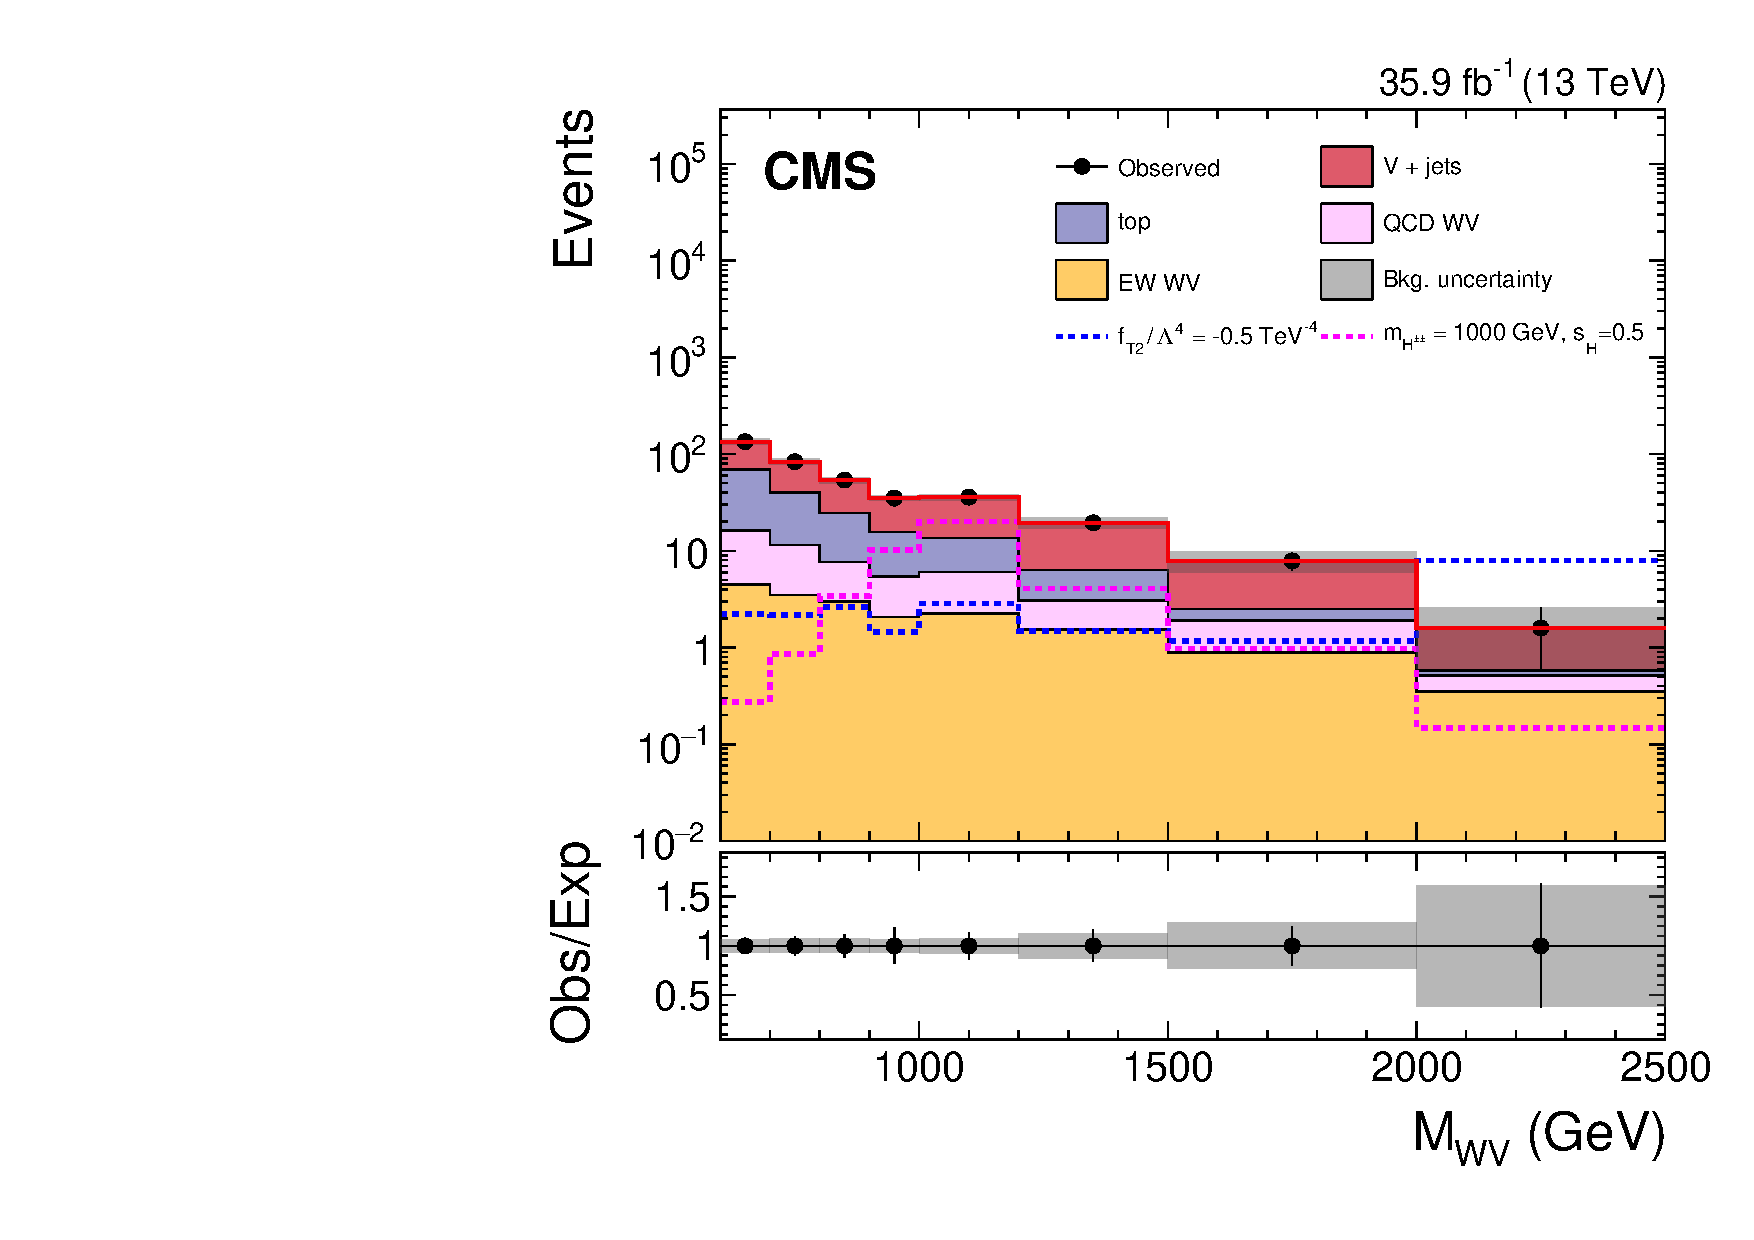
\includegraphics[width=0.45\textwidth]{Plots/plots/wv_signal.pdf}
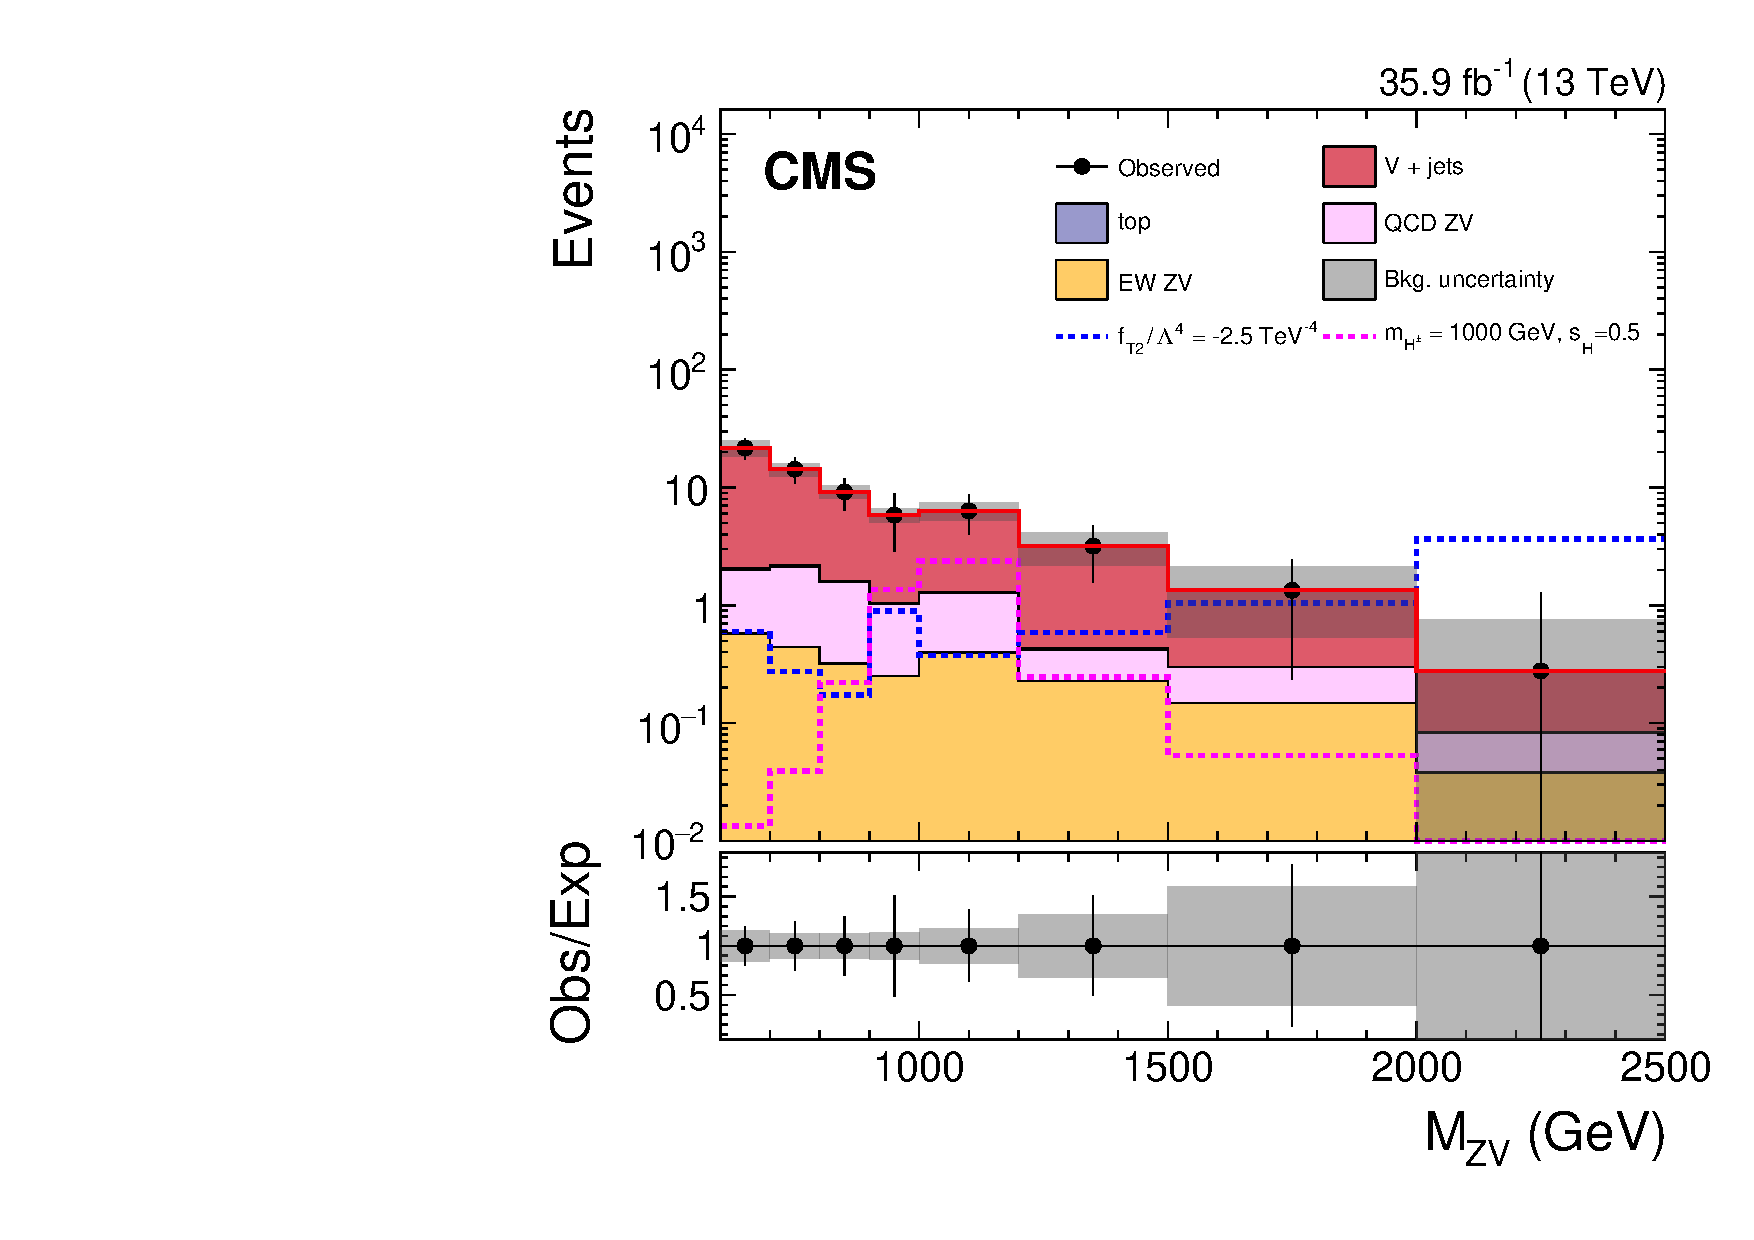
\includegraphics[width=0.45\textwidth]{Plots/plots/zv_signal.pdf}
\caption{Distributions of $m_{WV}$ (left) and $m_{ZV}$ (right) in the signal region. The gray bands include uncertainties from the predicted yields. The histograms for other backgrounds include the contributions from QCD initiated dibosons, top, $\PW+$jets, and Drell--Yan processes. The overflow is included in the last bin.The bottom inset in each figure shows the ratio of the number of events observed in data to that of the total background prediction.}
\label{fig:signal2}
\end{figure*}

\begin{table}[!htbp]
  \begin{center}
 % {\small
  \begin{tabular} {lccc}
  \hline
  \hline
  Final state 	& $\PW V$ &	& $\PZ V$ 	\\
  \cline{2-2} \cline{4-4}
  Data 	& 347 $\pm$ 16 && 47 $\pm$ 7 \\
  \hline
  $V+$jets    	      &   187 $\pm$ 21  &&    41.2 $\pm$ 6.1    \\
  top       	      &   120 $\pm$  18  &&    0.16 $\pm$  0.04    \\
  SM QCD VV  	      &   28 $\pm$  10  &&    6.4 $\pm$  2.2      \\
  SM EW VV  	      &   17 $\pm$  2  &&    2.4 $\pm$  0.4      \\
  \hline
  Total bkg.            &   352 $\pm$  21   &&    50.1 $\pm$  5.9   \\[1ex]
  $f_{T2}/ \Lambda^{4} = -0.5,-2.5~\TeV^{-4}$    &   22 $\pm$ 1 && 7.6 $\pm$ 0.6\\
  $m_{H}=500~\GeV$, $s_{h}=0.5$      &   40 $\pm$ 1 && 4.3 $\pm$ 0.1\\
  \hline
  \end{tabular}
% }
\caption{Expected yields from various background processes in $\PW V$ and $\PZ V$ final states. The statistical and systematic uncertainties are shown. The aQGC and charged higgs signal yields are also shown.}
\label{tab:sel_yields15}
  \end{center}
\end{table}
% section event_selection (end)


\section{Background Estimation} % (fold)
\label{sec:background_estimation}
A combination of data-driven methods and detailed simulated studies to 
estimate background contributions is used. In all cases where simulation is used, events are reweighted to correct for the pileup, lepton and trigger efficiencies to agree with the data distribution. The following background processes are considered: QCD initiated di-boson, top, $\PW+$jets, and Drell--Yan processes. 

\subsection{Diboson}
Simulation is used for estimating this process, as described in Section~\ref{sec:sample_used}. The expected contribution of this process in the signal region is small. The theoretical uncertainties in the prediction from variation of the renormalization and factorization scales are $35\%$. The uncertainty from the PDFs is $7\%$.

\subsection{Top}
Simulation is used for estimating this process, as described in Section~\ref{sec:sample_used}. The top background prediction is verified in a top enriched control region where the full signal selection is applied, except the b-tagging requirements are reverted. Figure~\ref{fig:top_control} shows the distributions of few kinematic variables in this control region. Normalization uncertainty of $10\%$ is assigned to the top background as good agreement between data and predictions is observed. 

\begin{figure*}[!htbp]
\centering
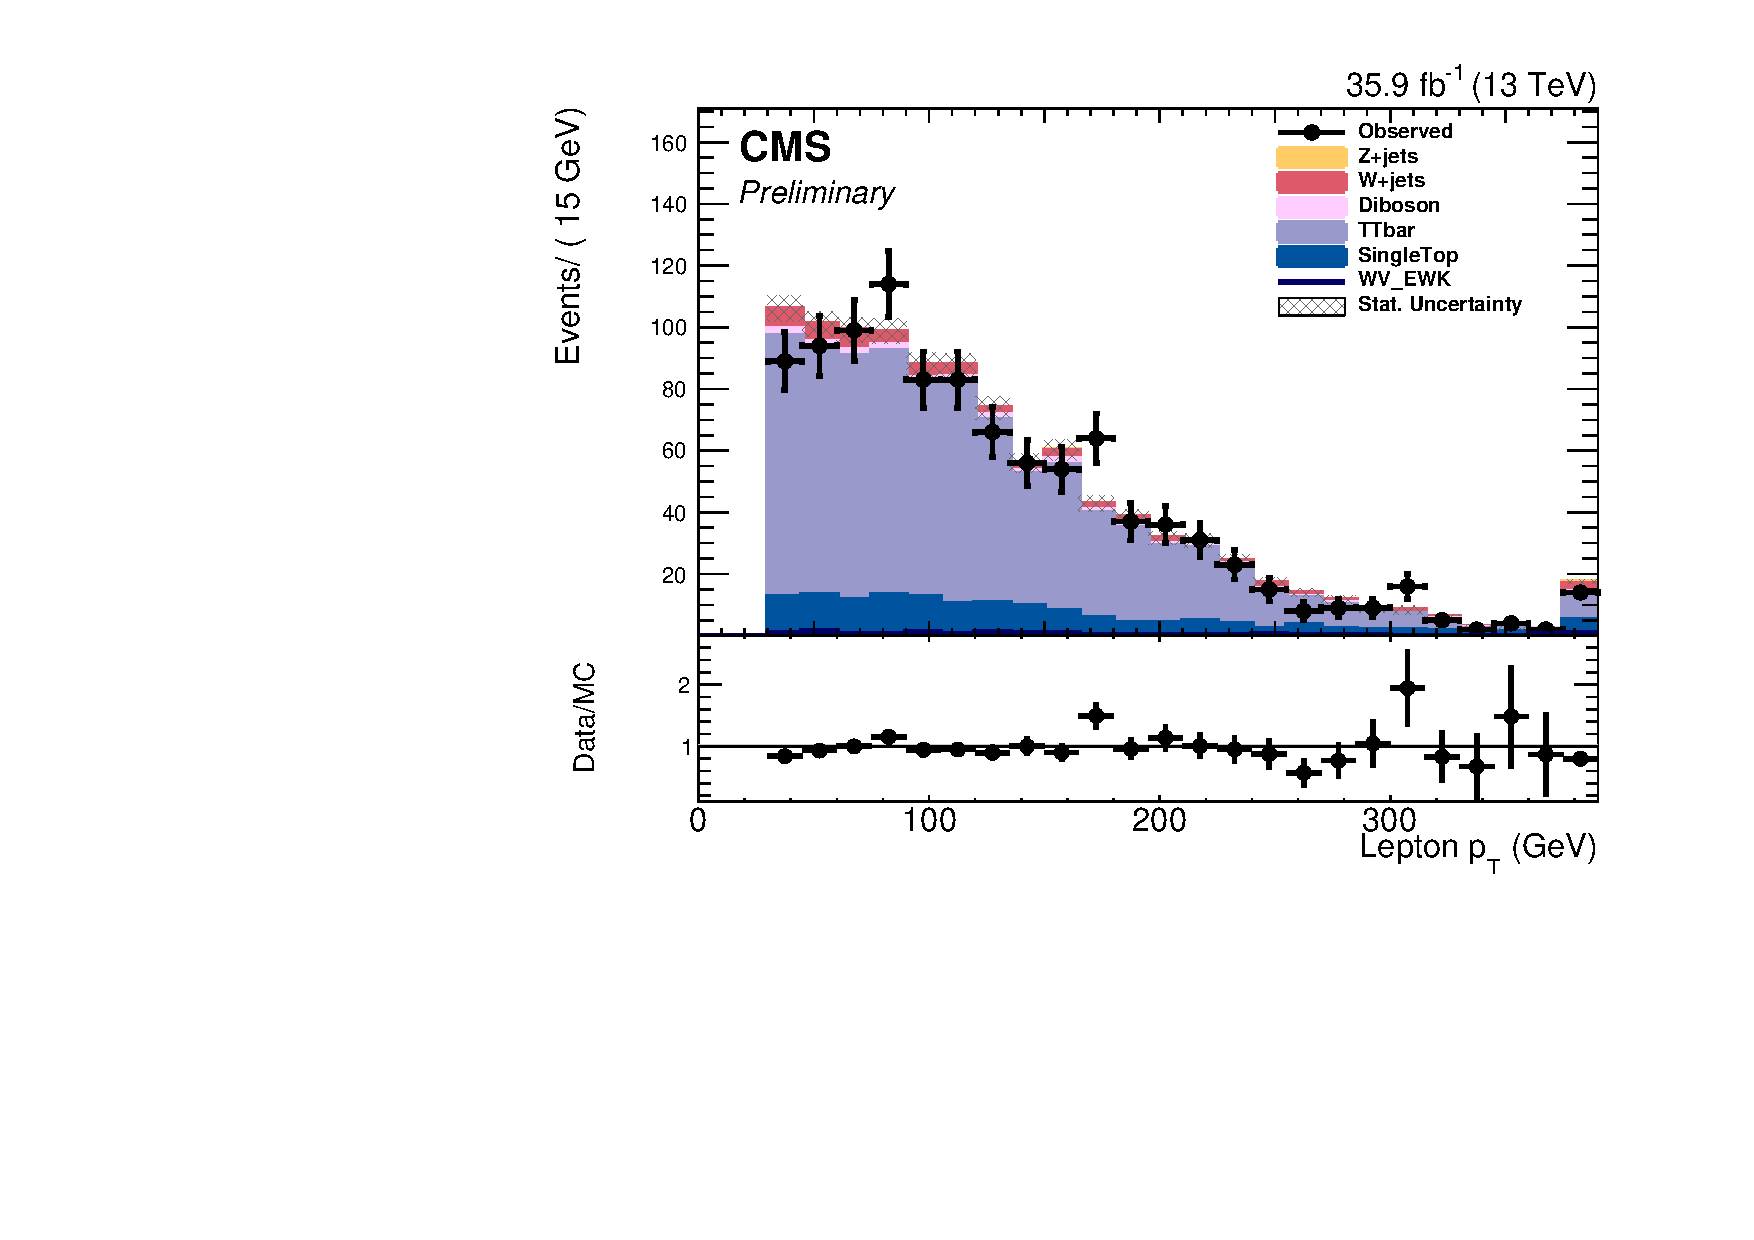
\includegraphics[width=0.45\textwidth]{Plots/plots/DibosonBoostedElMuCuts13TeV_TTBarControlRegion_CHS_lepton_pt.pdf}
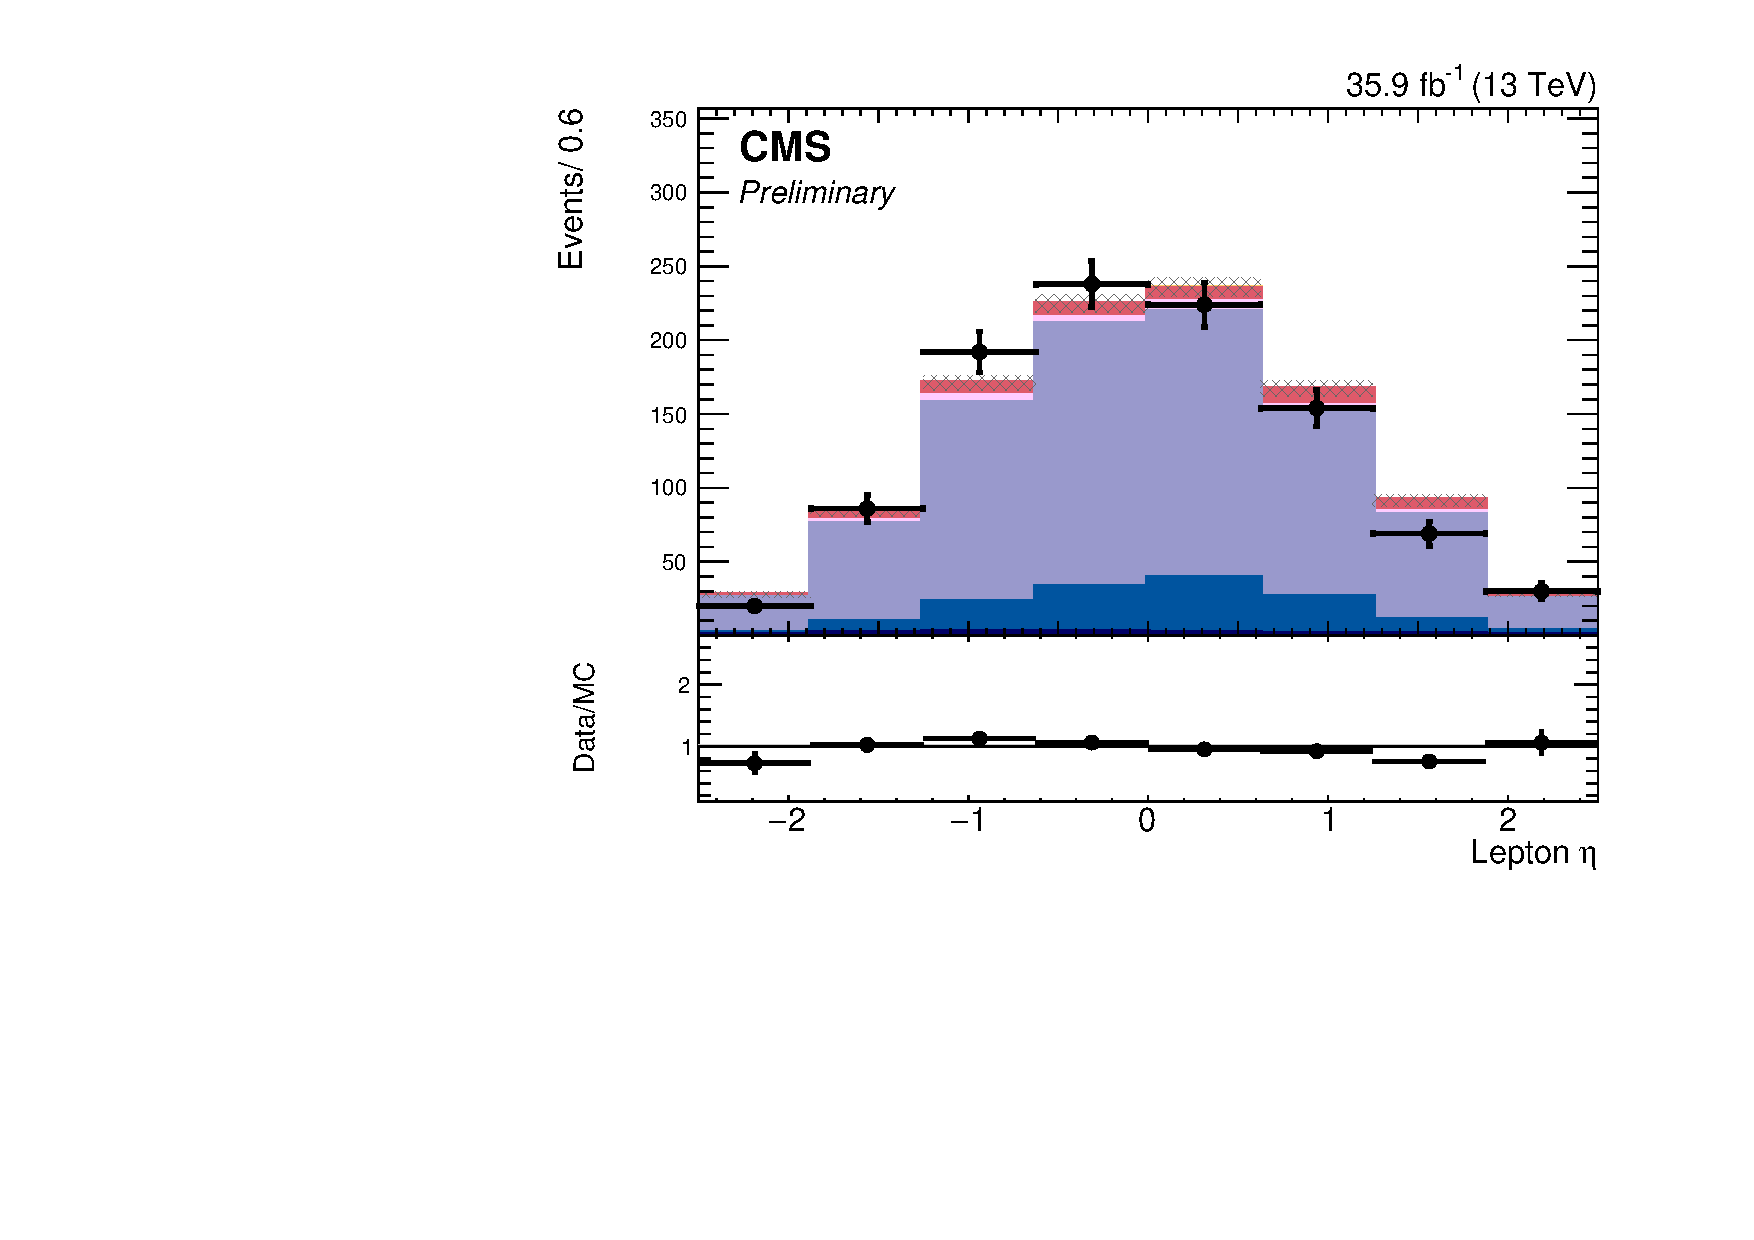
\includegraphics[width=0.45\textwidth]{Plots/plots/DibosonBoostedElMuCuts13TeV_TTBarControlRegion_CHS_lepton_eta.pdf}
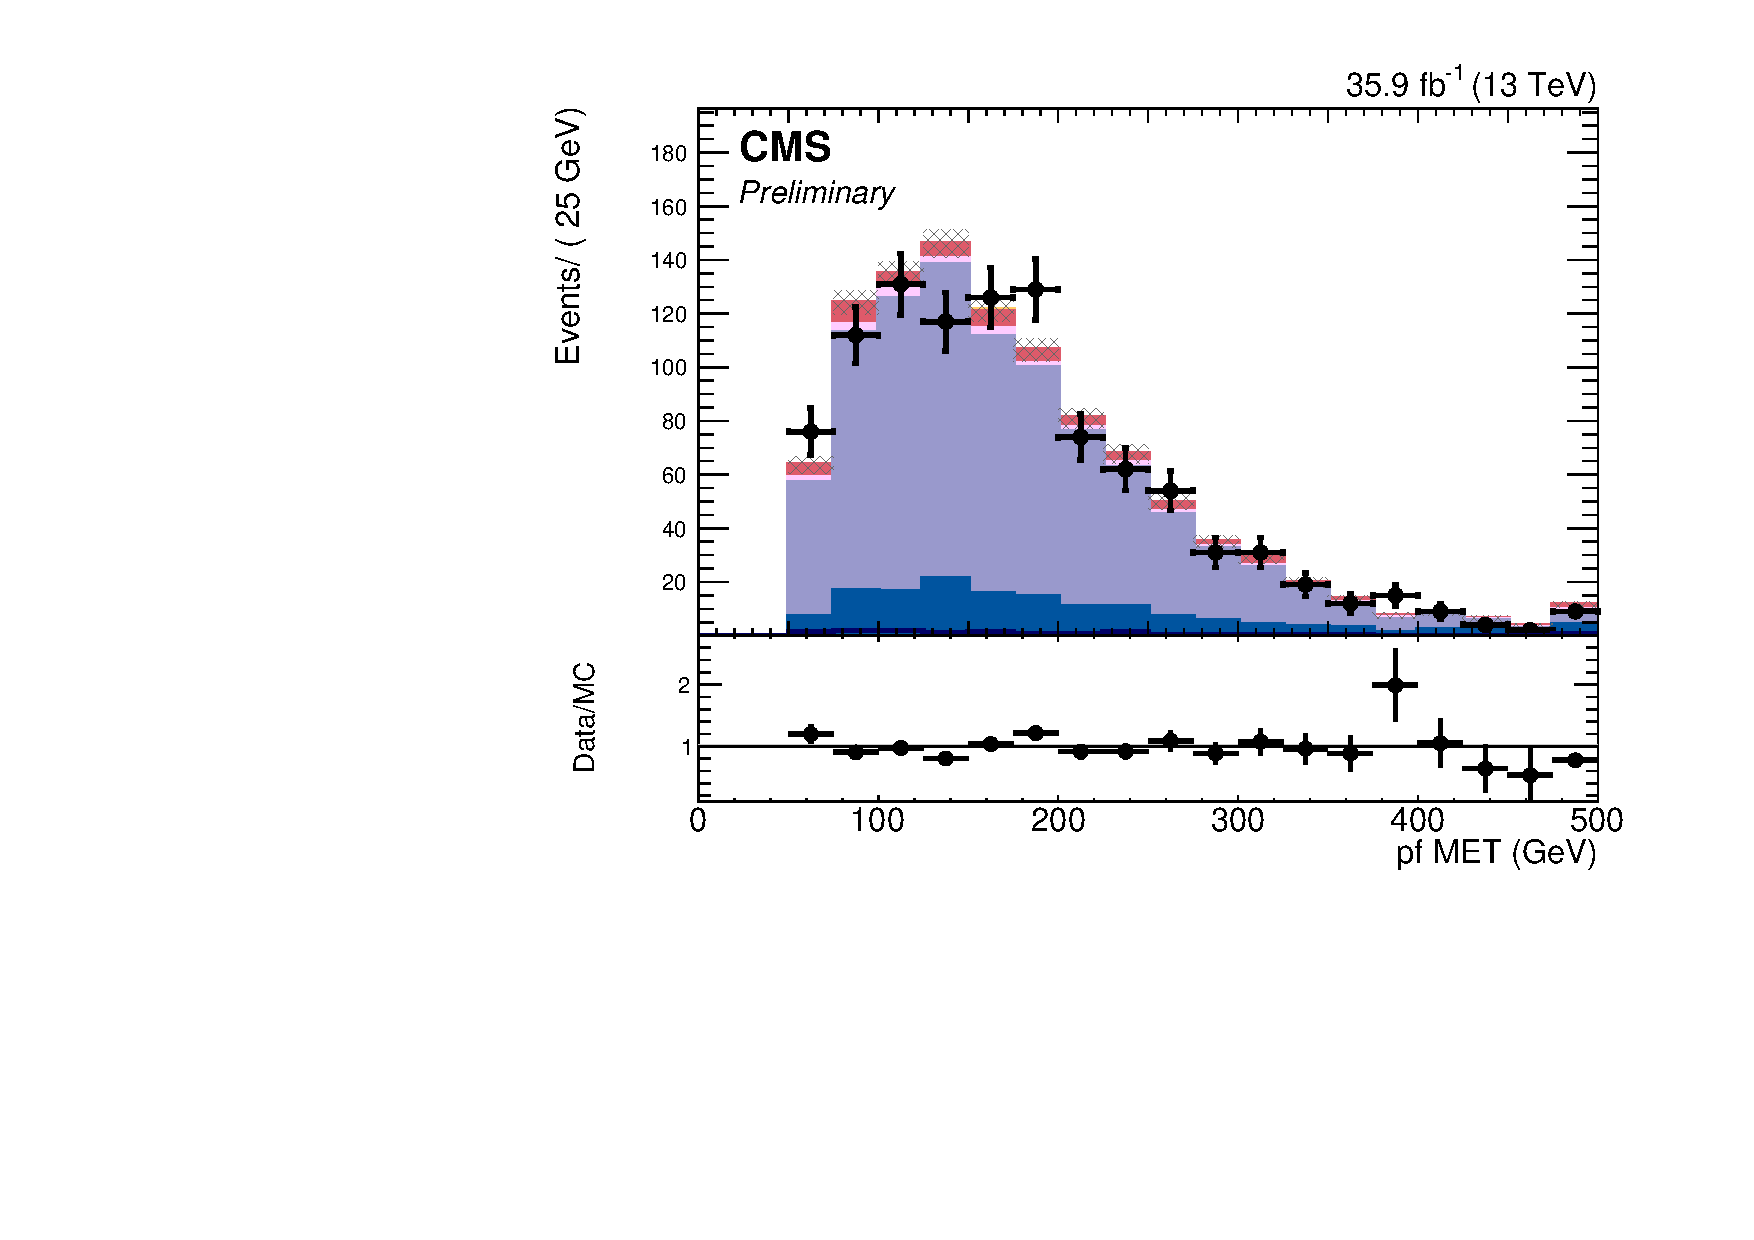
\includegraphics[width=0.45\textwidth]{Plots/plots/DibosonBoostedElMuCuts13TeV_TTBarControlRegion_CHS_pfMET_Corr.pdf}
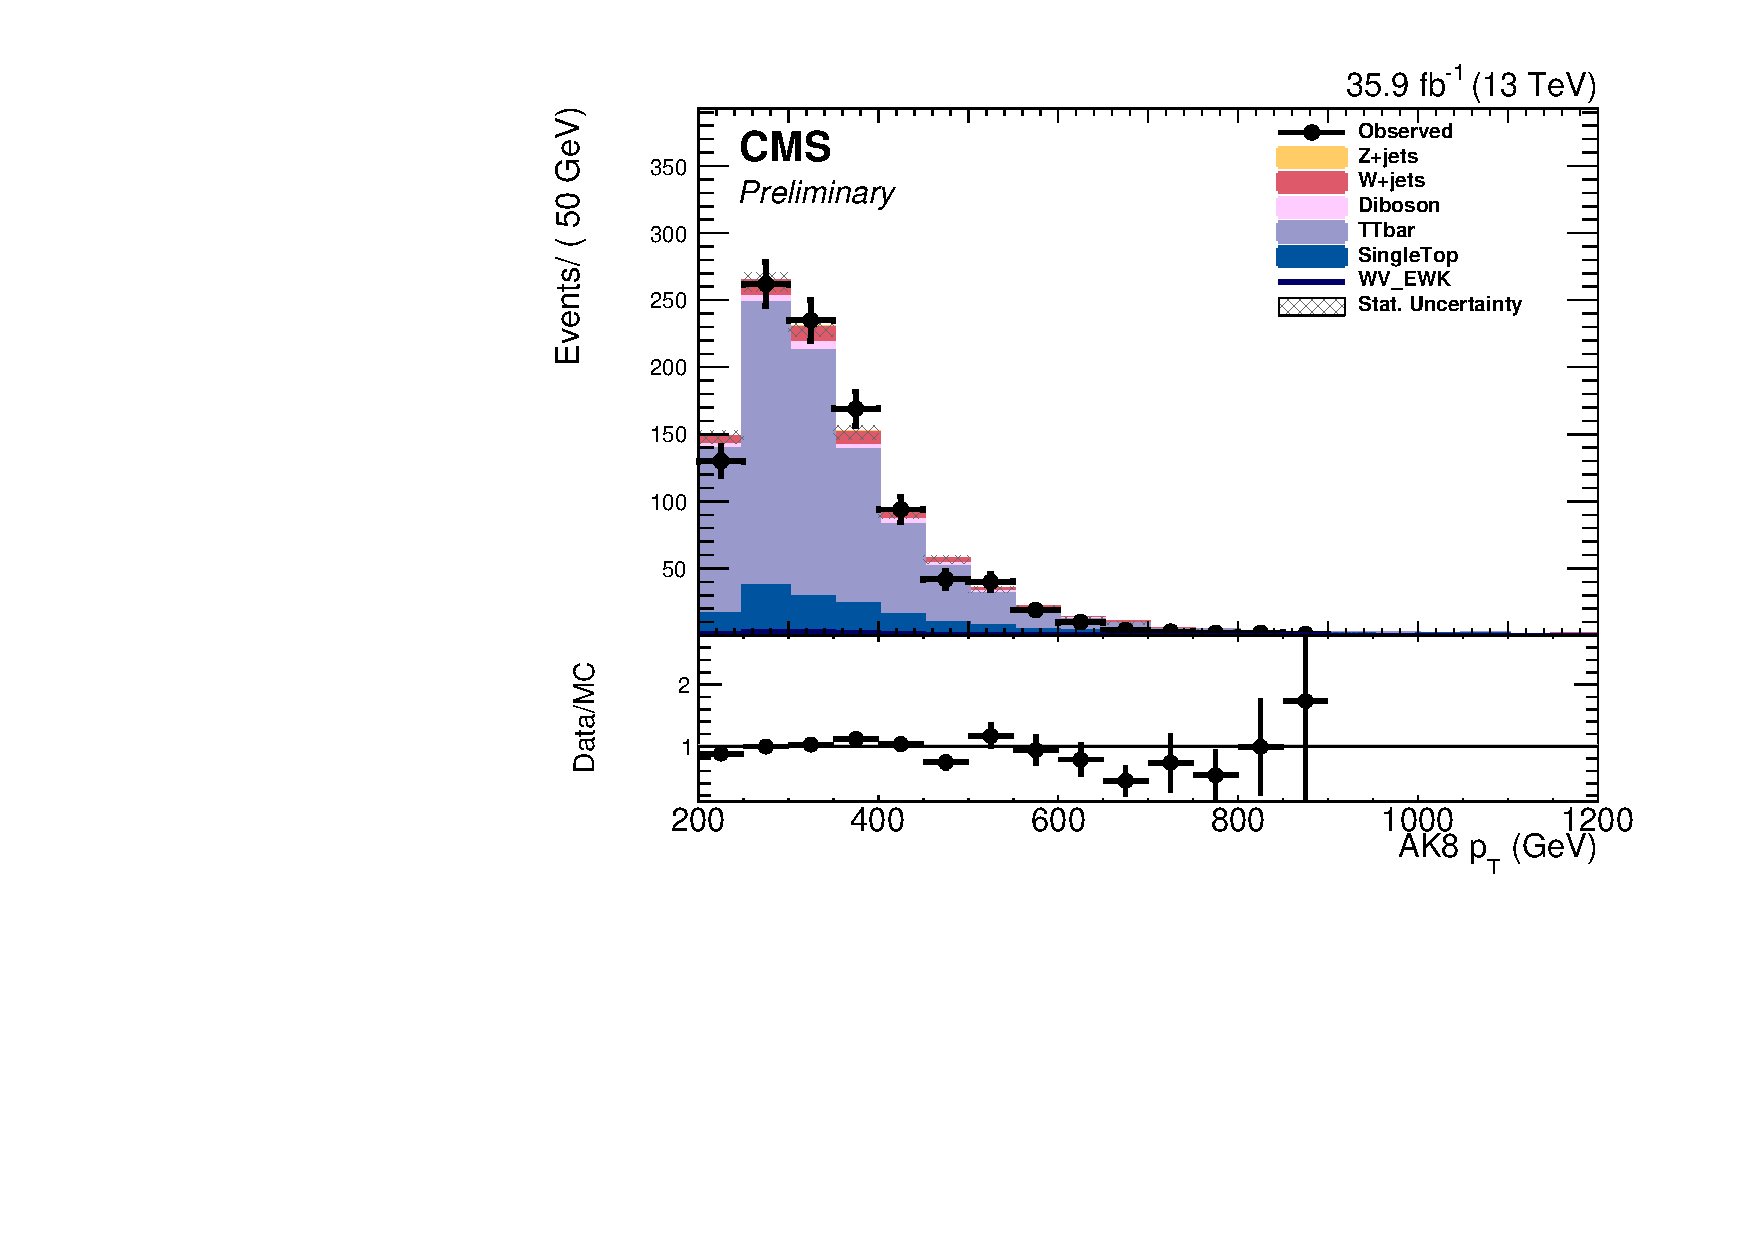
\includegraphics[width=0.45\textwidth]{Plots/plots/DibosonBoostedElMuCuts13TeV_TTBarControlRegion_CHS_ungroomed_PuppiAK8_jet_pt.pdf}
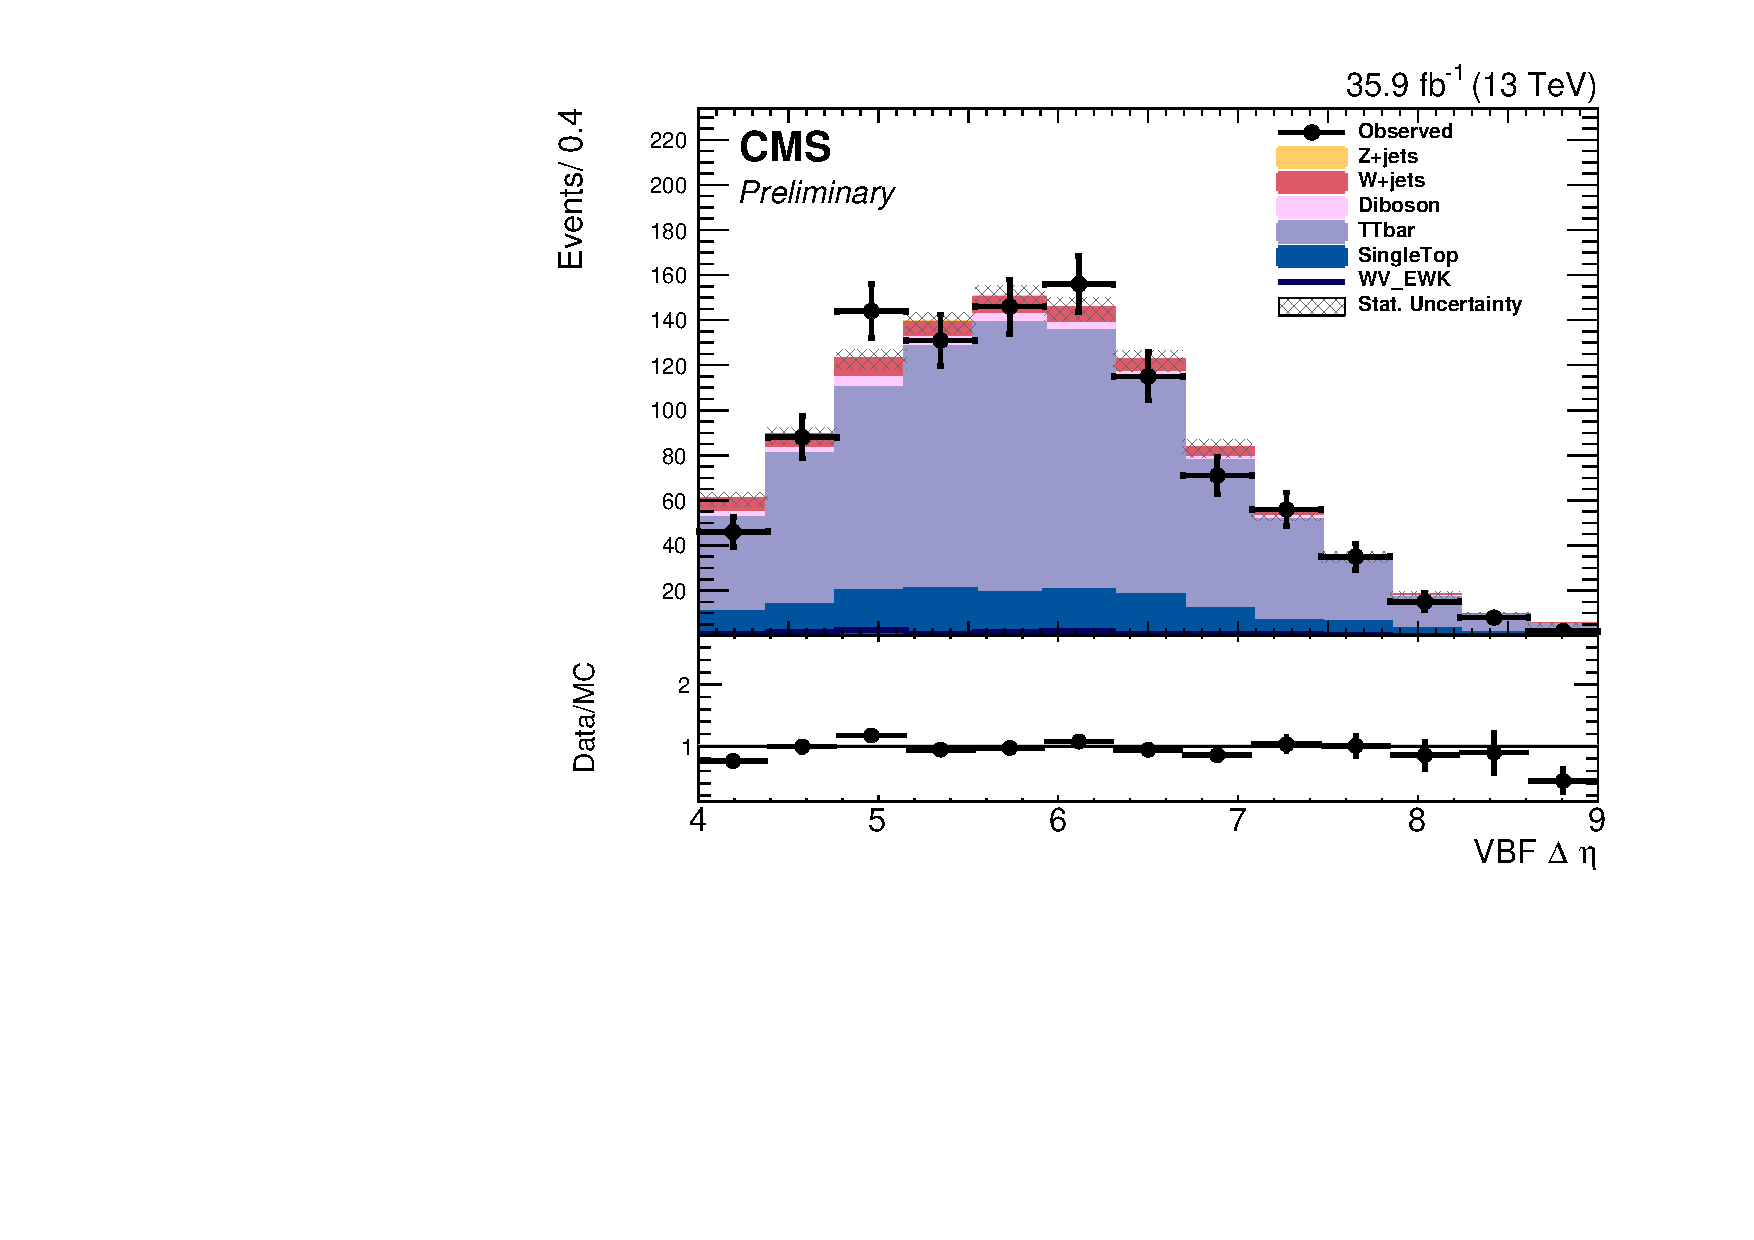
\includegraphics[width=0.45\textwidth]{Plots/plots/DibosonBoostedElMuCuts13TeV_TTBarControlRegion_CHS_vbf_maxpt_jj_Deta.pdf}
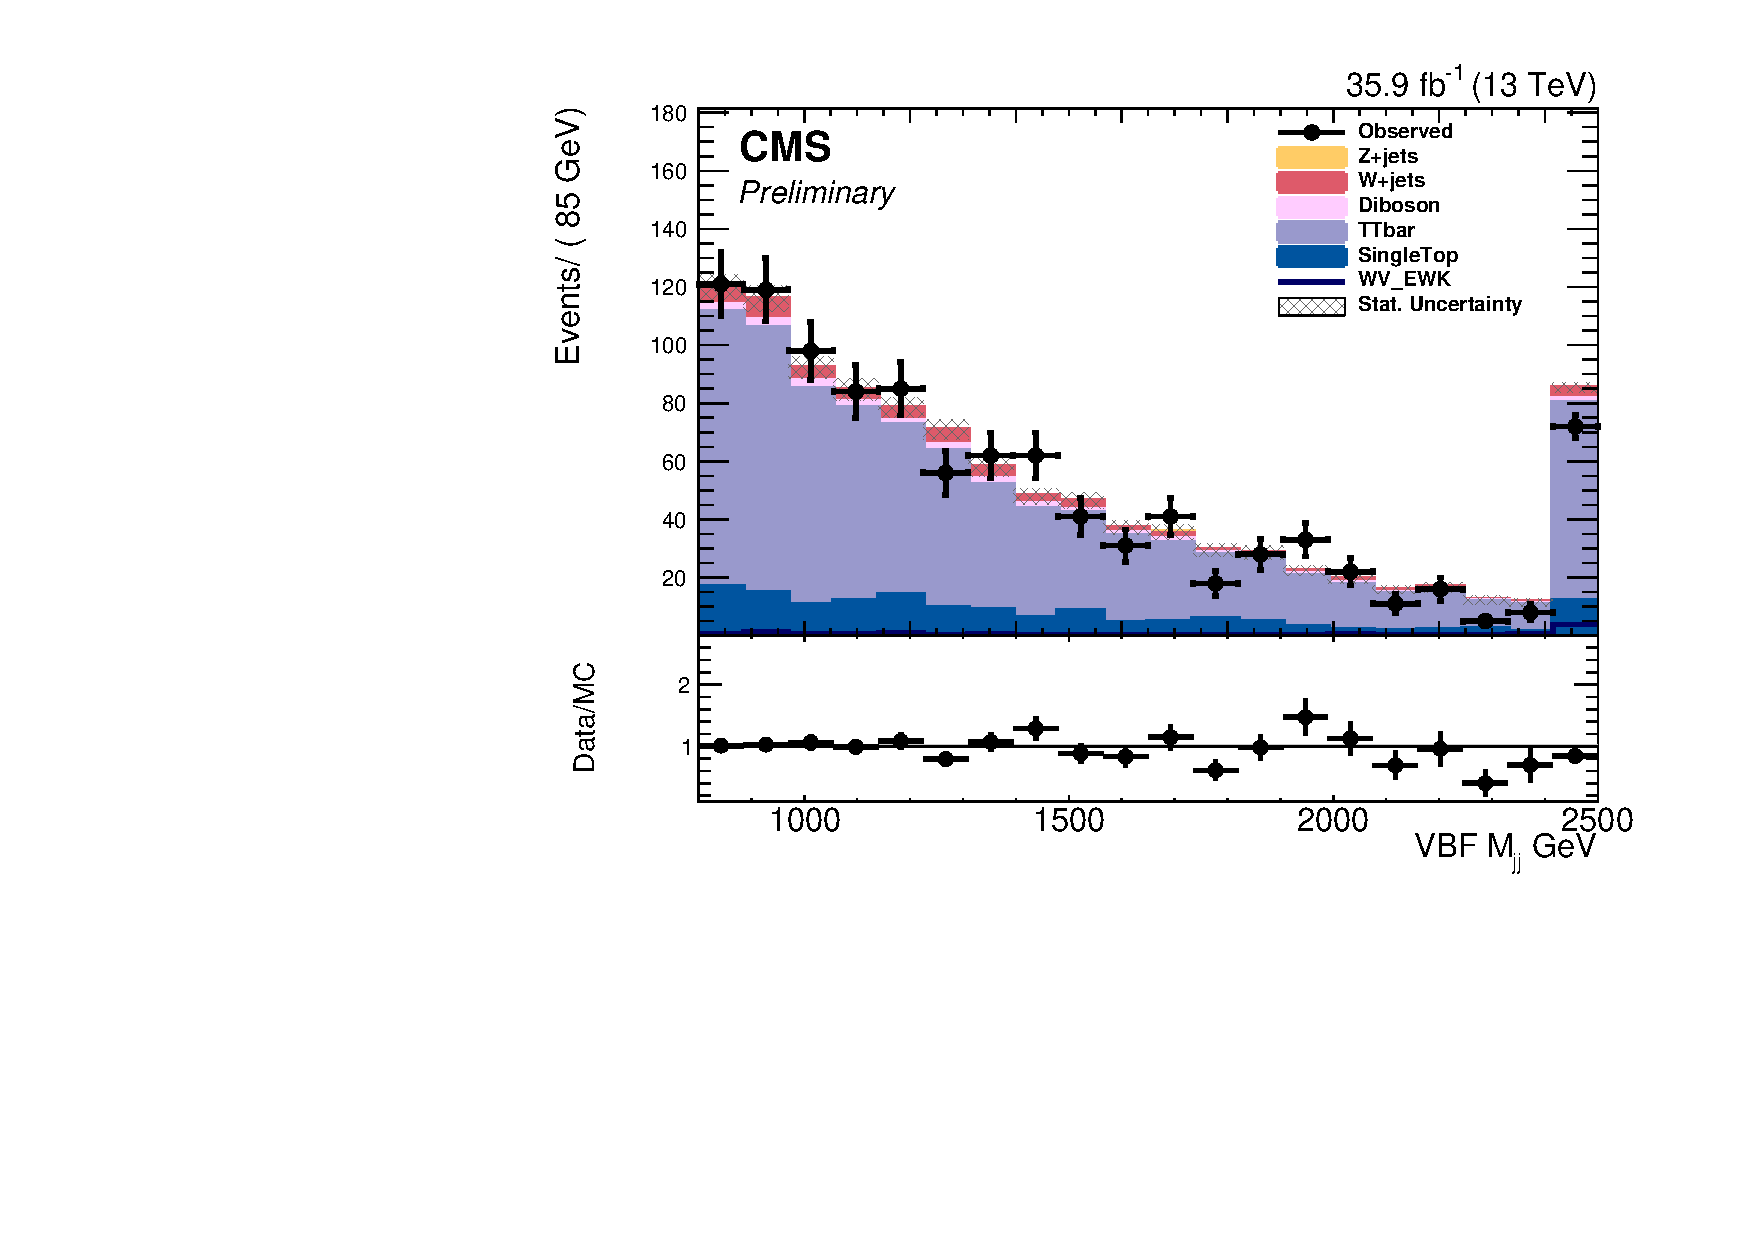
\includegraphics[width=0.45\textwidth]{Plots/plots/DibosonBoostedElMuCuts13TeV_TTBarControlRegion_CHS_vbf_maxpt_jj_m.pdf}
\caption{Kinematic distributions in the top background control region. The hatched bands include statistical uncertainties from the predicted yields.}
\label{fig:top_control}
\end{figure*}


\subsection{$\PW+$jets}
The $\PW+$jet background contribution is estimated from data using a $\PW+$jets enriched control region defined by selecting events with $40~\GeV < m_{V} < 65~\GeV$ or $105~\GeV < m_{V} < 150~\GeV$, where the full signal selection is applied. Figure~\ref{fig:wjet_control} shows the distributions of jet kinematic variables in this sideband region where $\PW+$jets predictions are taken from the simulation. Similarly, Figure~\ref{fig:wjet_control2} shows the distributions of the lepton, $\ptmiss$, and $V$ jet kinematic distributions. Generally good data-simulation agreement is seen. However, the $\PW+$jets MC sample is generated in $H_{T}$ bins at LO accuracy (see Table~\ref{tab:bkgSamples}). The number of available simulated events are not large enough for some $H_{T}$ bins resulting in large statistical uncertainties in the MC predictions. Therefore, the $\PW+$jets predictions from the simulation are not used in the statistical analysis of the event yields.

\begin{figure*}[!htbp]
\centering
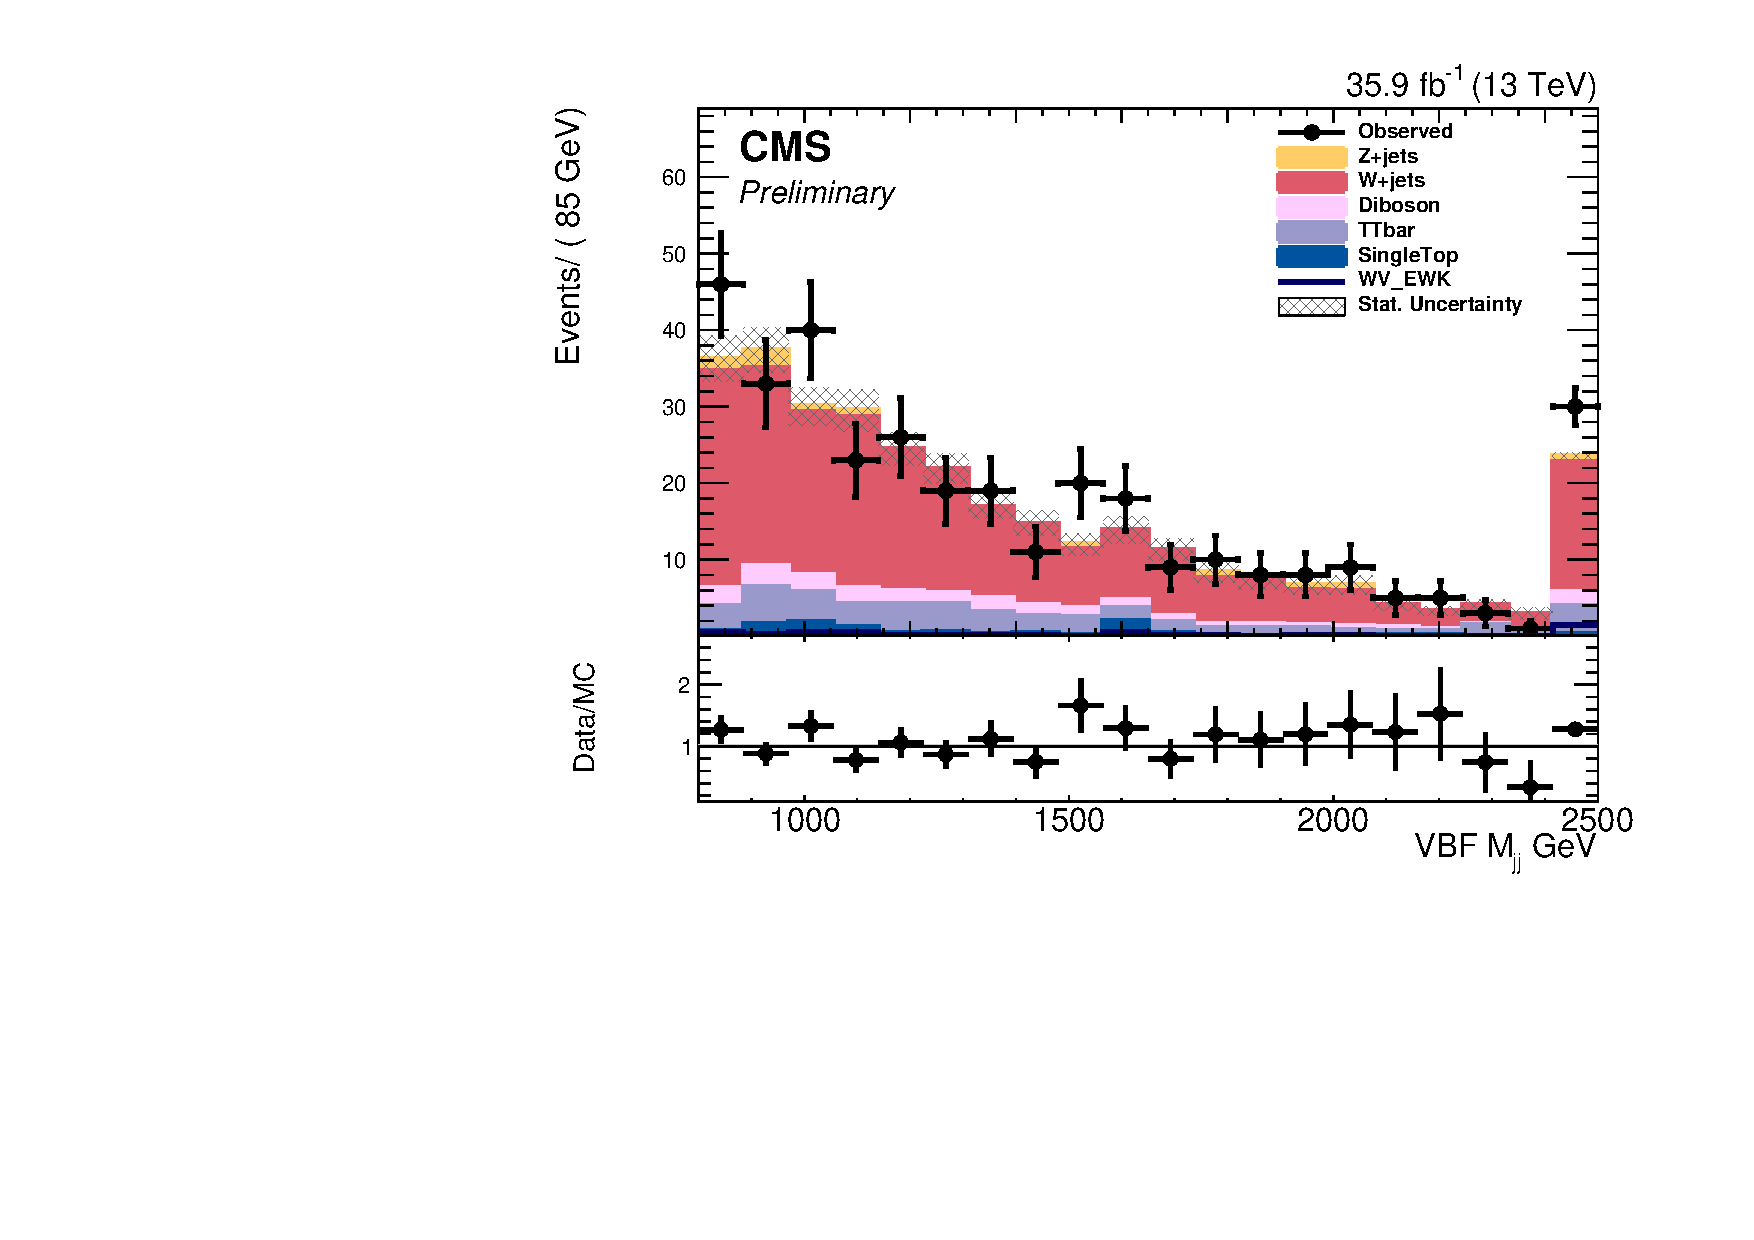
\includegraphics[width=0.45\textwidth]{Plots/plots/DibosonBoostedElMuCuts13TeV_WjetControlRegion_Tighter_CHS_vbf_maxpt_jj_m.pdf}
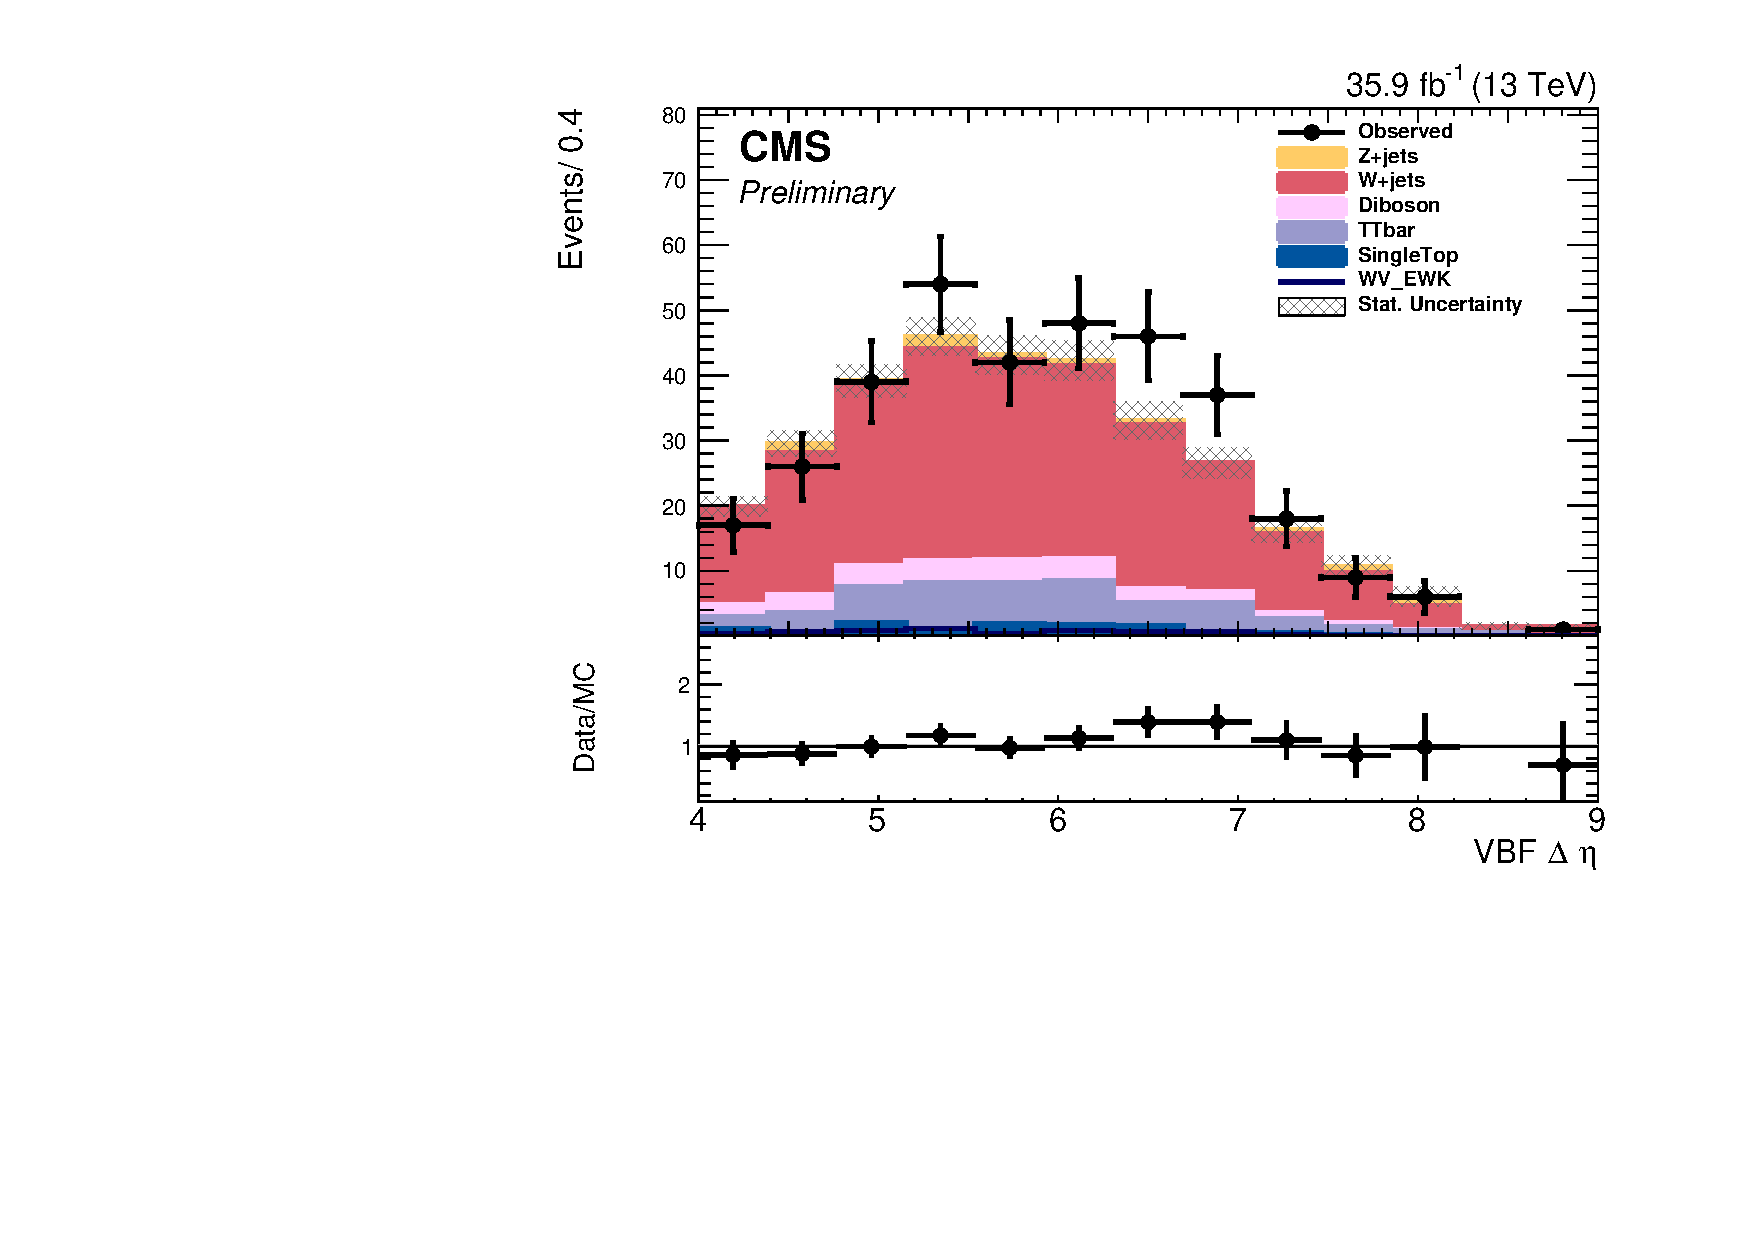
\includegraphics[width=0.45\textwidth]{Plots/plots/DibosonBoostedElMuCuts13TeV_WjetControlRegion_Tighter_CHS_vbf_maxpt_jj_Deta.pdf}
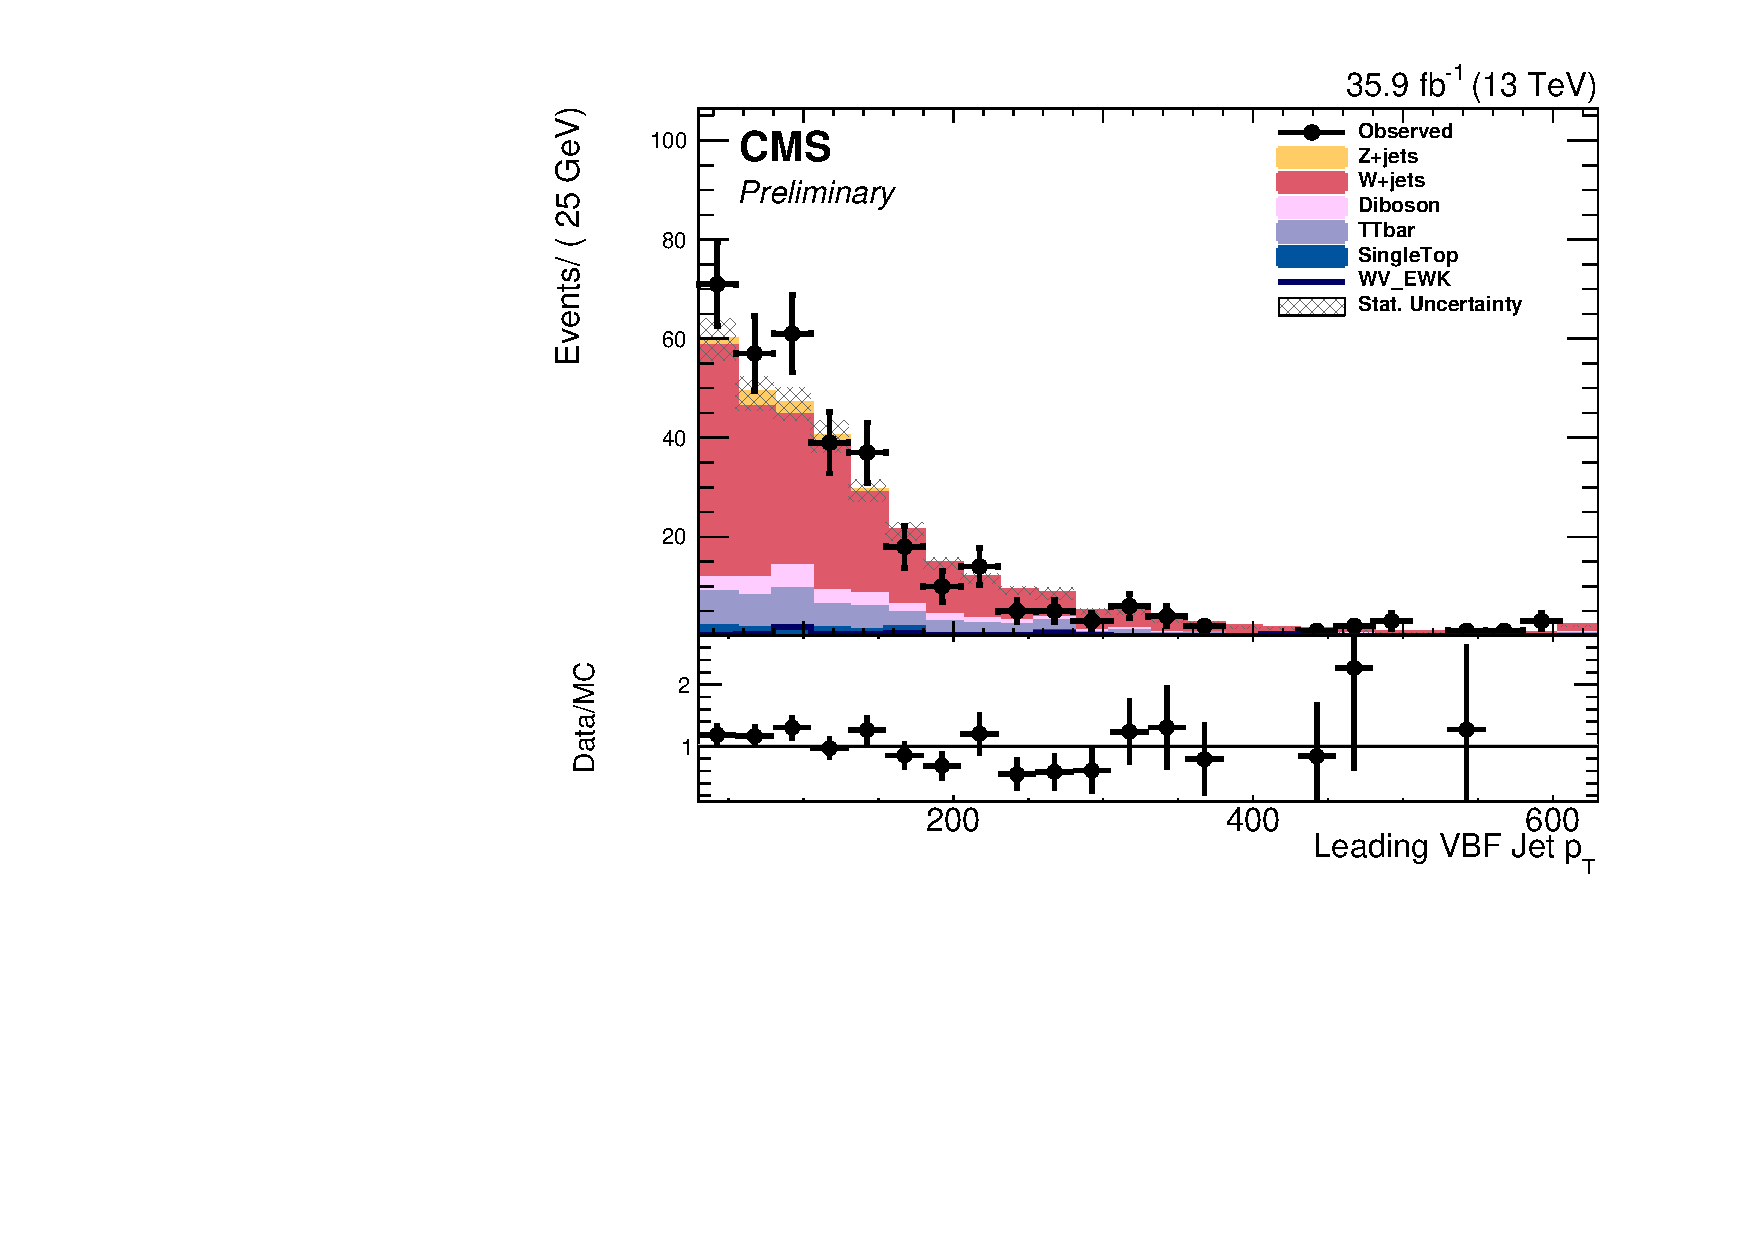
\includegraphics[width=0.45\textwidth]{Plots/plots/DibosonBoostedElMuCuts13TeV_WjetControlRegion_Tighter_CHS_vbf_maxpt_j1_pt.pdf}
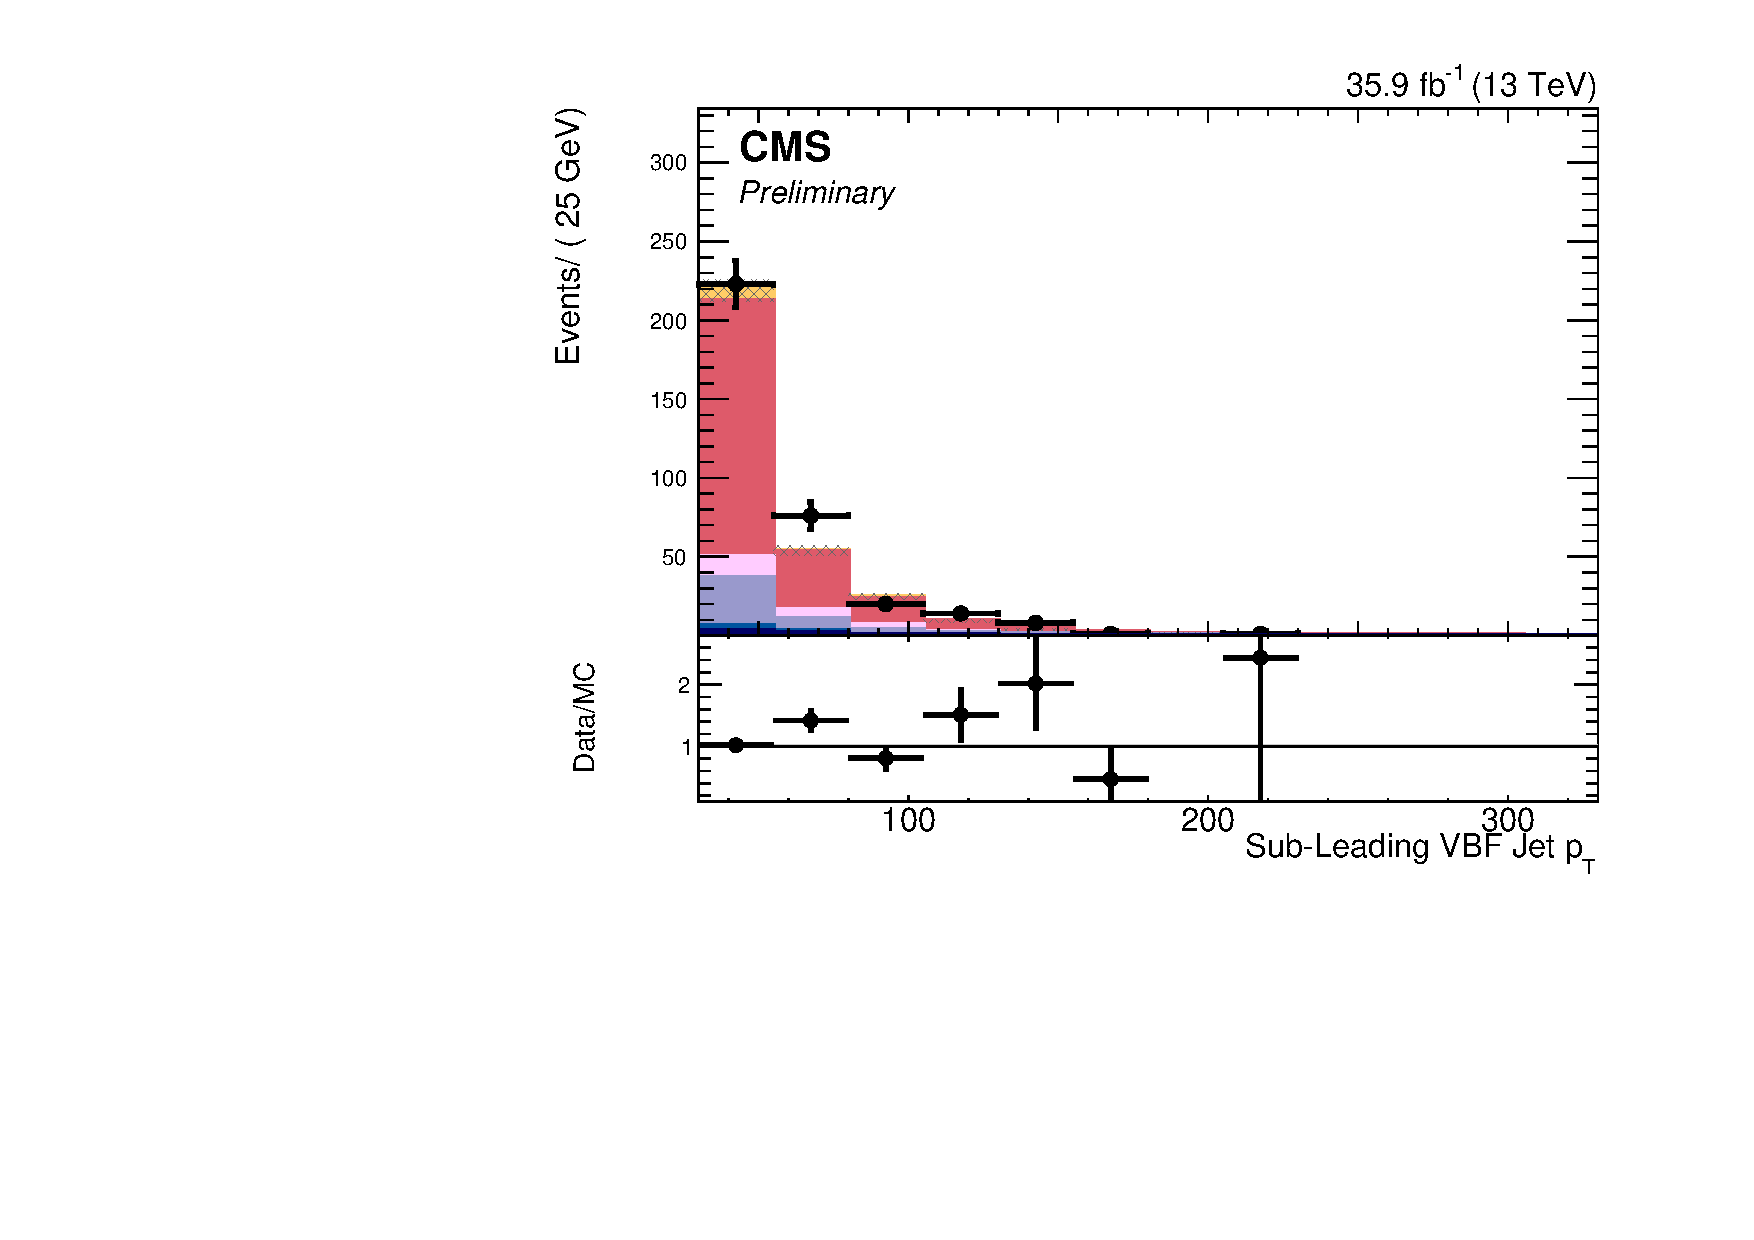
\includegraphics[width=0.45\textwidth]{Plots/plots/DibosonBoostedElMuCuts13TeV_WjetControlRegion_Tighter_CHS_vbf_maxpt_j2_pt.pdf}
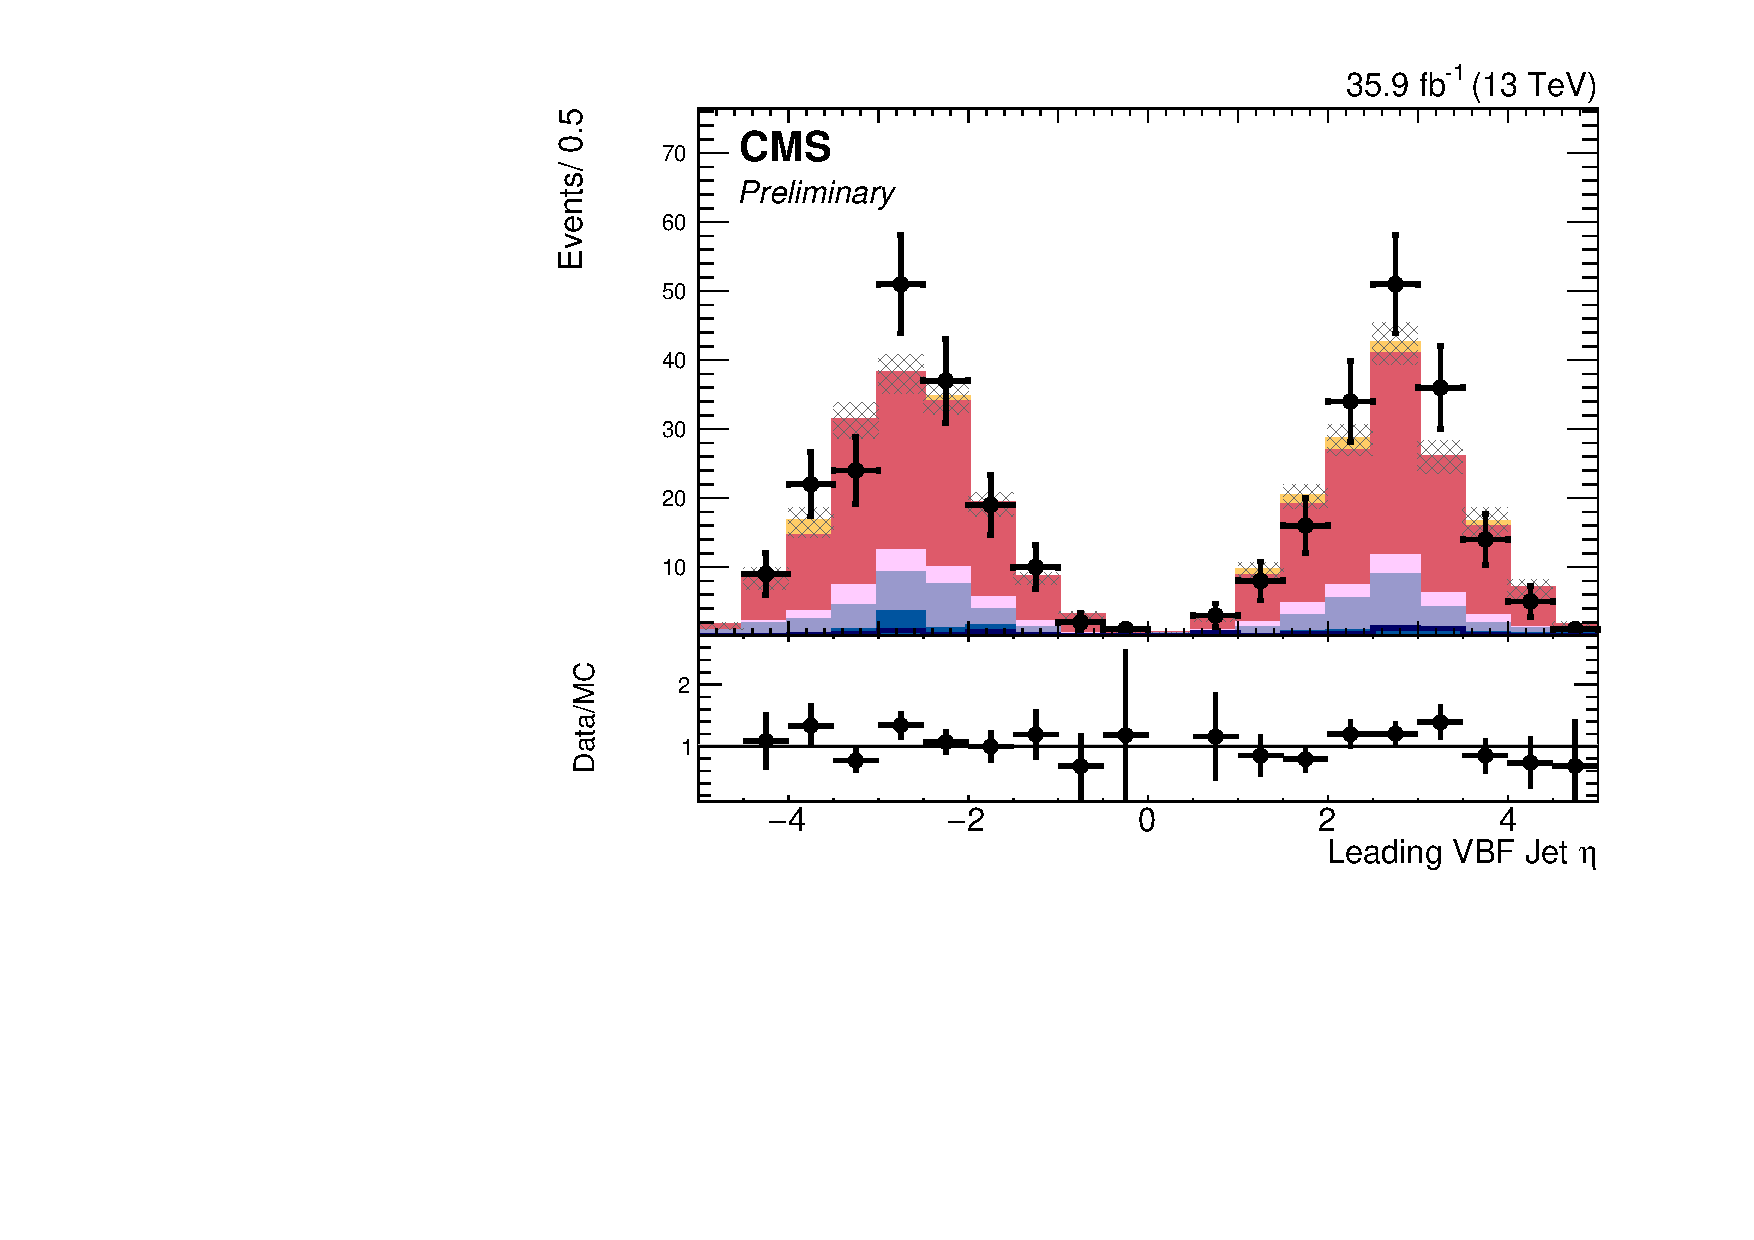
\includegraphics[width=0.45\textwidth]{Plots/plots/DibosonBoostedElMuCuts13TeV_WjetControlRegion_Tighter_CHS_vbf_maxpt_j1_eta.pdf}
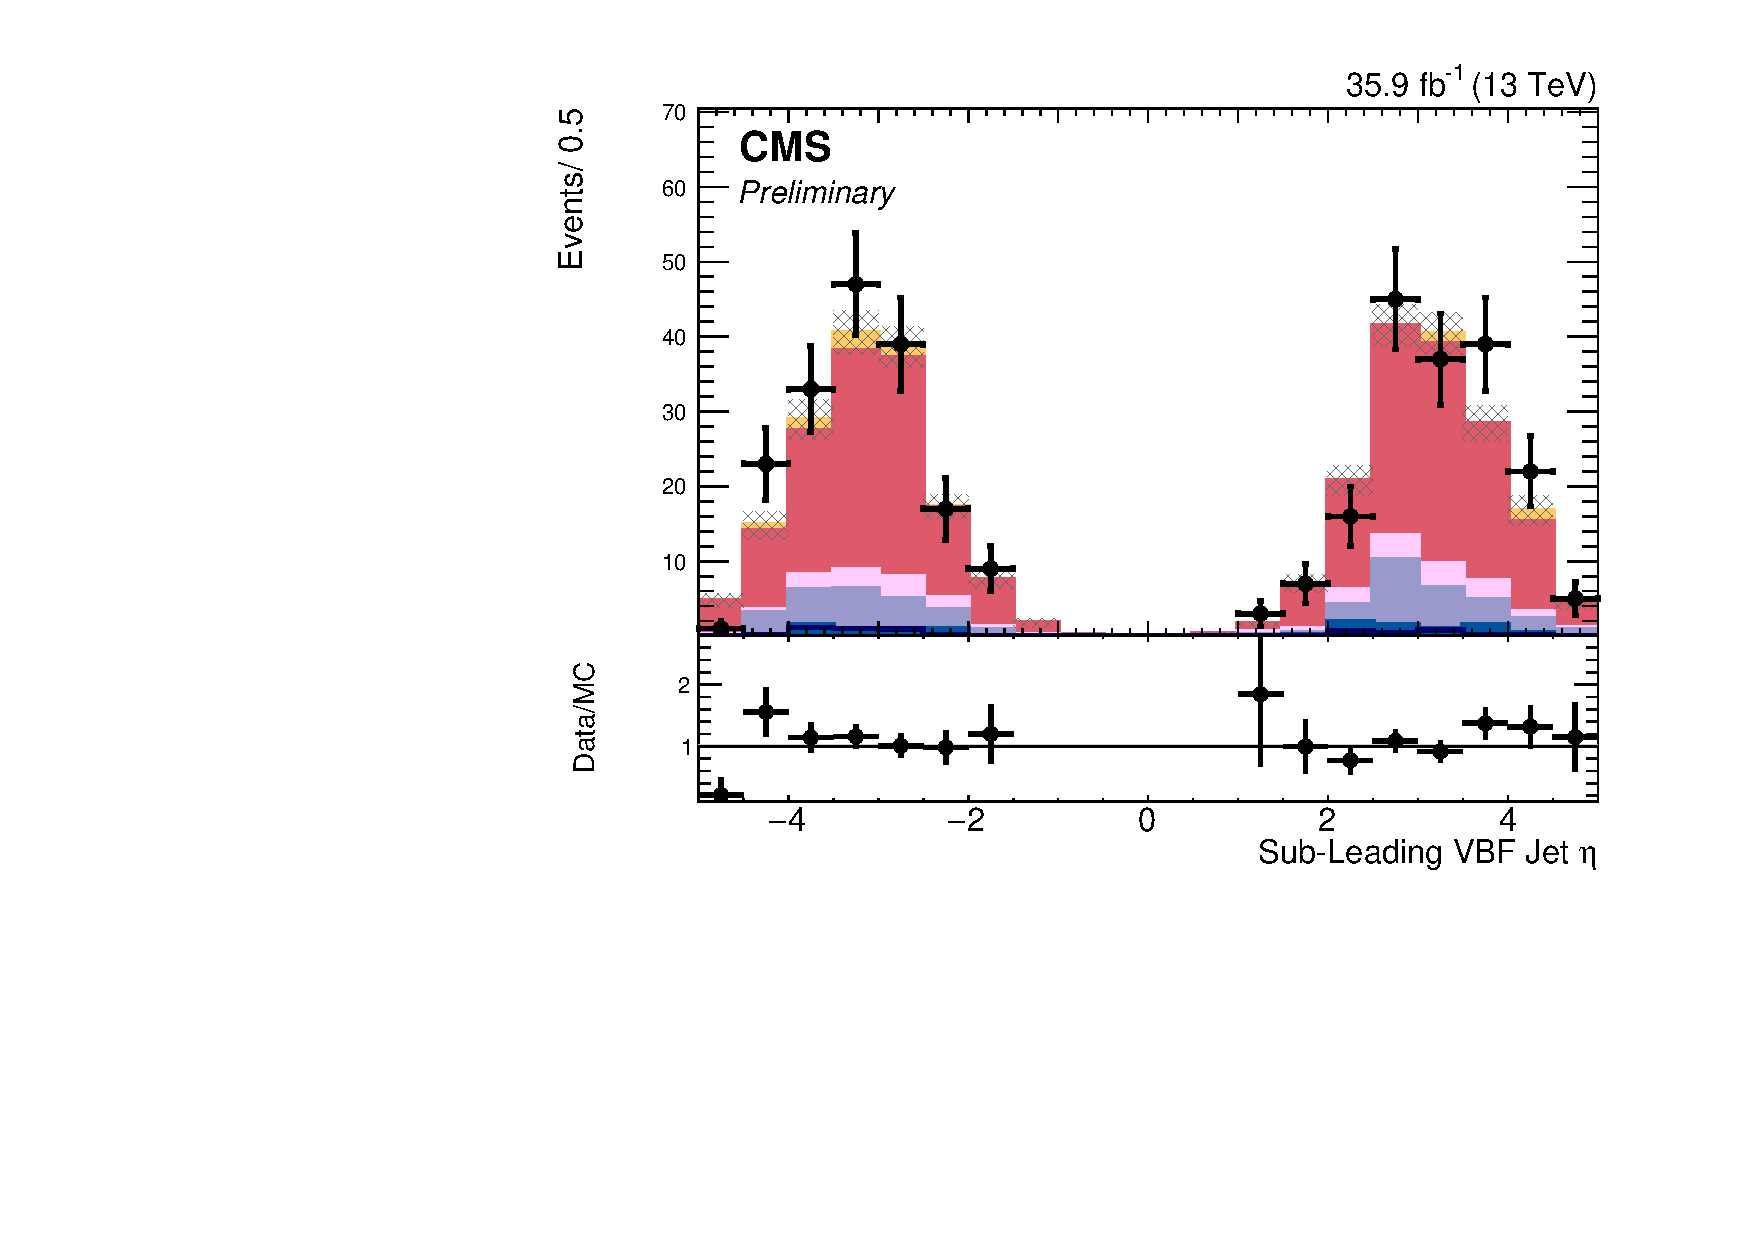
\includegraphics[width=0.45\textwidth]{Plots/plots/DibosonBoostedElMuCuts13TeV_WjetControlRegion_Tighter_CHS_vbf_maxpt_j2_eta.pdf}
\caption{Kinematic distributions in the $\PW+$jets background sideband region. $\PW+$jets predictions are taken from the simulation. The hatched bands include statistical uncertainties from the predicted yields.}
\label{fig:wjet_control}
\end{figure*}
 
\begin{figure*}[!htbp]
\centering
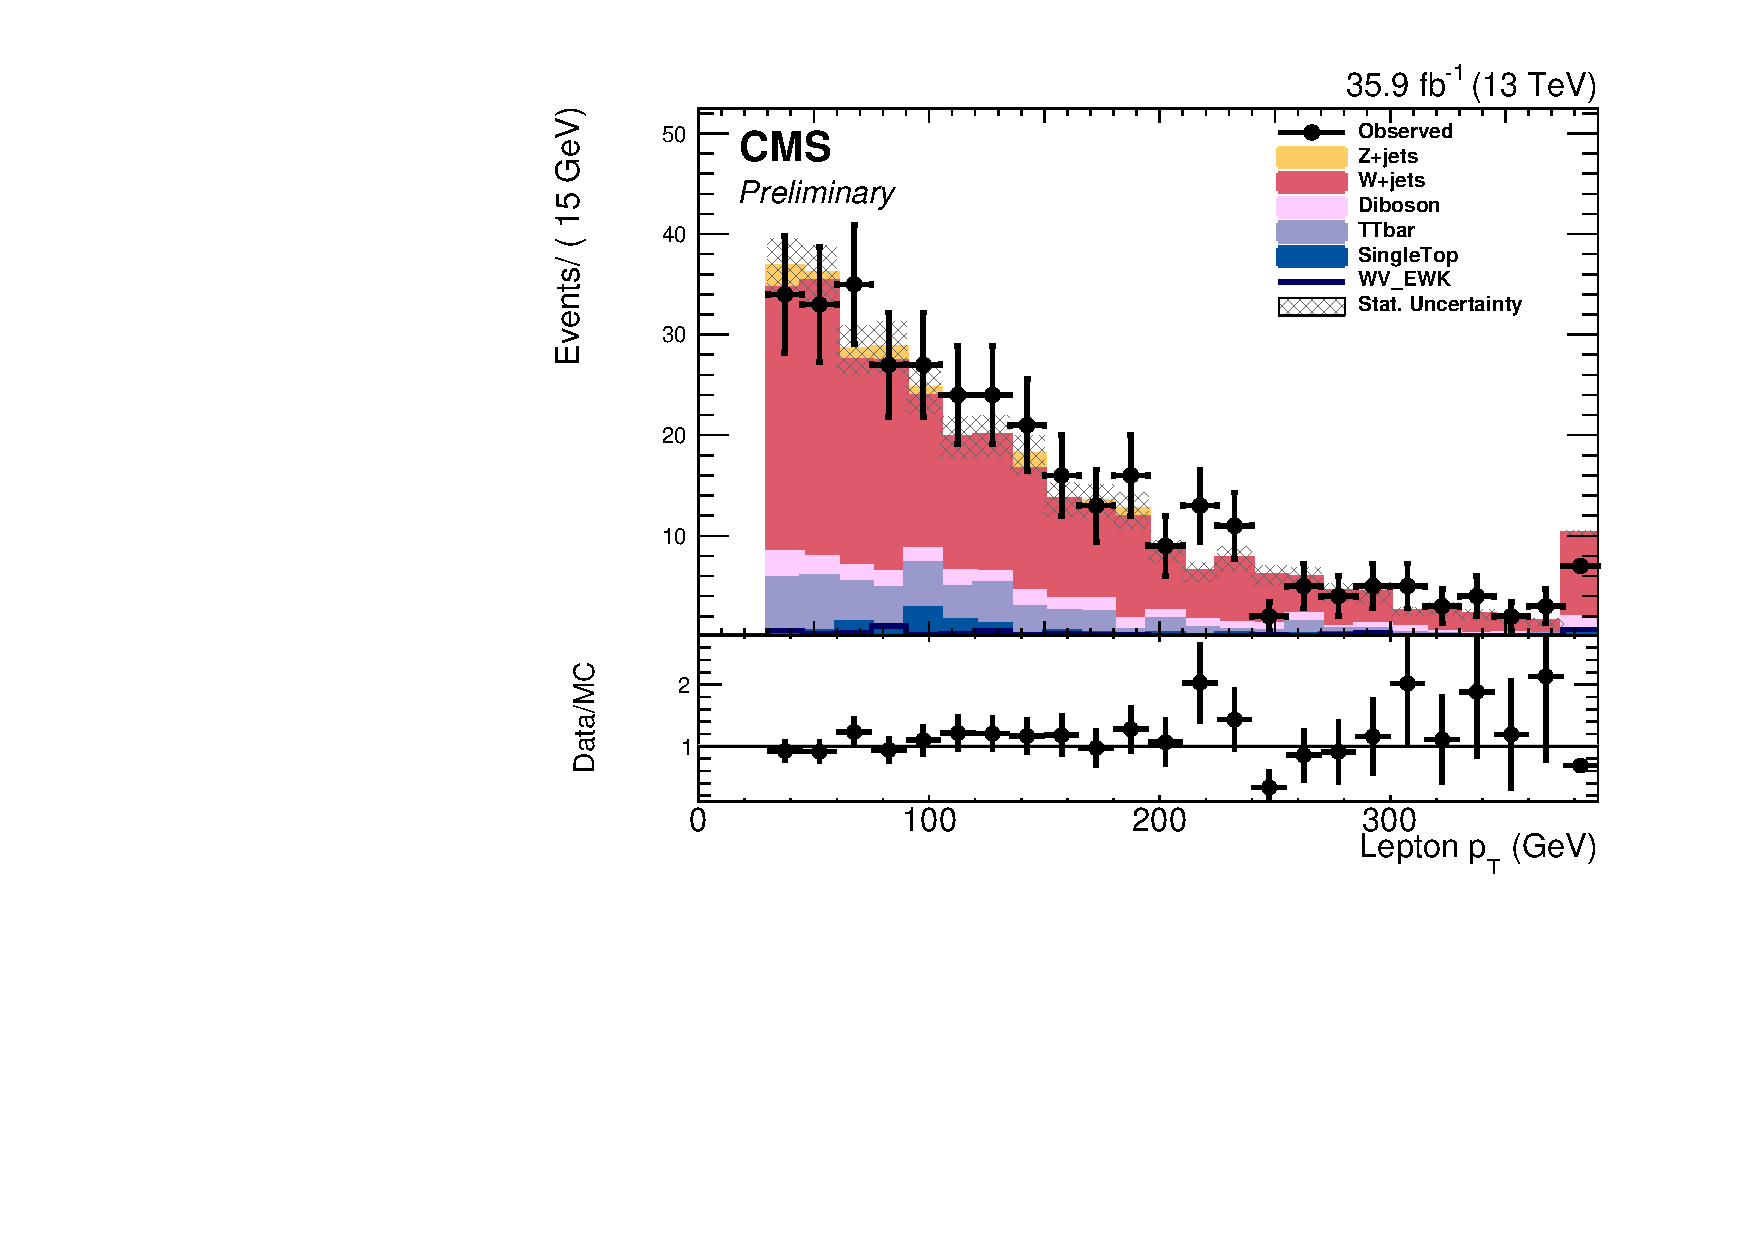
\includegraphics[width=0.45\textwidth]{Plots/plots/DibosonBoostedElMuCuts13TeV_WjetControlRegion_Tighter_CHS_lepton_pt.pdf}
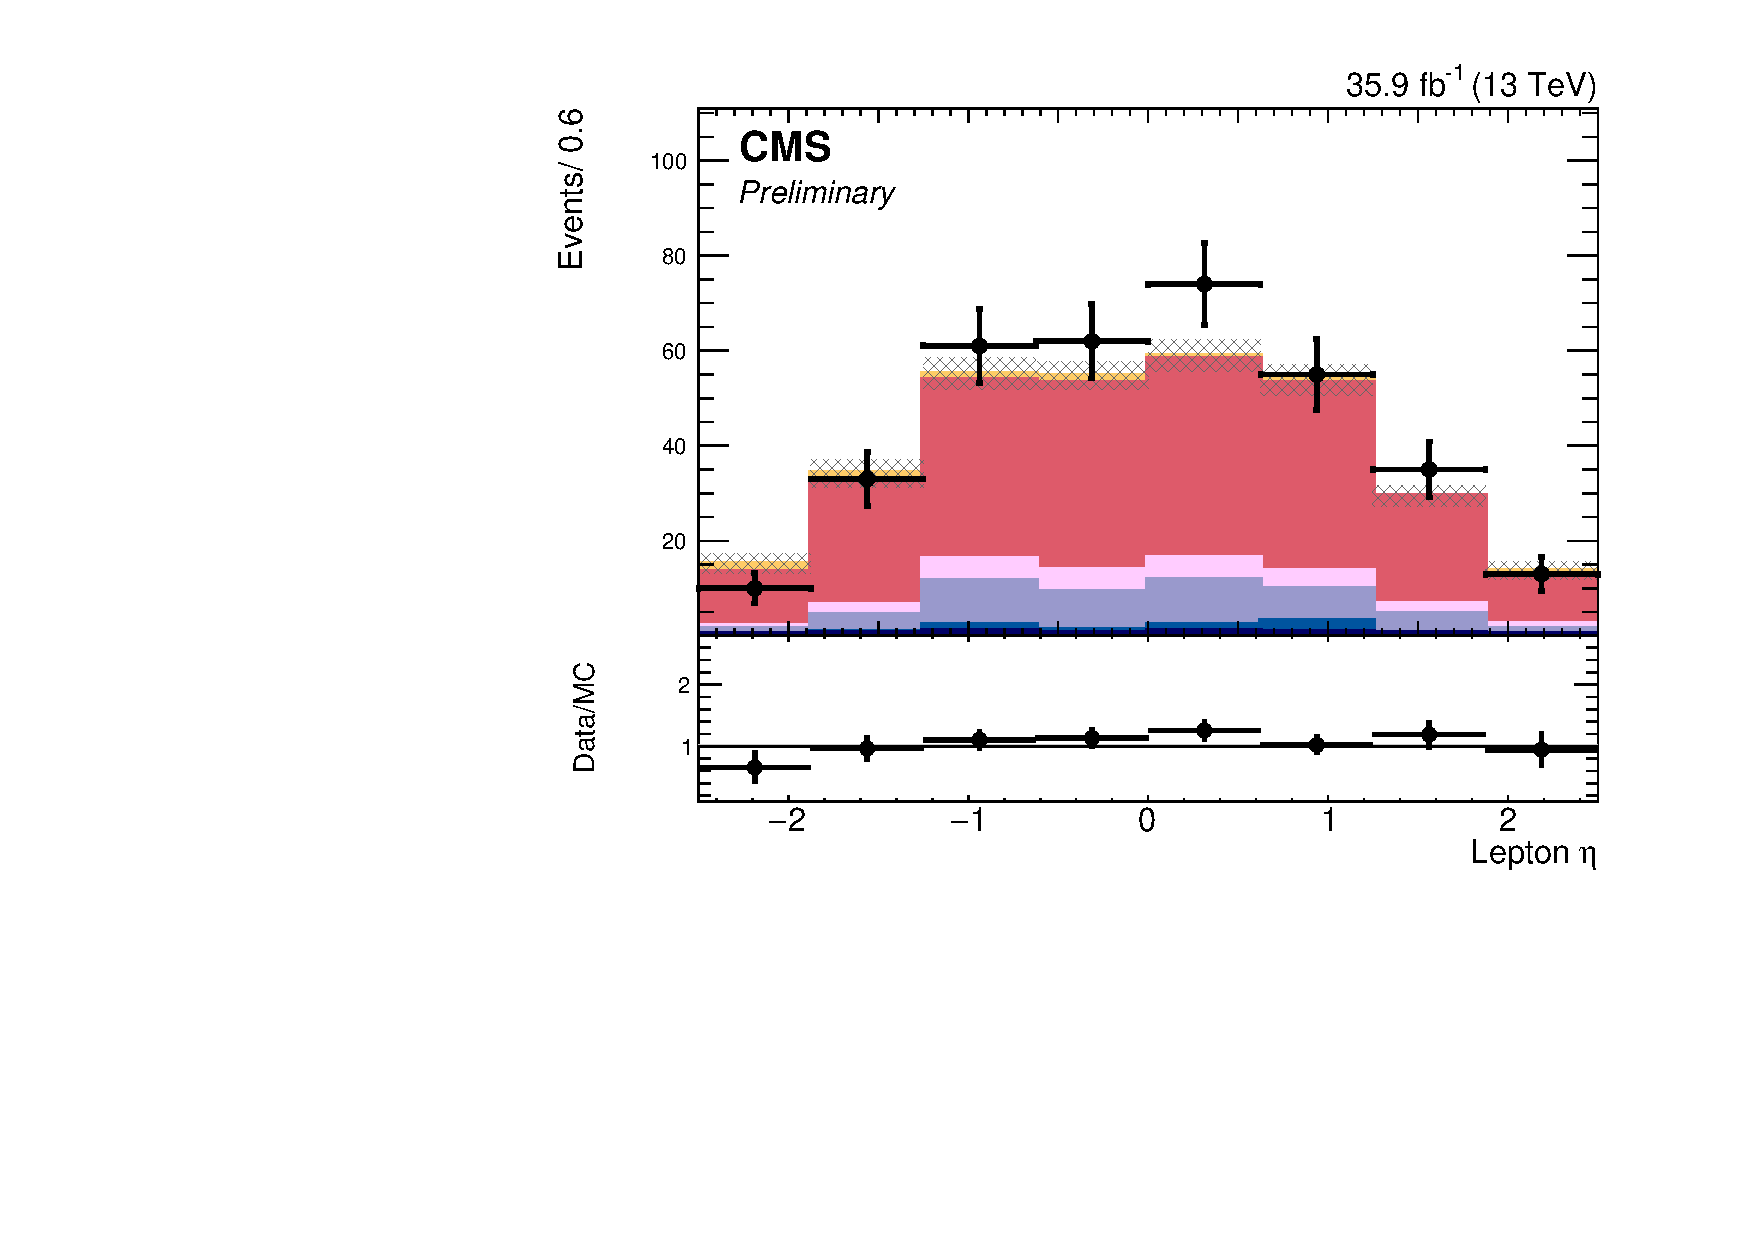
\includegraphics[width=0.45\textwidth]{Plots/plots/DibosonBoostedElMuCuts13TeV_WjetControlRegion_Tighter_CHS_lepton_eta.pdf}
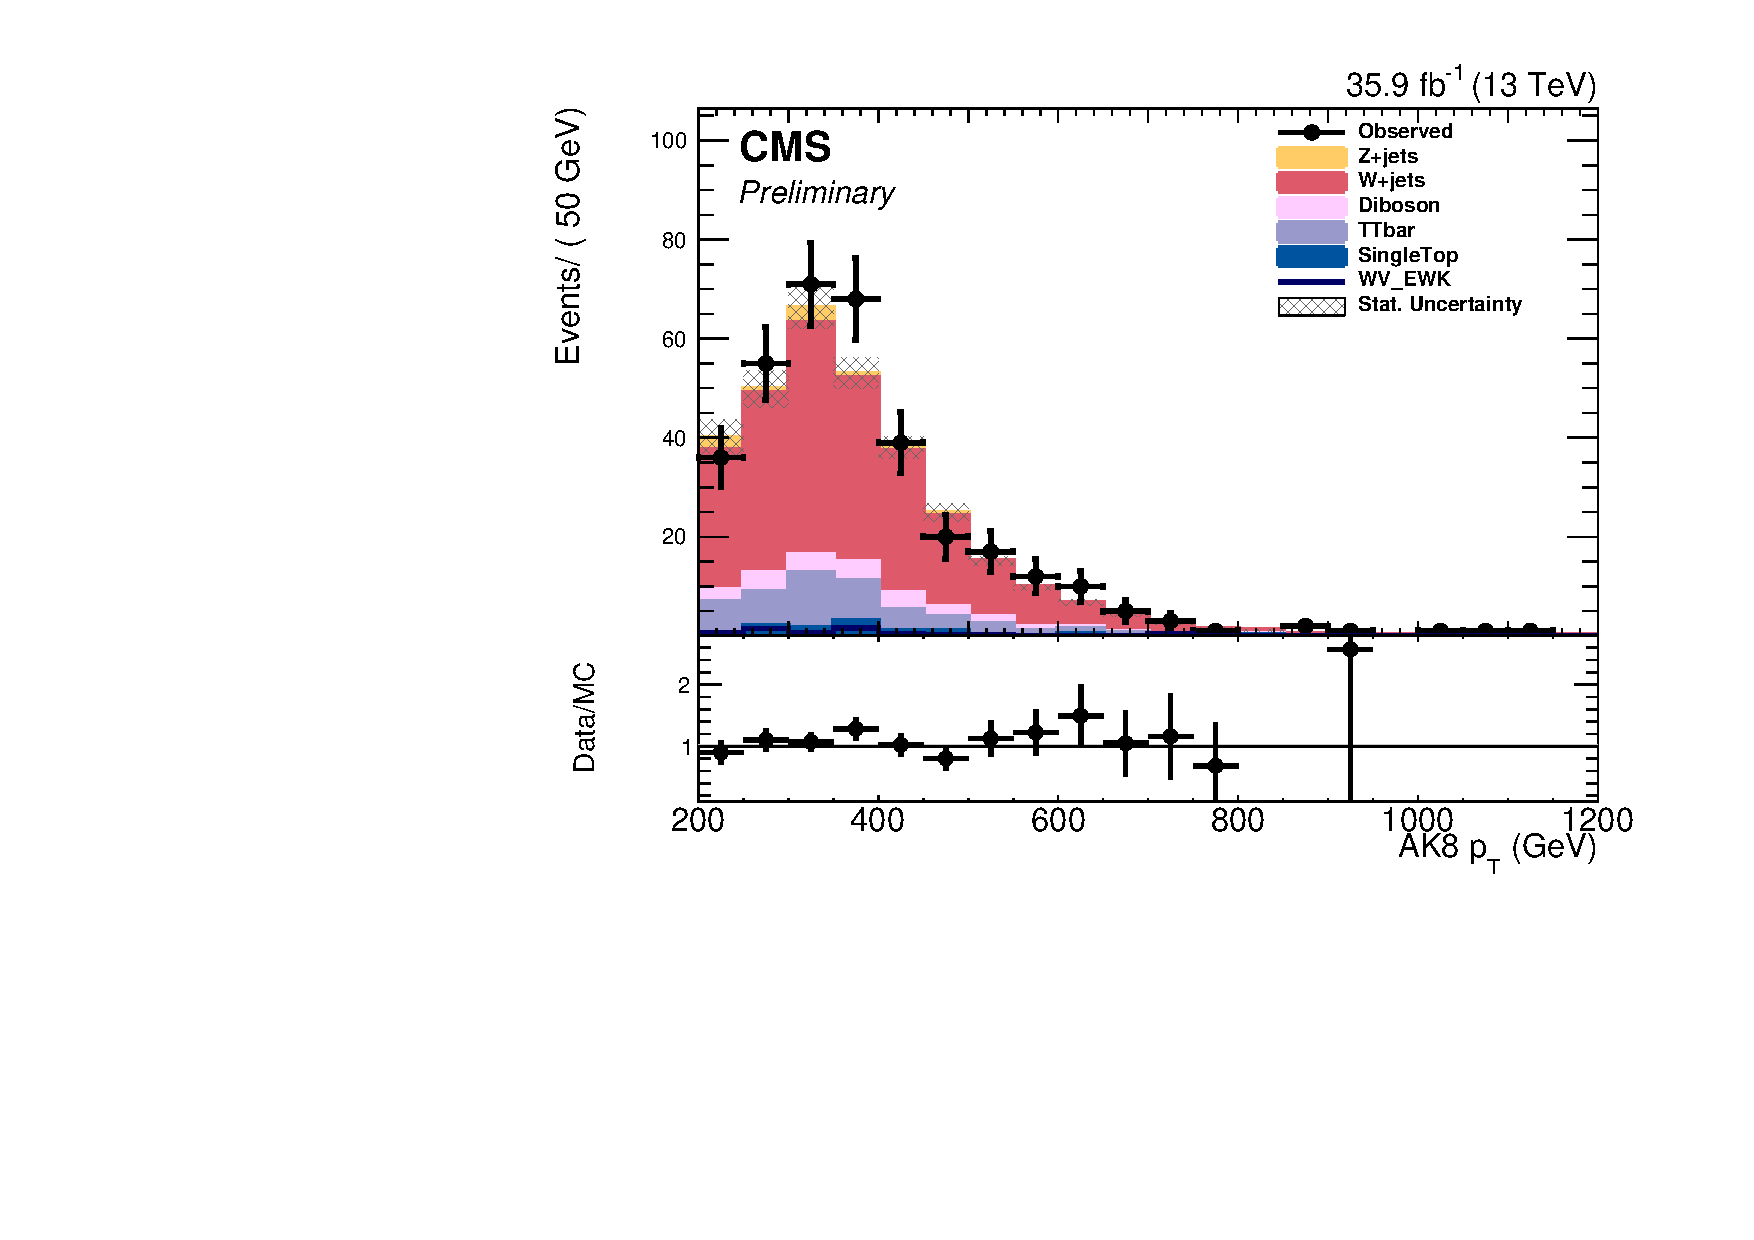
\includegraphics[width=0.45\textwidth]{Plots/plots/DibosonBoostedElMuCuts13TeV_WjetControlRegion_Tighter_CHS_ungroomed_PuppiAK8_jet_pt.pdf}
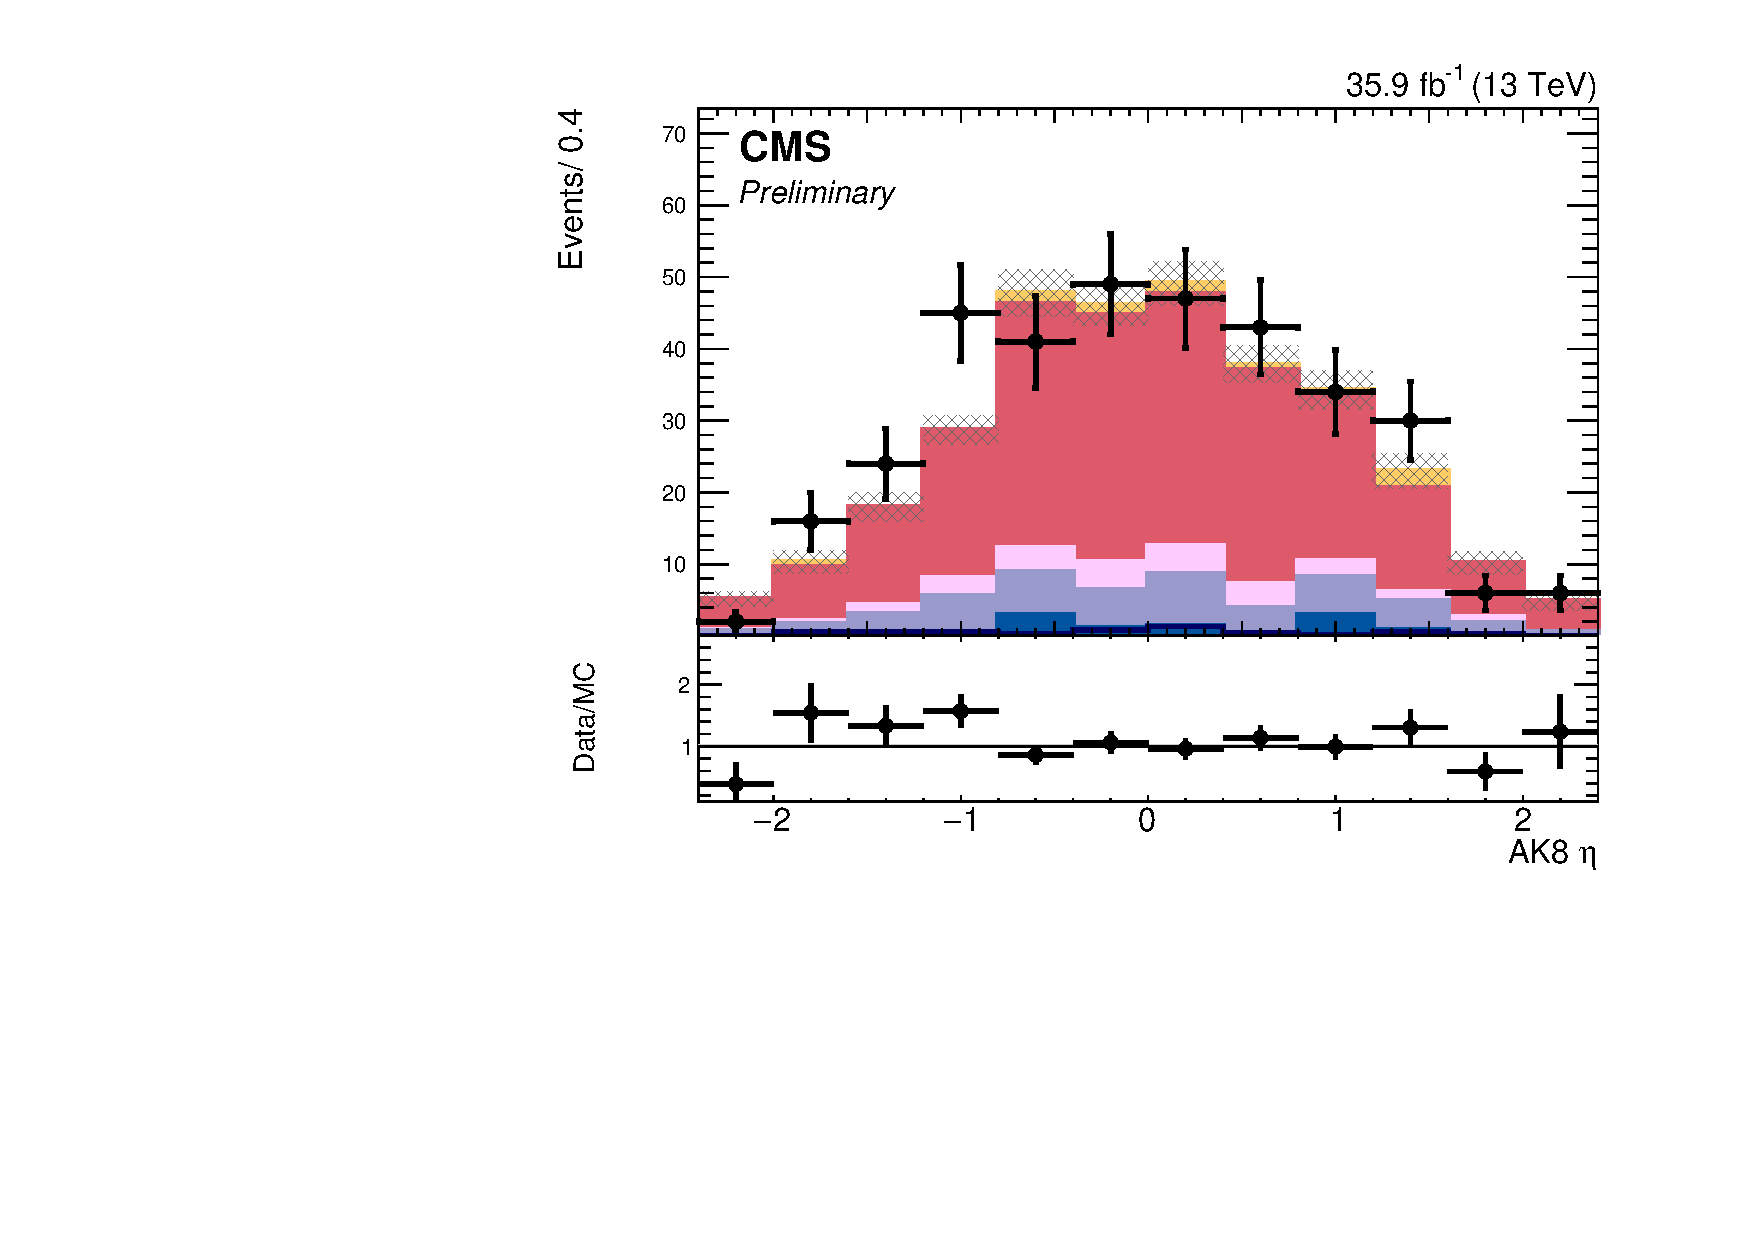
\includegraphics[width=0.45\textwidth]{Plots/plots/DibosonBoostedElMuCuts13TeV_WjetControlRegion_Tighter_CHS_ungroomed_PuppiAK8_jet_eta.pdf}
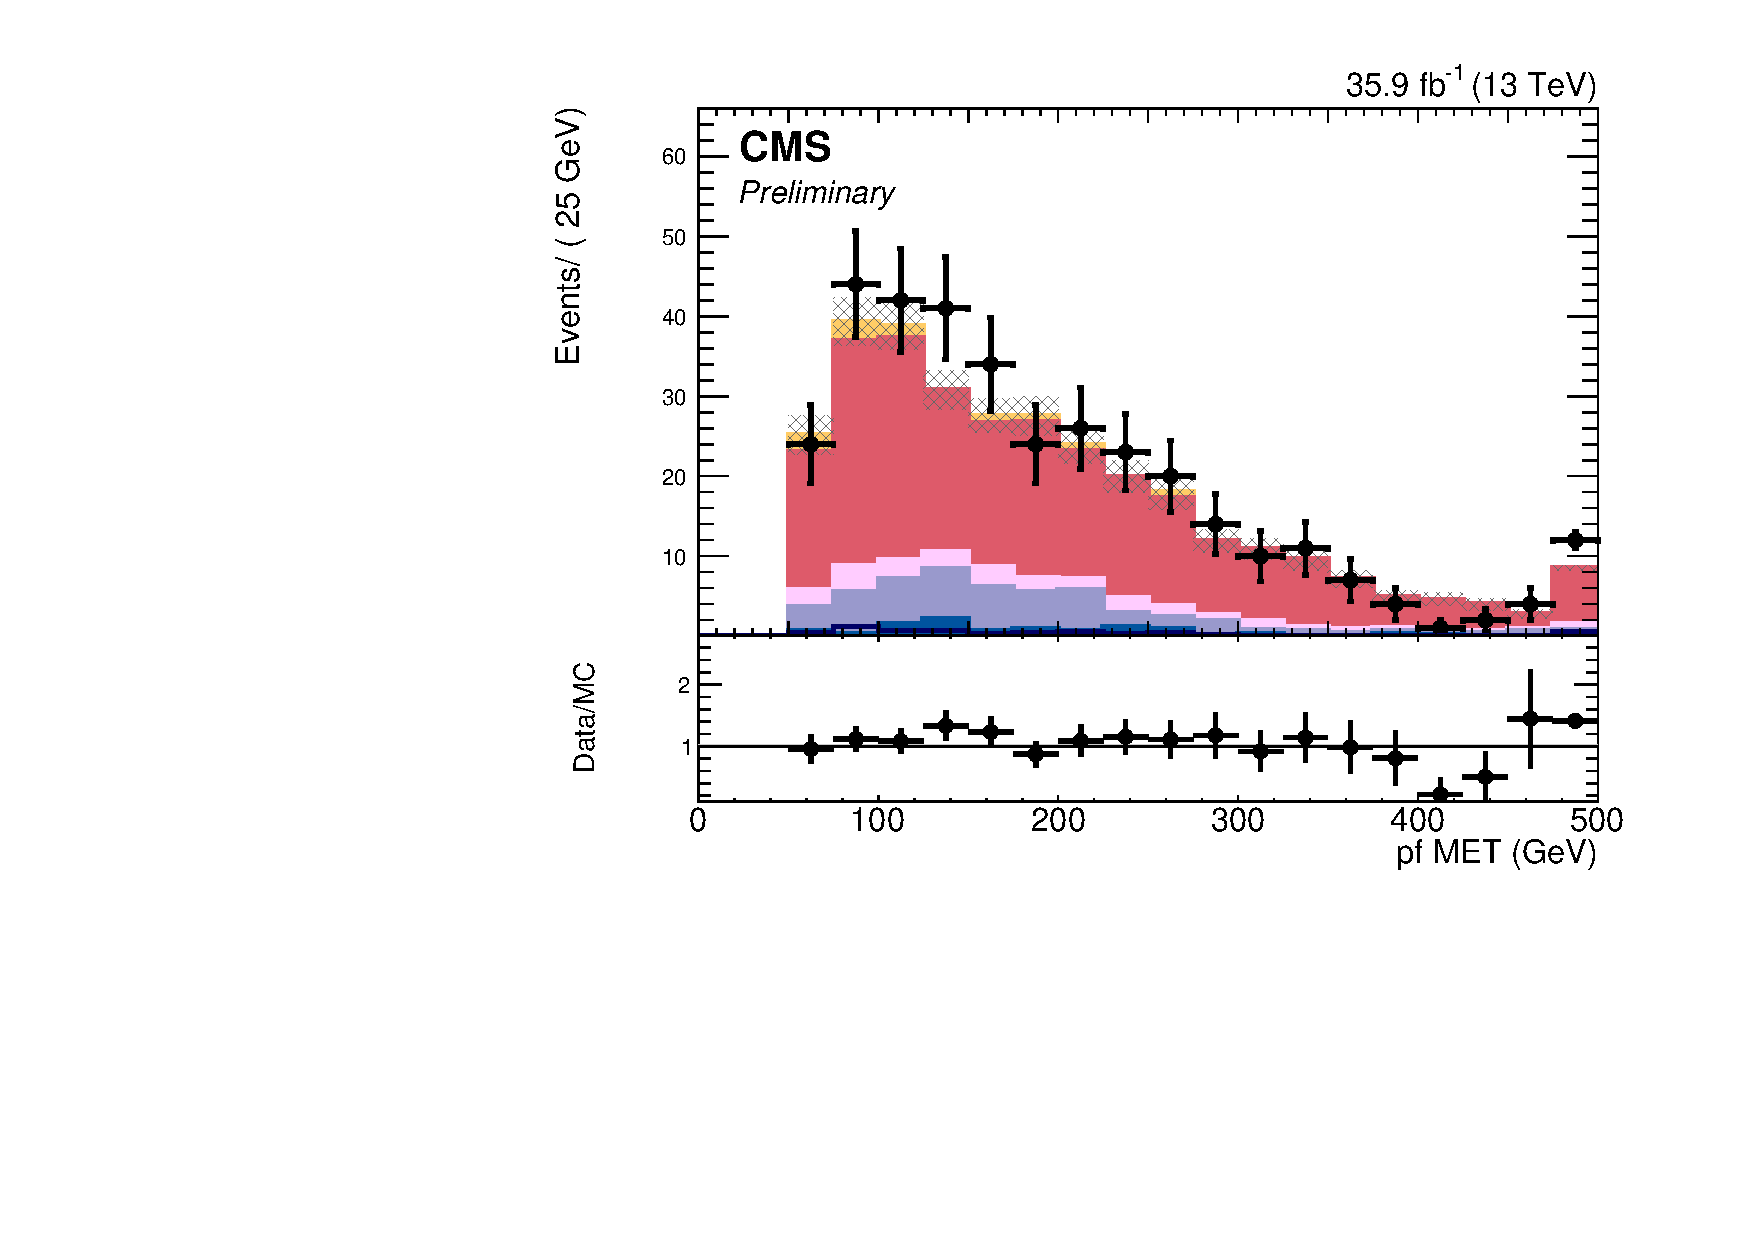
\includegraphics[width=0.45\textwidth]{Plots/plots/DibosonBoostedElMuCuts13TeV_WjetControlRegion_Tighter_CHS_pfMET_Corr.pdf}
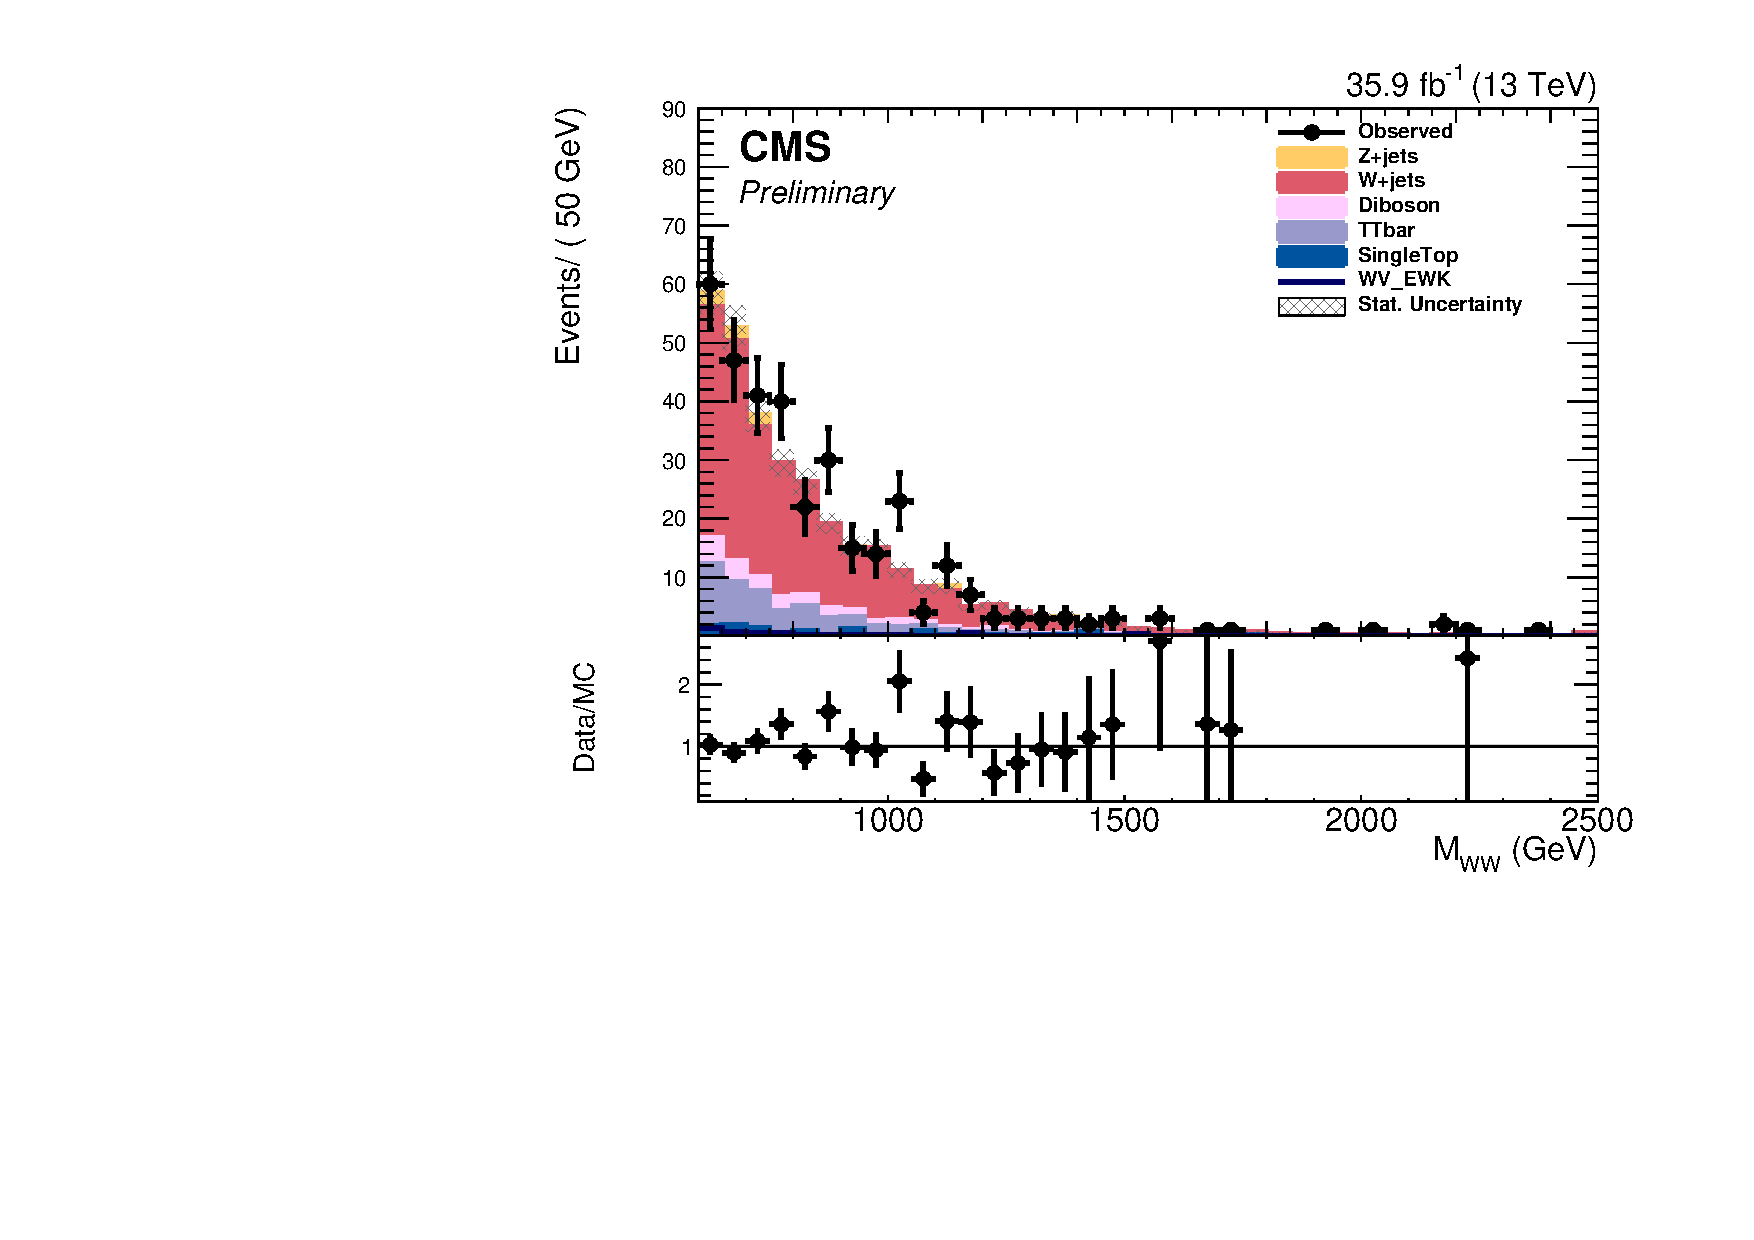
\includegraphics[width=0.45\textwidth]{Plots/plots/DibosonBoostedElMuCuts13TeV_WjetControlRegion_Tighter_CHS_mass_lvj_type0_PuppiAK8.pdf}
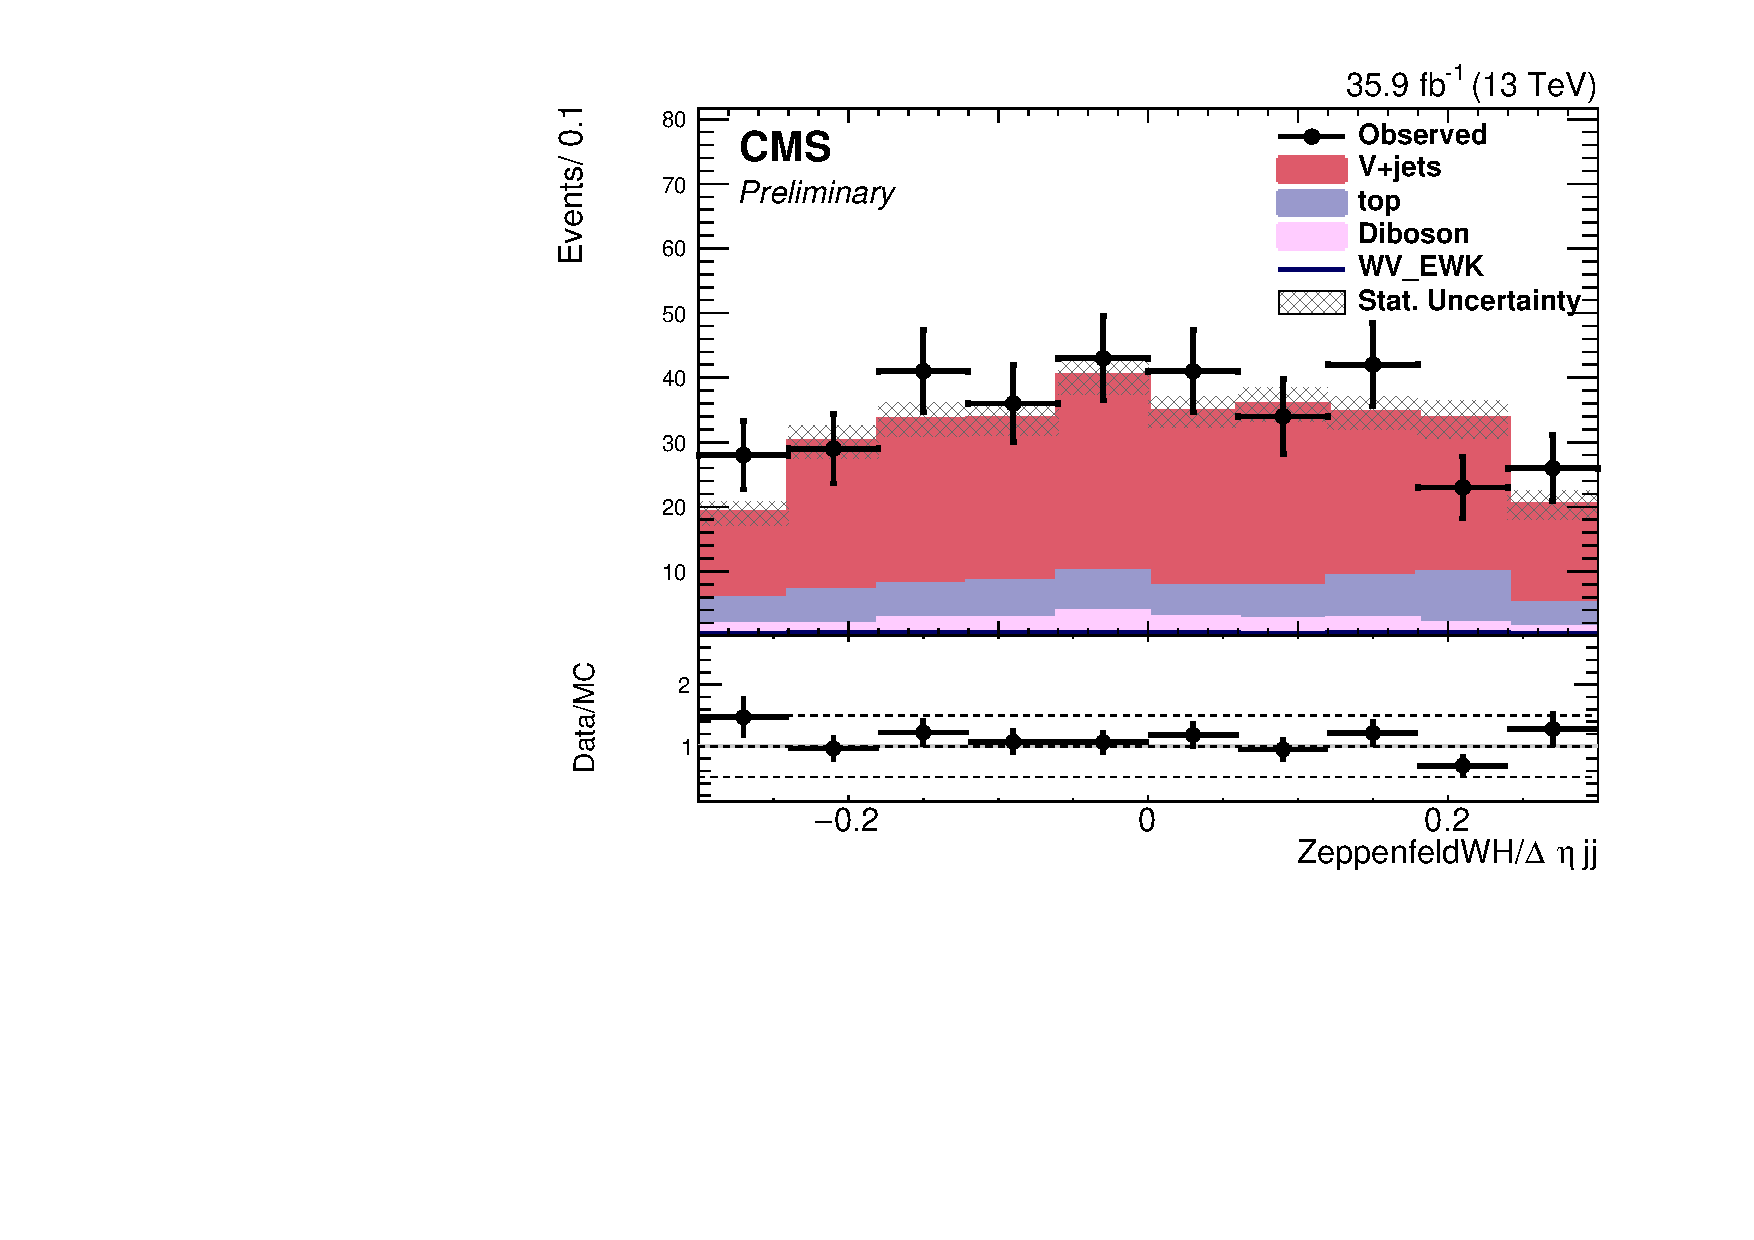
\includegraphics[width=0.45\textwidth]{Plots/plots/DibosonBoostedElMuCuts13TeV_WjetControlRegion_Tighter_CHS_ZeppenfeldWH_new.pdf}
% 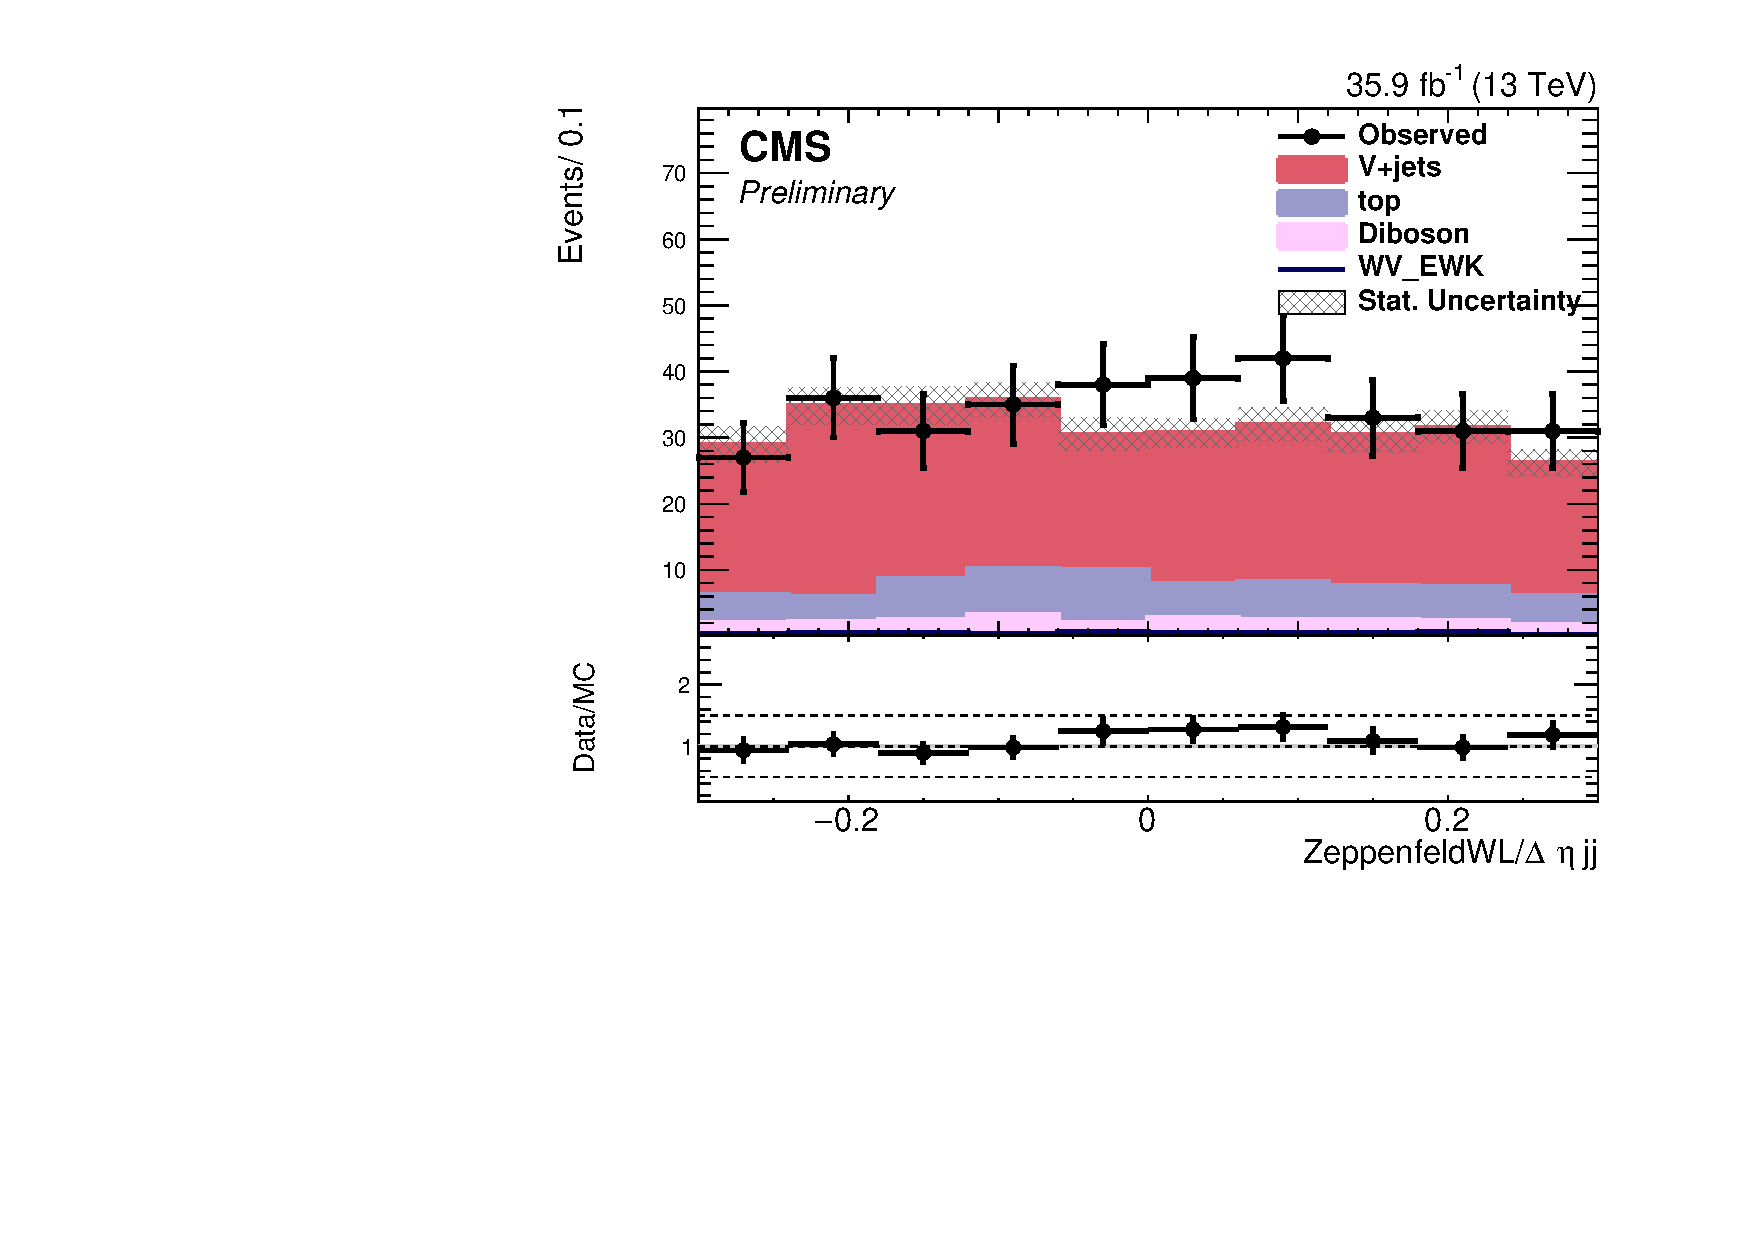
\includegraphics[width=0.45\textwidth]{Plots/plots/DibosonBoostedElMuCuts13TeV_WjetControlRegion_Tighter_CHS_ZeppenfeldWL_type0_new.pdf}
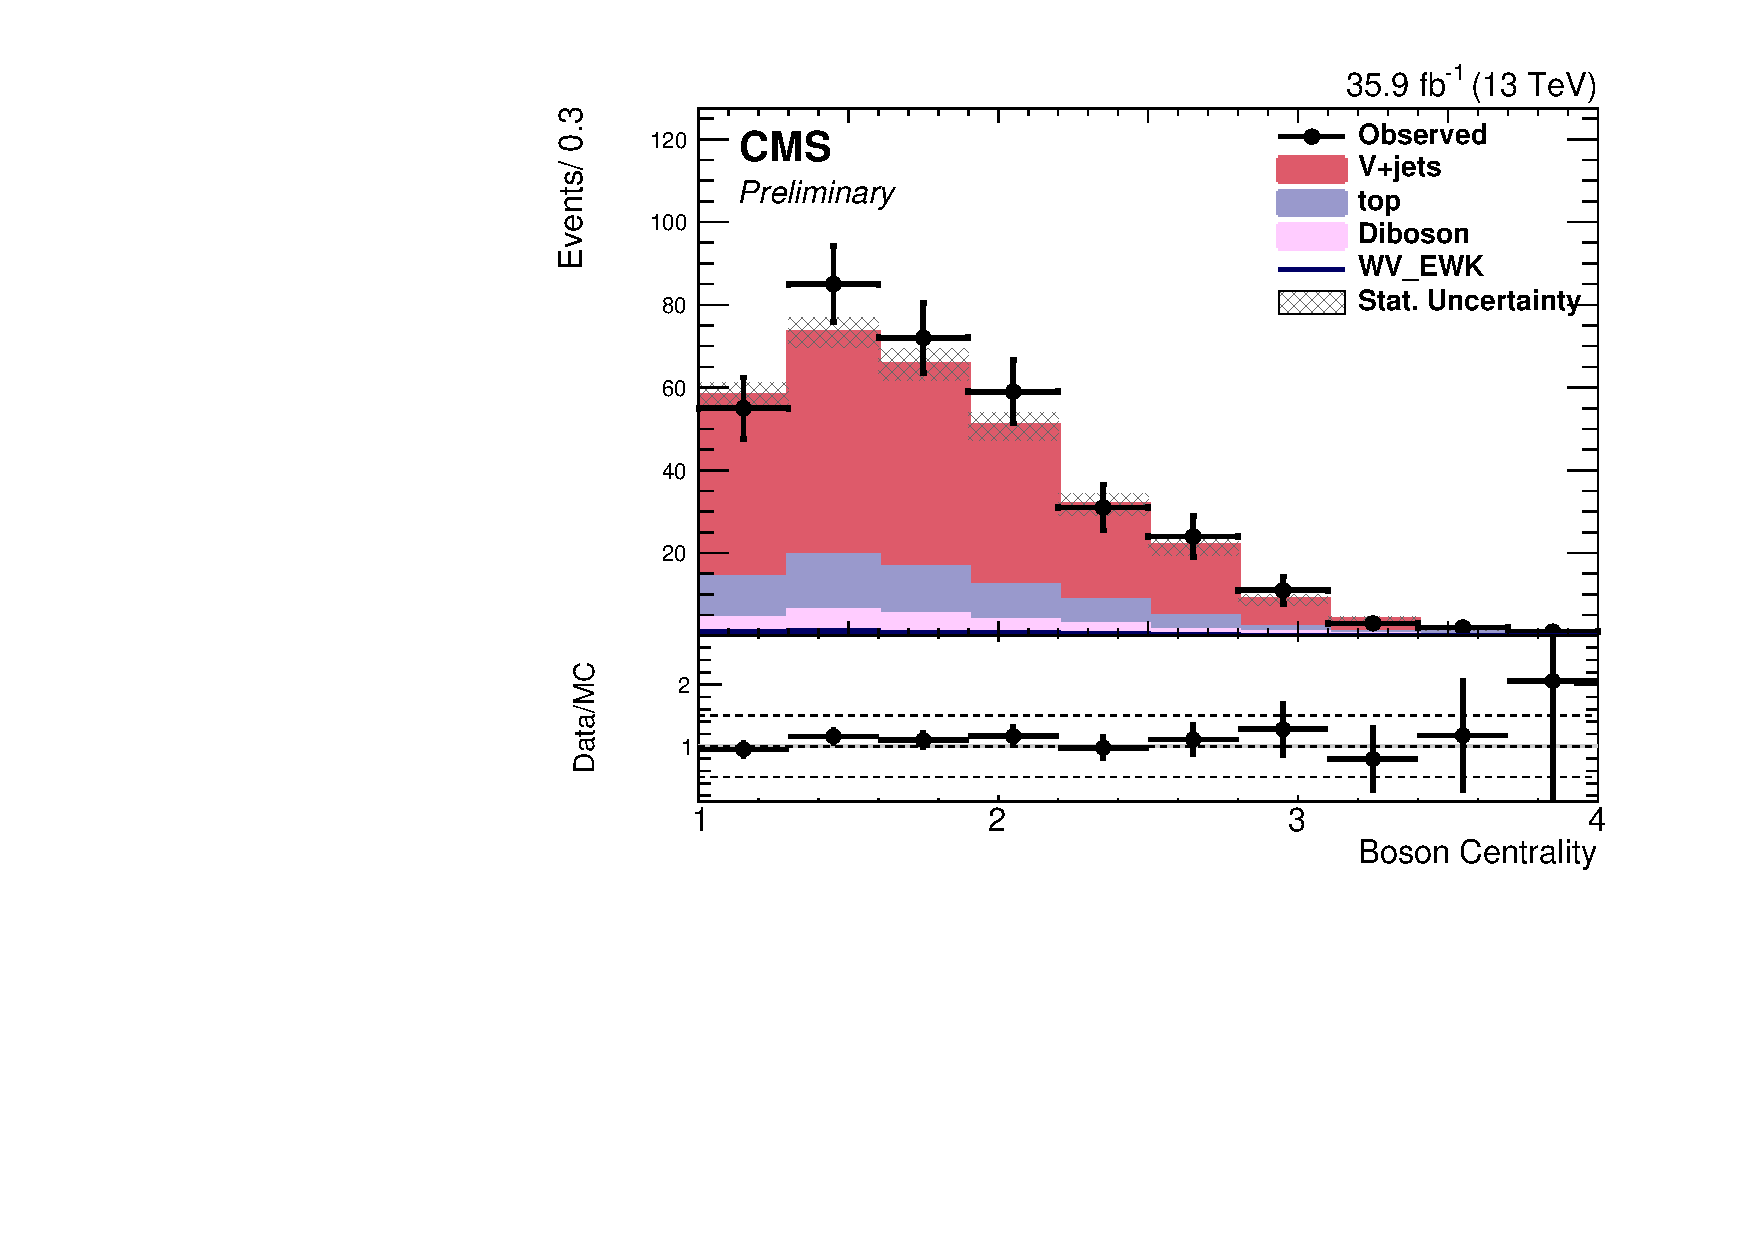
\includegraphics[width=0.45\textwidth]{Plots/plots/DibosonBoostedElMuCuts13TeV_WjetControlRegion_Tighter_CHS_BosonCentrality_type0.pdf}
\caption{Kinematic distributions in the $\PW+$jets background sideband region. $\PW+$jets predictions are taken from the simulation. The hatched bands include statistical uncertainties from the predicted yields.}
\label{fig:wjet_control2}
\end{figure*}

The background estimation described below closely follows the method used in previous inclusive searches in $\PW V$ final state~\cite{VV_resonance_2016,WVaTGC2016}. More detailed description of the method can be found in the references. The shape and normalization of the $\PW+$jets background prediction are estimated from data in the sideband region defined above. The aQGC and charged Higgs limits are extracted from a fit (using the CMS Higgs combination tools) to the $m_{WV}$ distribution in the $\PW V$ final state as shown in Figure~\ref{fig:signal2}. The prediction of the $\PW+$jets background used in the signal extraction is obtained by performing a separate fit to the $m_{WV}$ distribution in the sideband region. The extrapolation factors (denoted as alpha-ratio values) to the signal region are obtained from the $\PW+$jets simulation as a function of the $m_{WV}$ variable as described below. The shapes of the $t\bar{t}$, single top, diboson, and $\PW+$jets processes are represented by parametric shapes extracted from simulation. The following parametric functions are used: 

\begin{description}
	\item [Main function] $f_{ExpTail} = \exp(\frac{-x}{a+bx})$
	\item [Alternate Function] $f_{Exp} = \exp(cx)$
\end{description}

The fits to the corresponding MC predictions are shown in Figure~\ref{fig:mWW_1}. The shown error band is determined by evaluating the fitted functions many times for several points along the x axis with the fitted parameters randomized according to their resulting uncertainties. The extracted fit parameters are summarized in Table~\ref{Table:BackgroundEstimation_mWWFitPars}. These parametric templates are then used to fit the $m_{WV}$ distribution in the sideband region. The normalization and shape of the  $\PW$+jets process is floated in this fit. The other background processes are fixed to the SM predictions. The resulting fit is shown in Figure~\ref{fig:DataMCForMWW}.

\begin{figure}[!htbp] 
	 \centering 
	 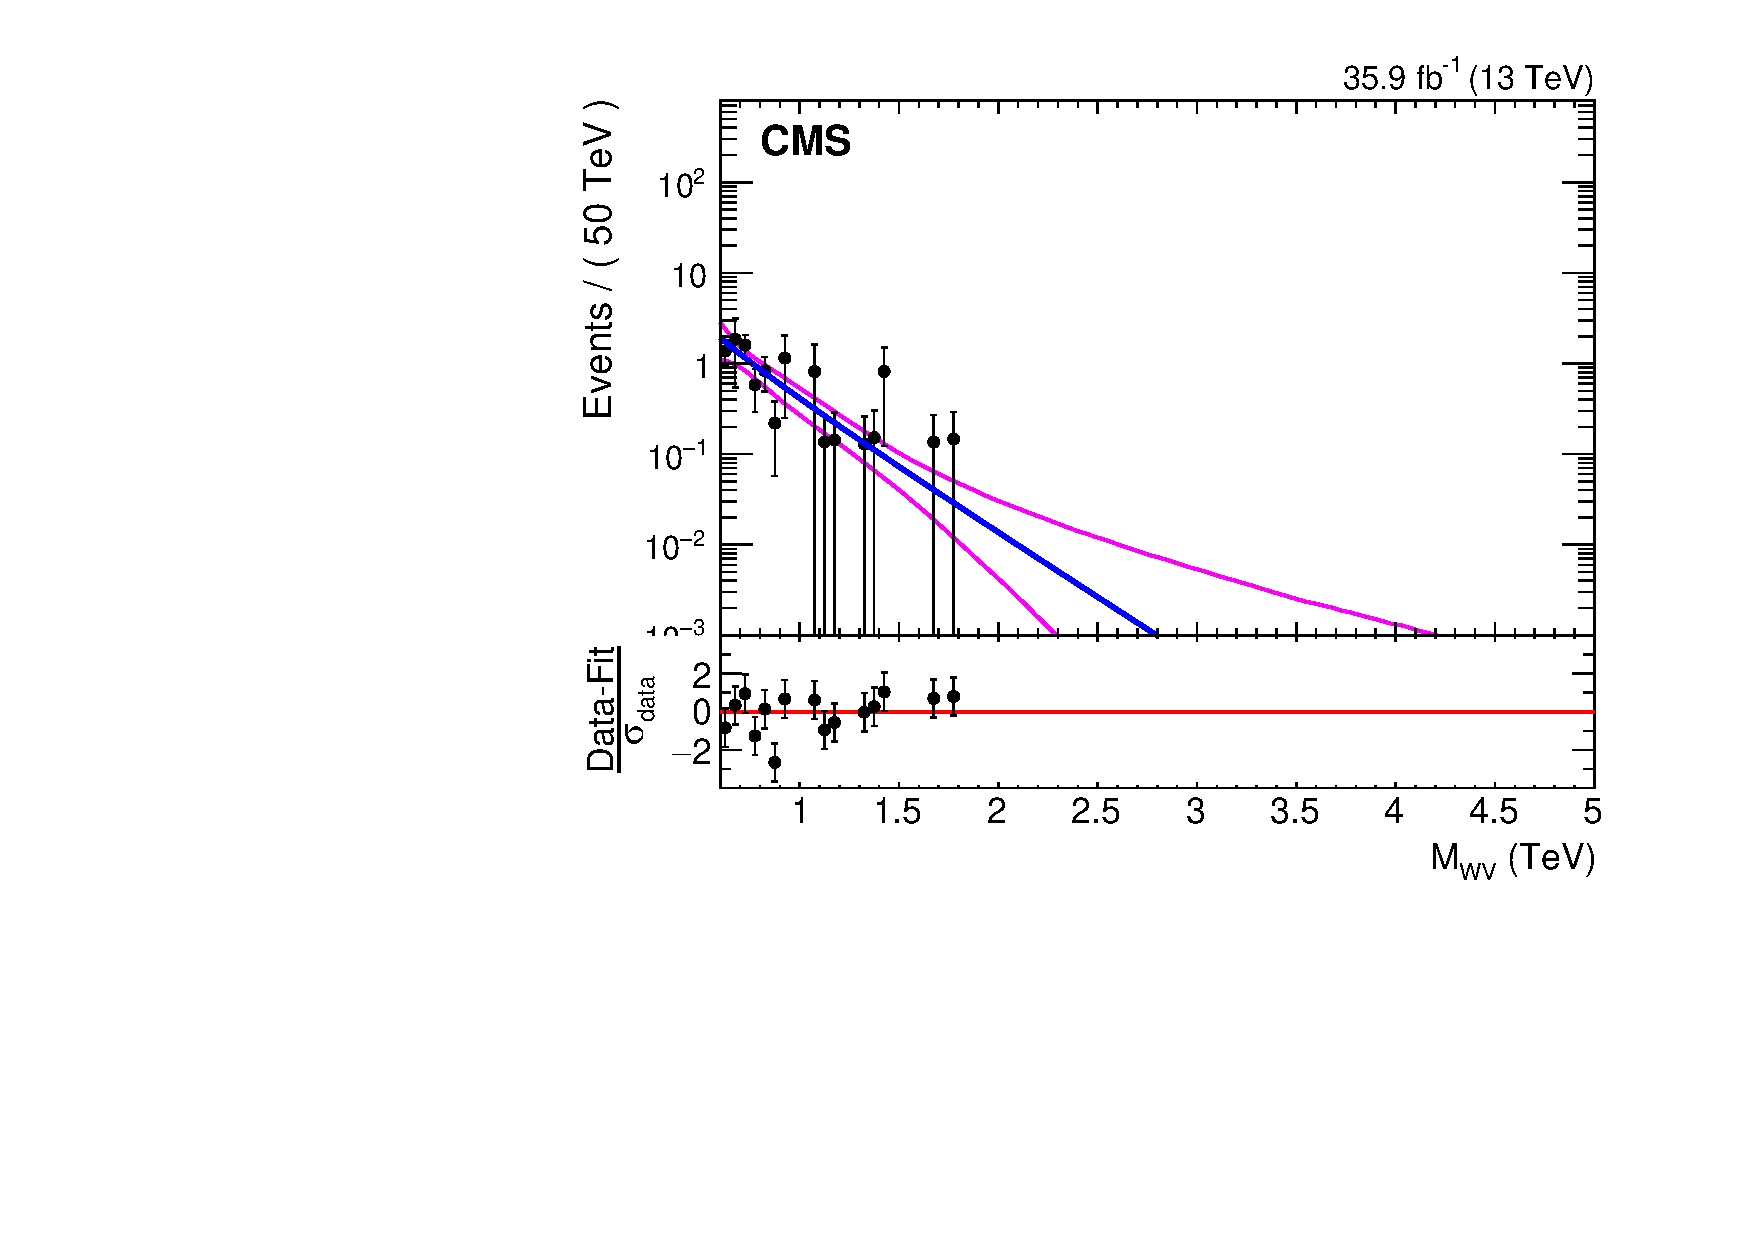
\includegraphics[width=0.45\textwidth]{Plots/BackgroundEstimation/WV/m_lvj_fitting/WWTree_STop_m_lvj_sb_loExpN_with_pull_log.pdf}
	 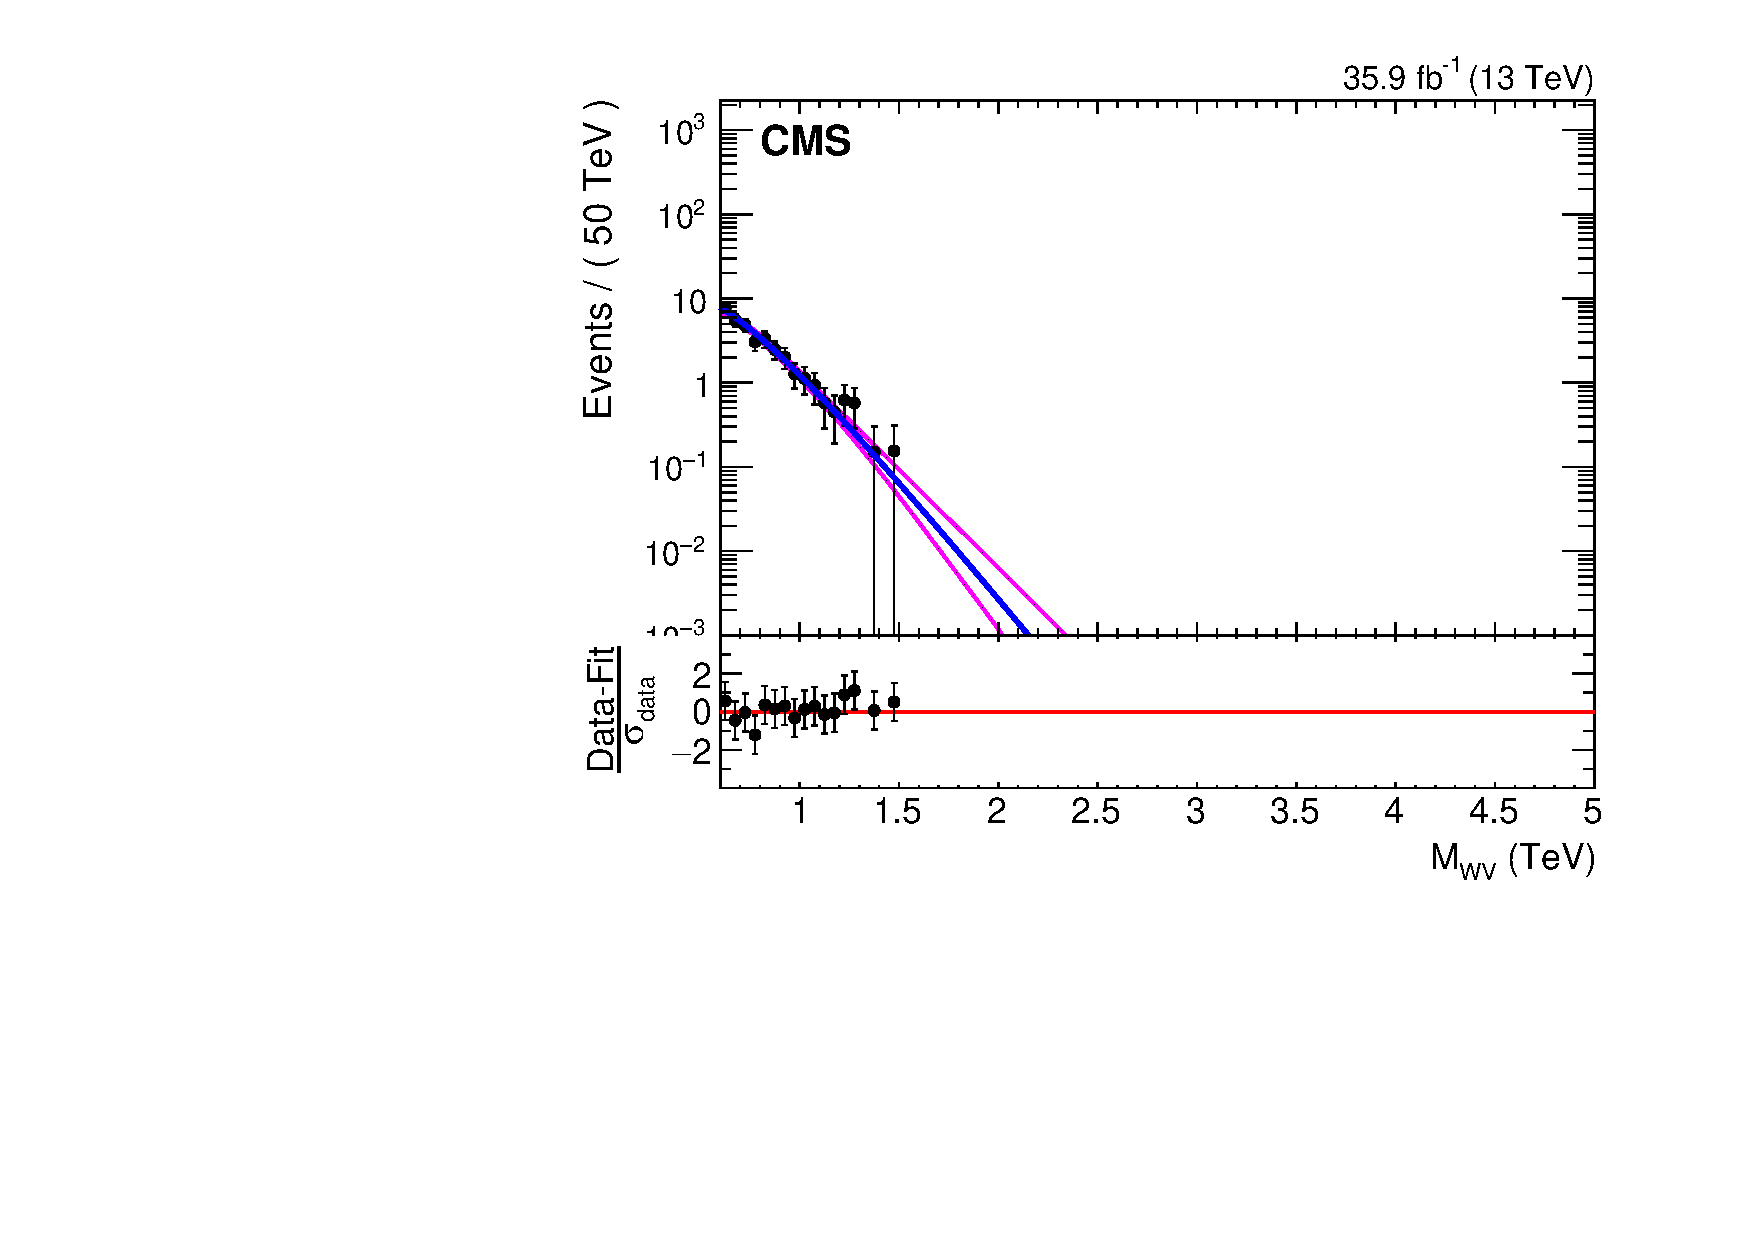
\includegraphics[width=0.45\textwidth]{Plots/BackgroundEstimation/WV/m_lvj_fitting/WWTree_TTbar_m_lvj_sb_loExpN_with_pull_log.pdf}
	 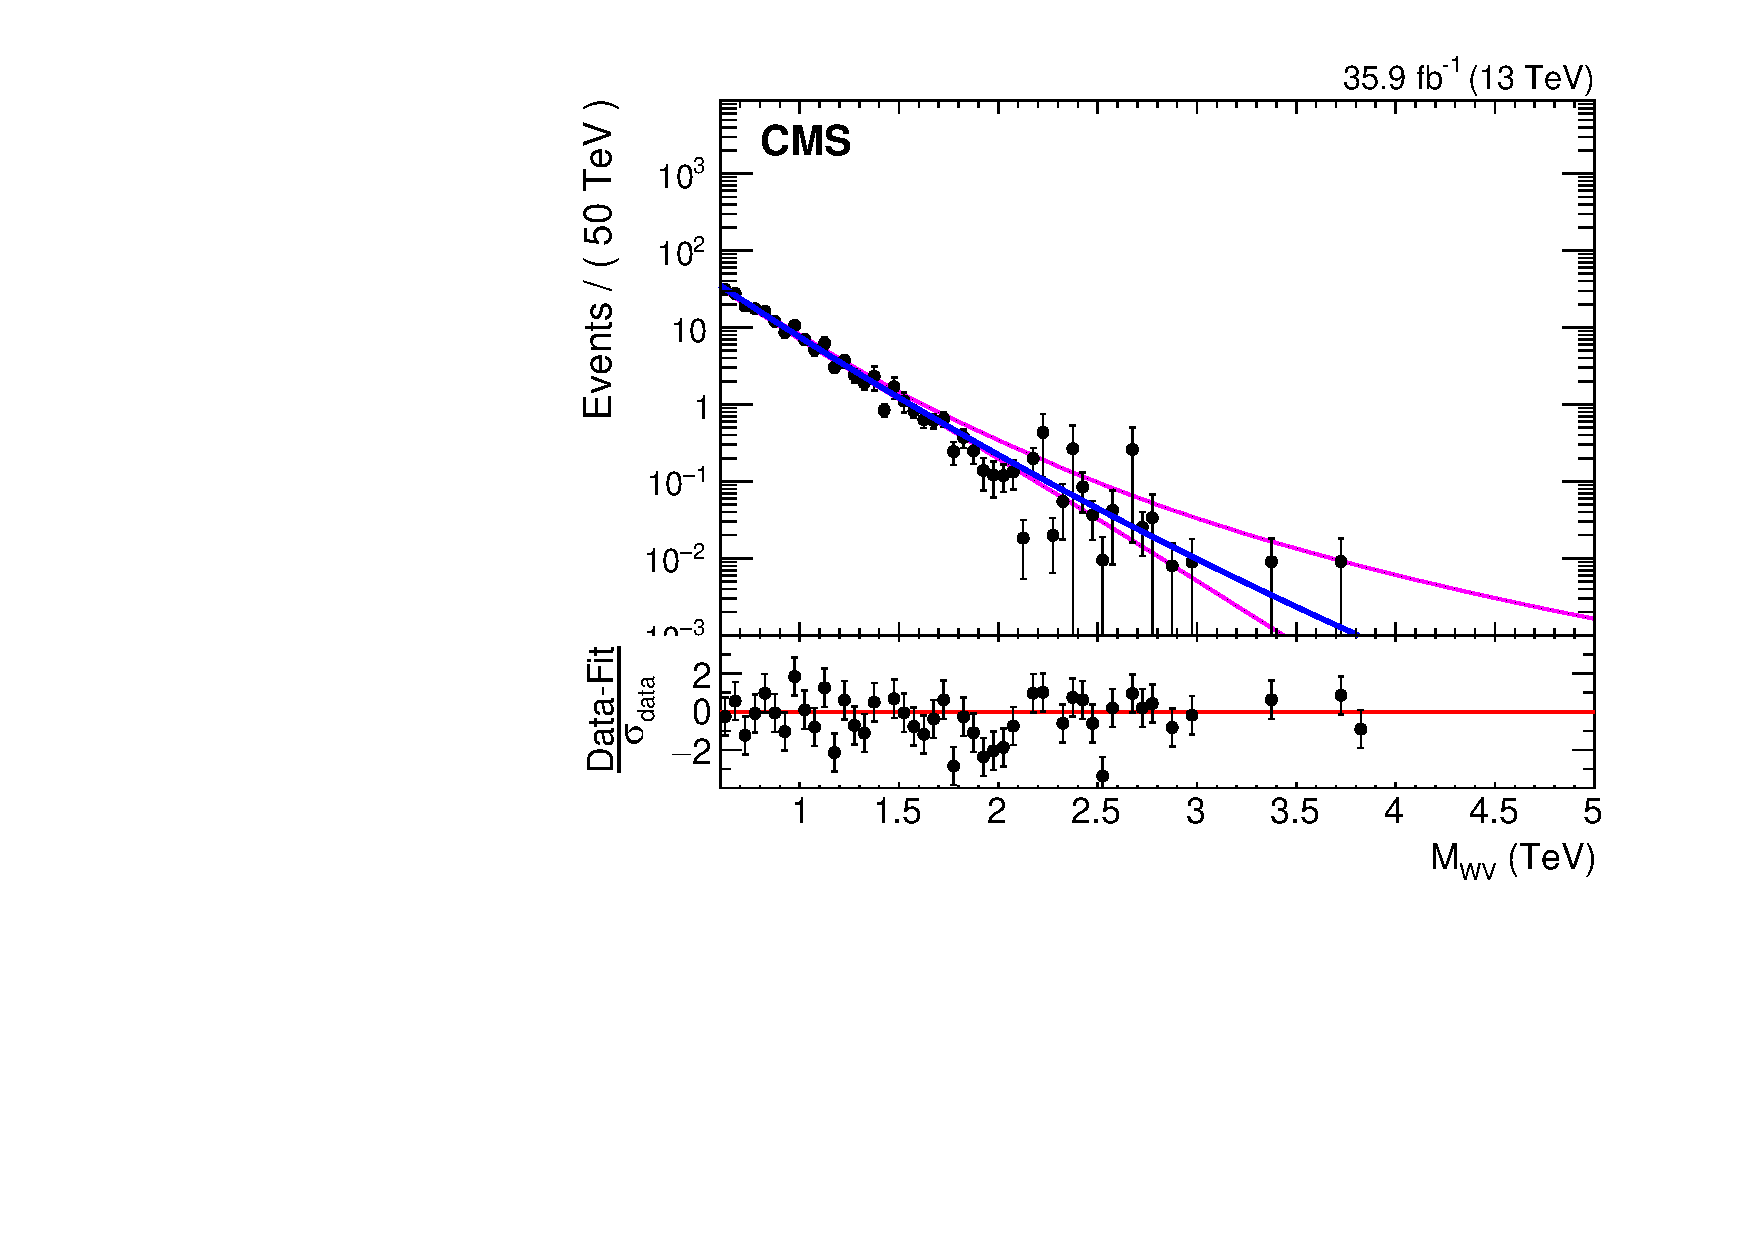
\includegraphics[width=0.45\textwidth]{Plots/BackgroundEstimation/WV/m_lvj_fitting/WWTree_VJets_m_lvj_sb_loExpTail_with_pull_log.pdf}
	 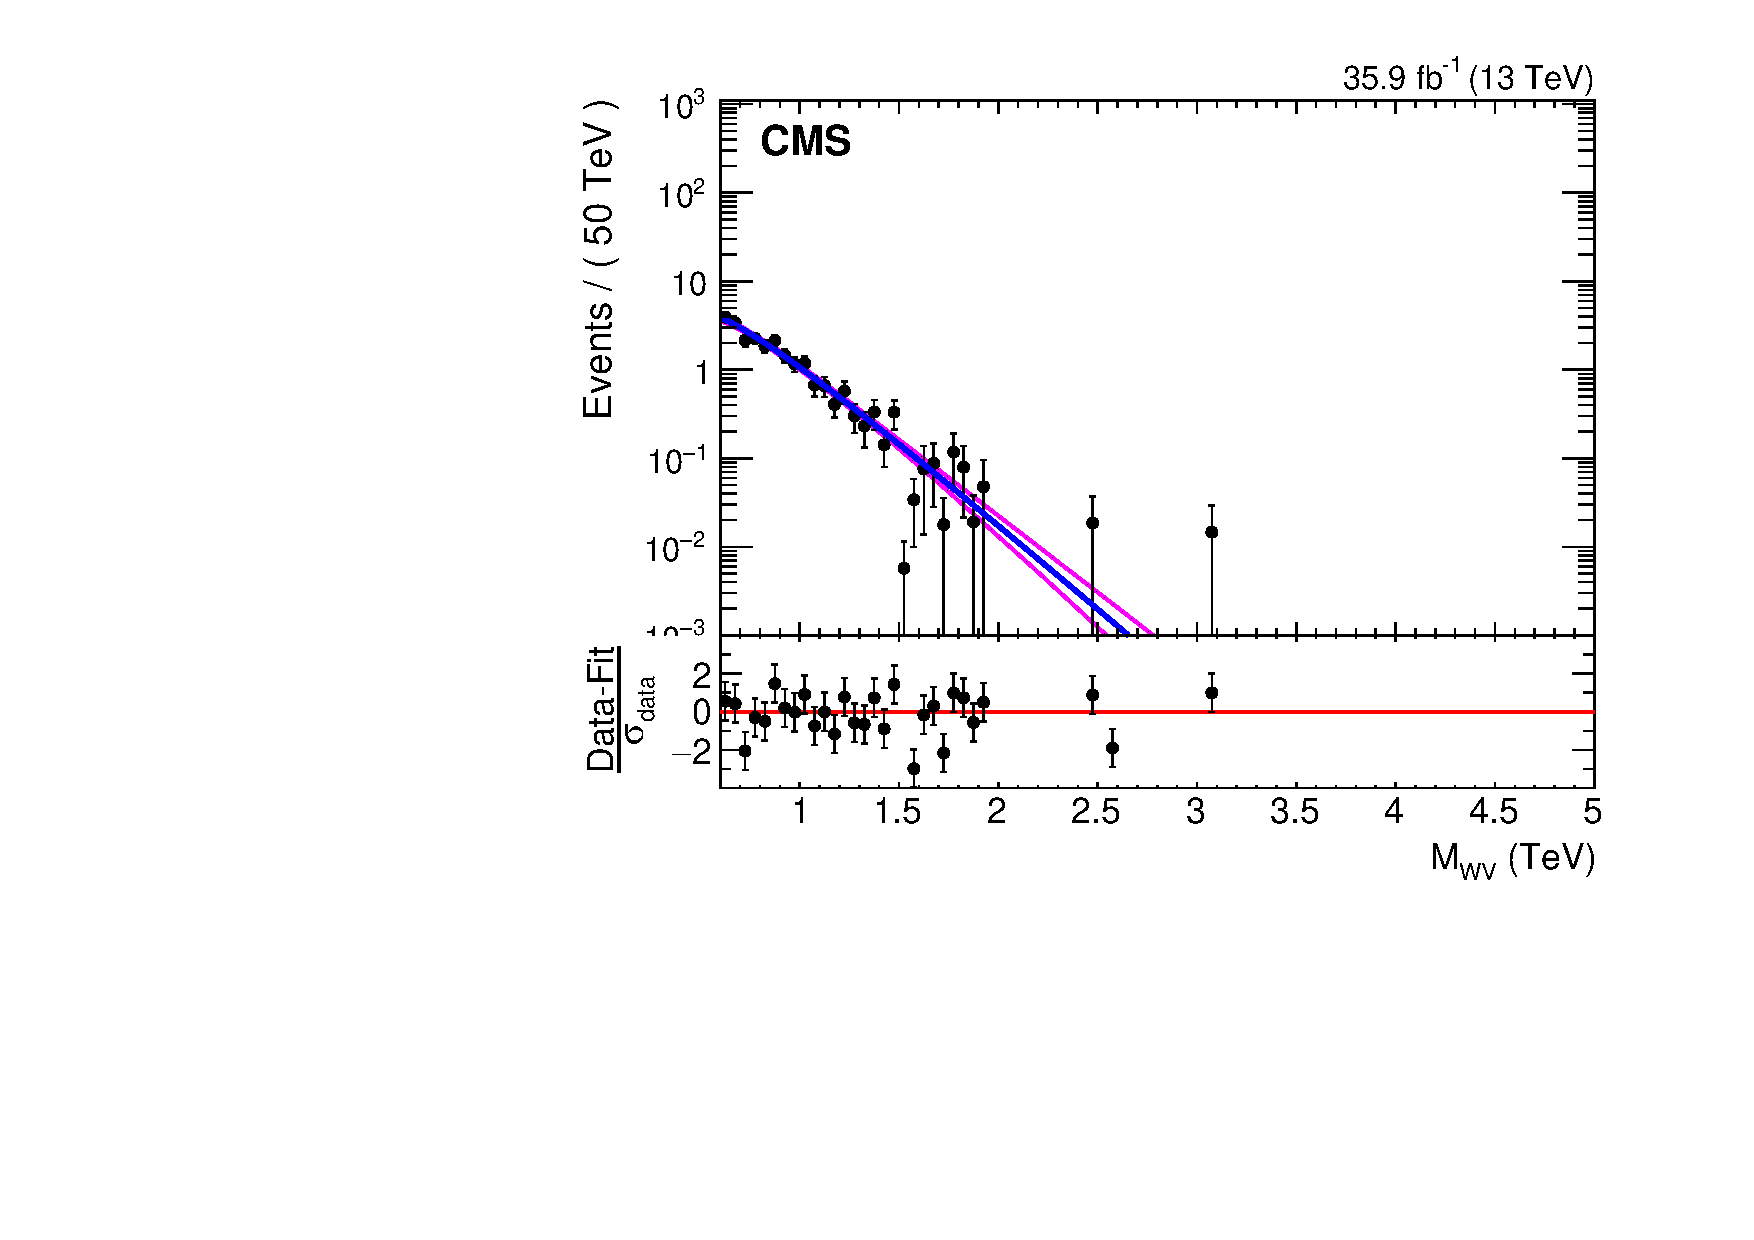
\includegraphics[width=0.45\textwidth]{Plots/BackgroundEstimation/WV/m_lvj_fitting/WWTree_VV_EWK_QCD_m_lvj_sb_loExpN_with_pull_log.pdf}
	 \caption{MC-data and fit shape $m_{WV}$ distributions in the sideband region. From top to bottom: single top, $t\bar{t}$, $\PW+$jets and dibosons.}
	 \label{fig:mWW_1}
\end{figure}





\begin{table}[!htbp]
	\centering
	\begin{tabular}{||c | c||} 
	 \hline
	 parameter & Values \\
	 \hline \hline
	 \multicolumn{2}{|c|}{W+jets, $f_{ExpTail}$}\\
	 \hline
	 a 			&	0.036 $\pm$ 0.026\\
	 b 			&	196.282	$\pm$ 69.671\\
	 $N$ 		&	240.834 $\pm$ 17.917\\
	 \hline \hline
	 \multicolumn{2}{|c|}{W+jets (alternate function), $f_{Exp}$}\\
	 \hline
	 c 			&	-0.003 $\pm$ 0.000\\
	 $N$ 		&	240.690 $\pm$ 17.918\\
	 \hline \hline
	 \multicolumn{2}{|c|}{Diboson, $f_{ExpN}$}\\
	 \hline
	 c 			&	-0.004 $\pm$ 0.001\\
	 n 			&	-203.630 $\pm$ 424.762\\
	 $N$ 		&	27.431 $\pm$ 1.101\\
	 \hline \hline
	 \multicolumn{2}{|c|}{TTbar, $f_{ExpN}$}\\
	 \hline
	 c 			&	-0.007 $\pm$ 0.001\\
	 n 			&	-983.791 $\pm$ 914.875\\
	 $N$ 		&	42.010 $\pm$ 2.512\\
	 \hline \hline
	 \multicolumn{2}{|c|}{Single Top, $f_{ExpN}$}\\
	 \hline
	 c 			&	-0.003 $\pm$ 0.002\\
	 n 			&	1045.480 $\pm$ 2235.030\\
	 $N$ 		&	10.511 $\pm$ 2.117\\
	 \hline \hline
	\end{tabular}
 	\caption{Extracted fit parameters for the functions describing the $m_{WV}$ distributions.}
 	\label{Table:BackgroundEstimation_mWWFitPars}
\end{table}


\begin{figure}[!htbp] 
	 \centering 
	 \begin{tabular}{cc}
	 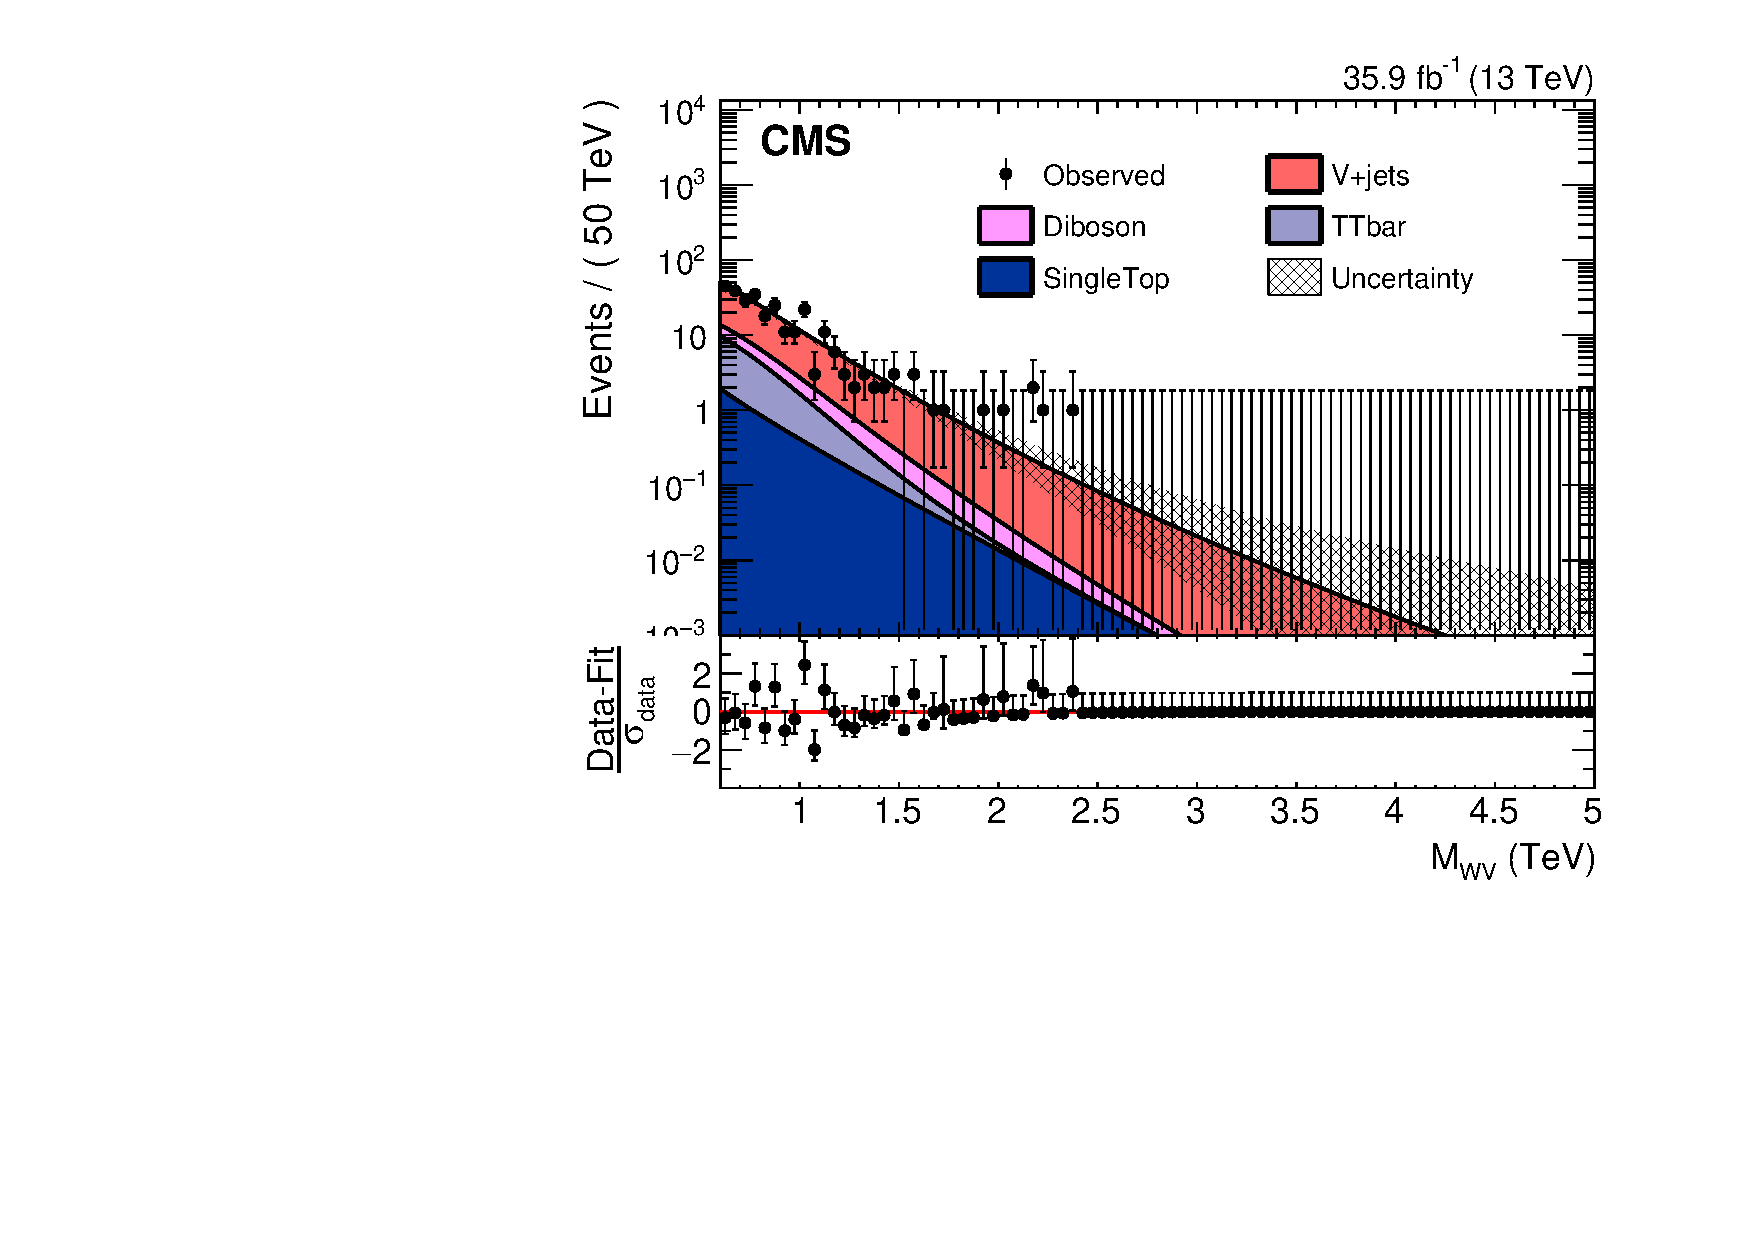
\includegraphics[width=0.48\textwidth]{Plots/BackgroundEstimation/WV/m_lvj_fitting/m_lvj_sb_lo_WJets0_xww__with_pull_log.pdf}
	 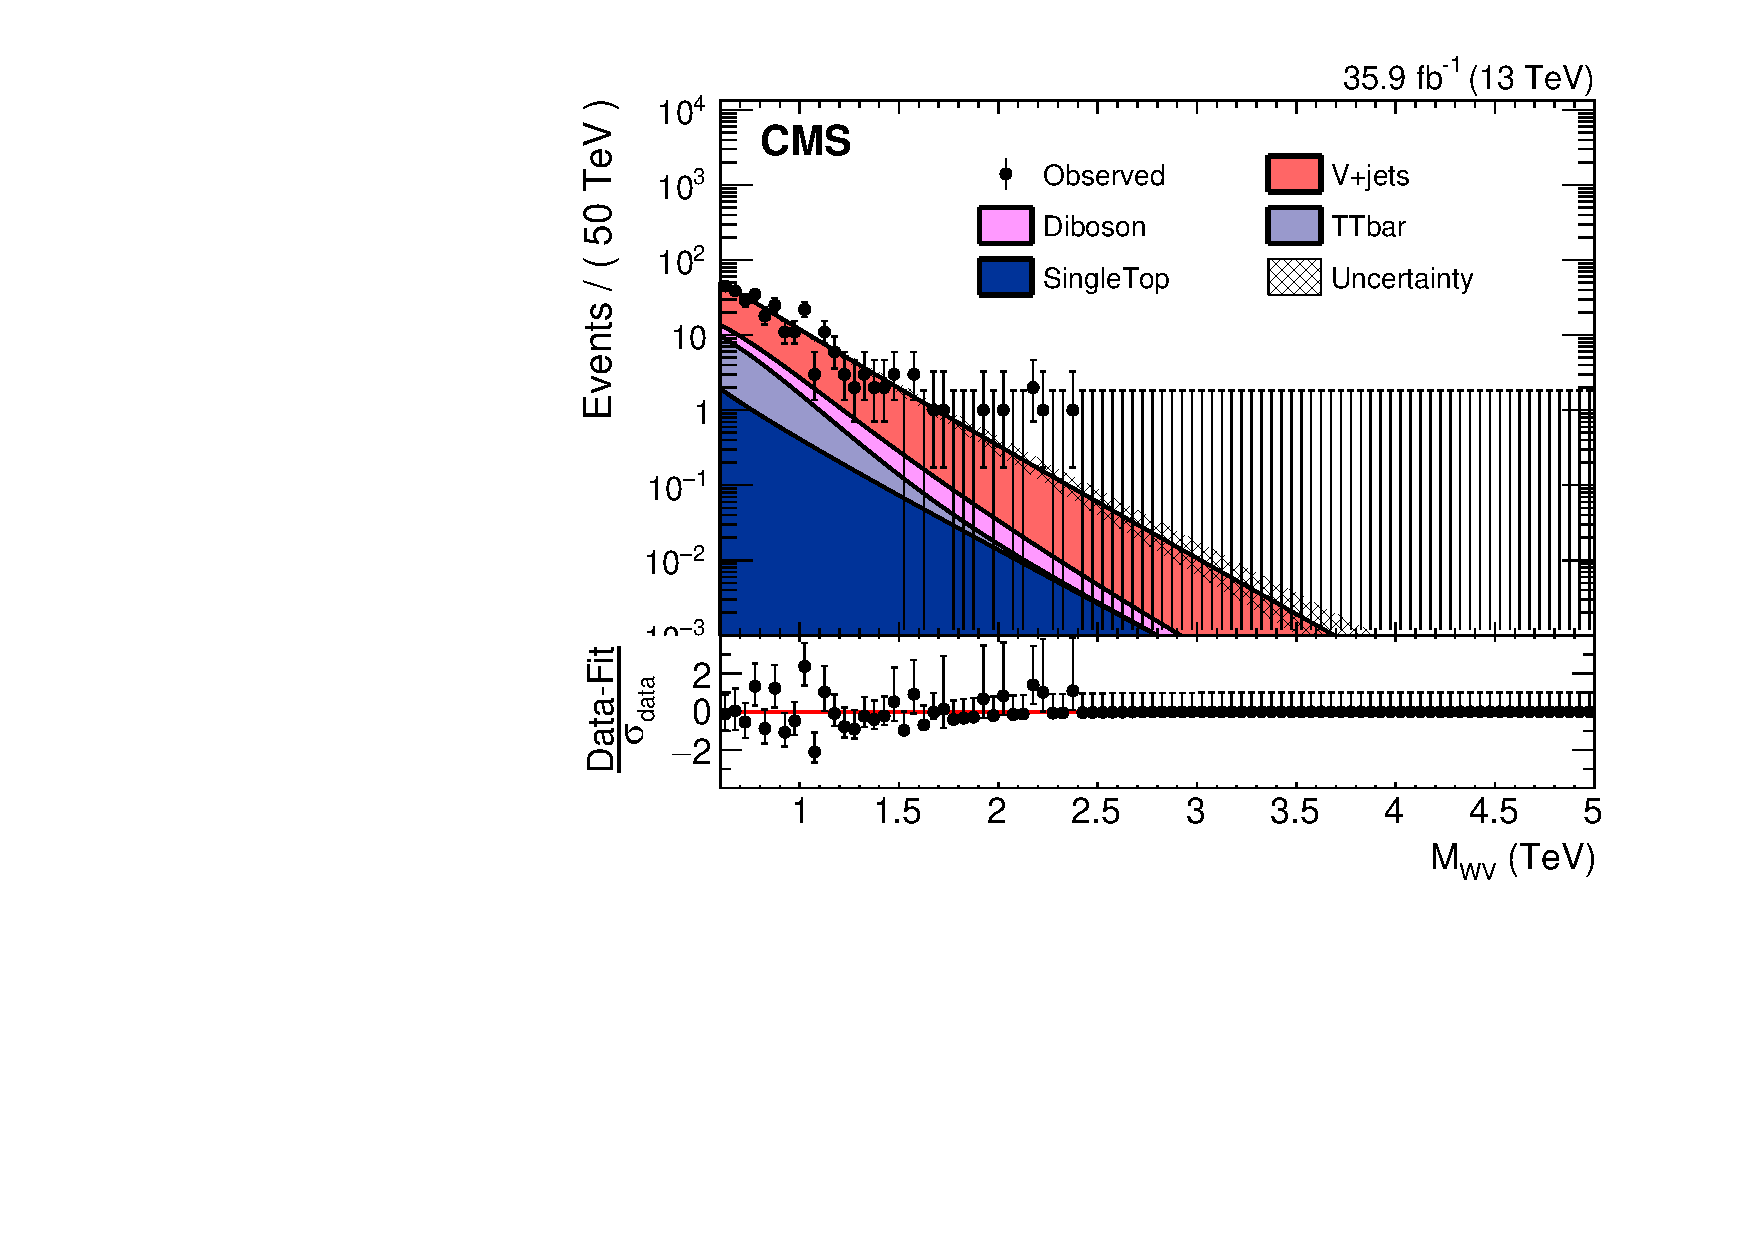
\includegraphics[width=0.48\textwidth]{Plots/BackgroundEstimation/WV/m_lvj_fitting/m_lvj_sb_lo_WJets01_xww__with_pull_log.pdf} 
	 \end{tabular}
	 \caption{The data distribution and the corresponding fit of the $m_{WV}$ distribution in the sideband region for the nominal parametric function (left) and a modified parametric function (right).}
	 \label{fig:DataMCForMWW}
\end{figure}

 The contribution of the $\PW+$jets process in the signal region is obtained using the alpha-ratio-method~\cite{VV_resonance_2016,WVaTGC2016}. The alpha-ratio values extrapolate the $\PW+$jets contribution from the sideband region to the signal region as a function of $m_{WV}$ using simulation. The resulting distribution is shown in Figure~\ref{fig:AlphaDis}. The statistical uncertainties are propagated to the result. The final $\PW+$jets prediction in the signal region is shown in Figure~\ref{fig:signal}. 

\begin{figure}[!htbp] 
	 \centering 
	 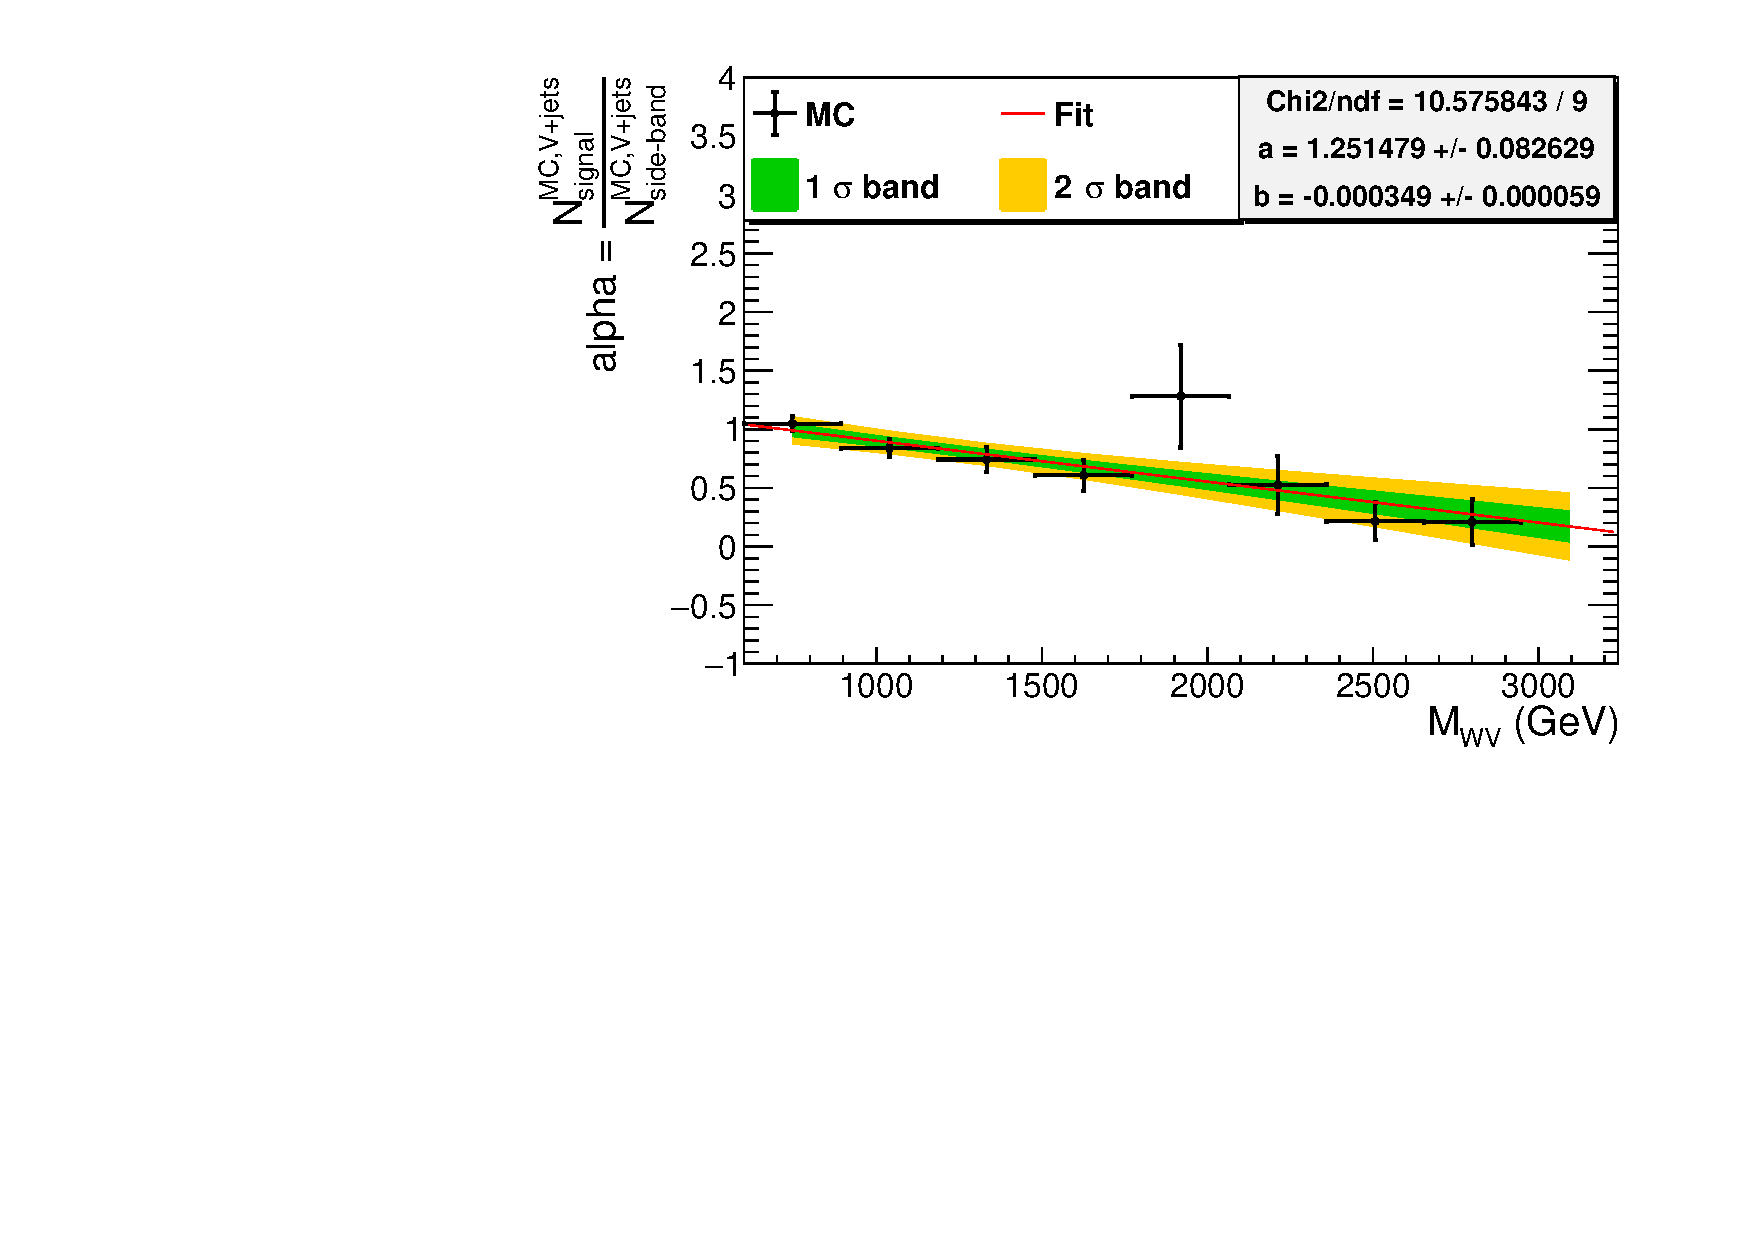
\includegraphics[width=0.68\textwidth]{Plots/BackgroundEstimation/WV/WVchannel_AlphaDistribution_AfterFit_New2.pdf}
	 \caption{Alpha-ratio value (ratios of the $\PW+$jets MC contribution in the signal region to the sideband region) distribution. Red line is the fitted function used in the result.}
	 \label{fig:AlphaDis}
\end{figure}

\begin{figure}[!htbp] 
	 \centering 
	 \begin{subfigure}[b]{0.46\textwidth}
	 	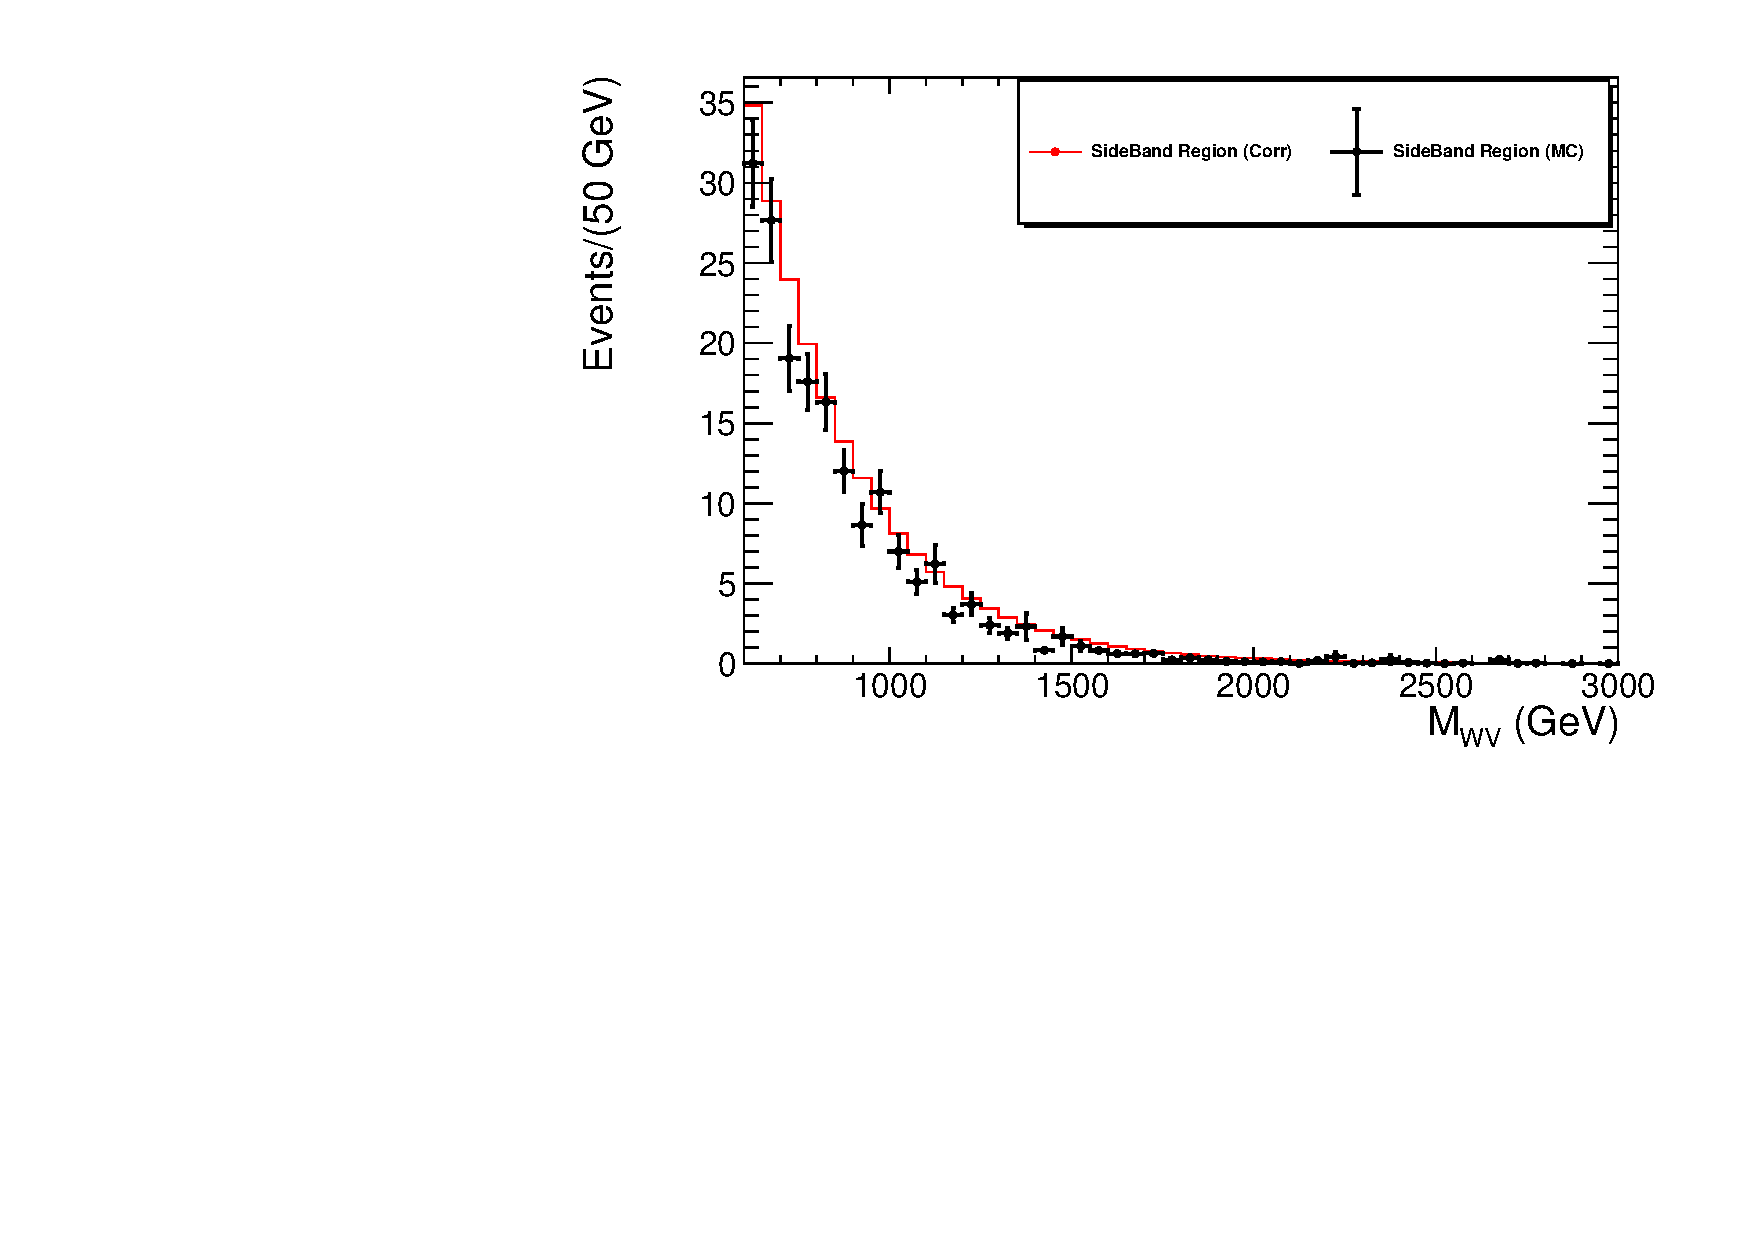
\includegraphics[width=0.9\textwidth]{Plots/BackgroundEstimation/WV/WVchannel_SideBandRegionComparison_VjetShape_MC_CorrShapeFromData.pdf}\qquad
        \caption{ }
        \label{fig:Foil_and_Cone_a}
    \end{subfigure}
	 \begin{subfigure}[b]{0.46\textwidth}
	 	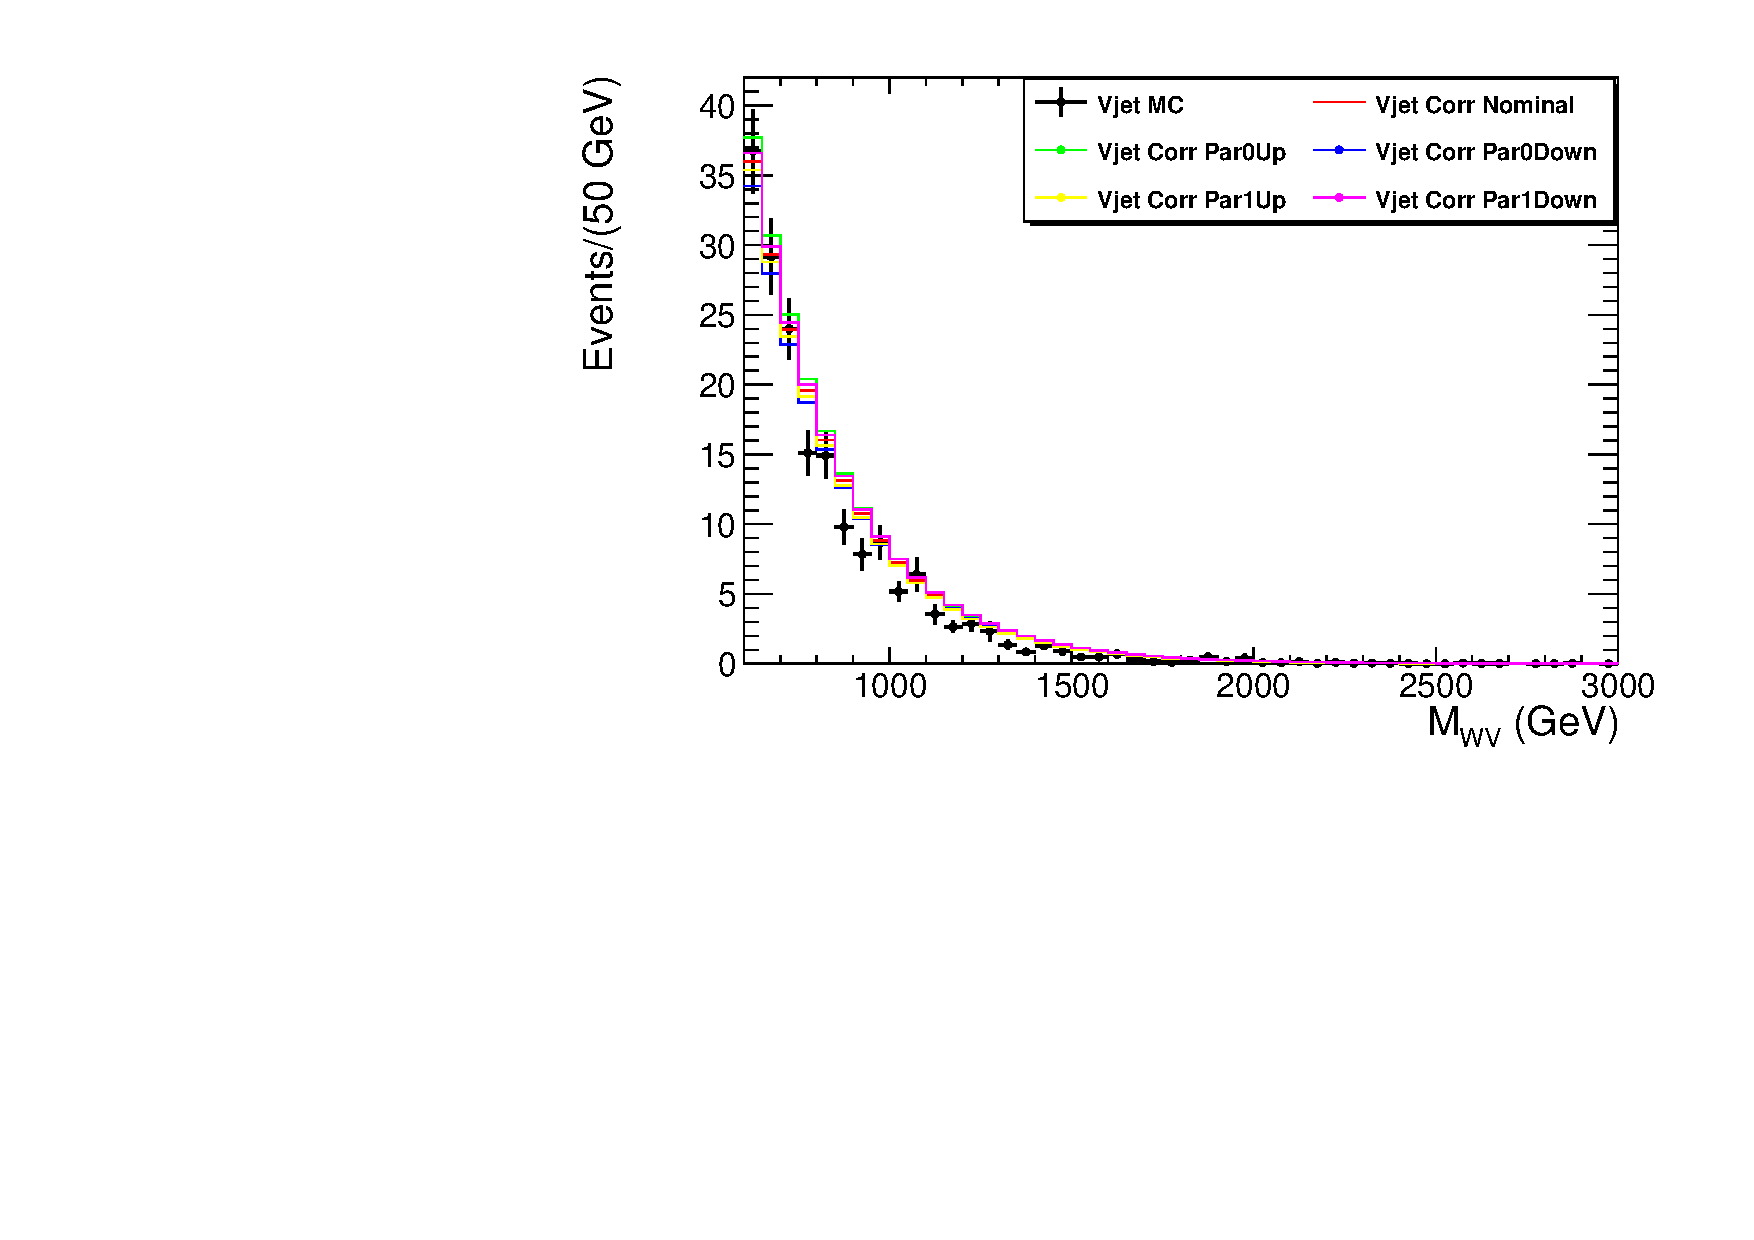
\includegraphics[width=0.9\textwidth]{Plots/BackgroundEstimation/WV/WVchannel_SignalRegionComparison_VjetShape_MC_CorrShapeFromData.pdf}\qquad
        \caption{ }
        \label{fig:Foil_and_Cone_a1}
    \end{subfigure}
	 \caption{Comparison of the $\PW+$jets predictions using simulation (red) and the data-driven estimation in the sideband (left) and signal regions (right). The uncertainty band shows the fit uncertainty.}
	 \label{fig:signal}
\end{figure}
% \begin{figure}[h!]\ContinuedFloat
% 	 \centering 
% 	 \subfigure[]{\includegraphics[width=0.48\textwidth]{Plots/BackgroundEstimation/Wjet_SignalRegion_Nom_up_Down.png}}
% 	 \caption{}
% 	 \label{fig:WjetSignalRegionComp}
% \end{figure}

%\begin{figure}[htbp] 
%	 \centering 
%	 \begin{tabular}{cc}
%	 \includegraphics[width=0.48\textwidth]{Plots/BackgroundEstimation/WV/m_lvj_fitting/m_lvj_sb_lo_WJets0_xww__with_pull.pdf}
%	 \includegraphics[width=0.48\textwidth]{Plots/BackgroundEstimation/WV/m_lvj_fitting/m_lvj_sb_lo_WJets01_xww__with_pull.pdf}\\
%	 \includegraphics[width=0.48\textwidth]{Plots/BackgroundEstimation/WV/DibosonBoostedElMuCuts13TeV_WjetControlRegion_Tighter_CHS_mass_lvj_type0_PuppiAK8_SBR.pdf}
%	 \includegraphics[width=0.48\textwidth]{Plots/BackgroundEstimation/WV/Cross_Check_DataMC_WithWjet_Corr.pdf}
%	 \end{tabular}
%	 \caption{Top: Both distribution are with corrected shape and normalization for W+Jets and other backgrounds shape are taken from fit function fitted to MC. Bottom (left): All backgrounds are taken from MC. Bottom (right): W+jet shape and normalization is taken after correction from data while all other backgrounds are taken from MC.}
%	 \label{fig:DataMCForMWW}
%\end{figure}

The statistical uncertainties from the fits in the sideband region are propagated to the final prediction. The statistical uncertainty in the alpha-ratio values due to limited number of simulated events are also propagated to the result. The $\PW+$jets prediction is also performed with an alternative function as shown above (Figure~\ref{fig:DataMCForMWW}) and the difference from the nominal prediction is taken as a systematic uncertainty.    

The normalization of the $\PW+$jets background in the sideband region is cross-checked by performing a fit to the $m_{V}$ distribution, excluding the signal region. The following parametric functions are used: 

\begin{description}
	\item [V+jets] $f_{User1} = \Big(1-\frac{x}{500}\Big)^p_0/\Big(\frac{x}{500}\Big)^p_1$ 
	\item [V+jets (alternative function)] $f_{ErfExp} = e^{(cx)}. \frac{1}{2}.\Big(1+Erf\big(\frac{x-offset}{width}\big)\Big)$
	\item [TTbar] $f_{2Gaus\_ErfExp} = f_1 \times \Big[e^{(cx)}. \frac{1}{2}.\Big(1+Erf\big(\frac{x-offset}{width}\big)\Big)\Big] + f_2 \times Gaus(x,\mu_1,\sigma_1) + f_3\times Gaus(x,\mu_2,\sigma_2) $
	\item [Single Top, Diboson] $f_{ExpGaus} = f_1 \times e^{(cx)} + Gaus(x,\mu,\sigma) $
\end{description}

The resulting shapes are shown in Figure~\ref{fig:mW_1}. The shown error band is determined by evaluating the fitted functions many times for several points along the x axis with the fitted parameters randomized according to their resulting uncertainties. The extracted fit parameters are summarized in Table~\ref{Table:BackgroundEst_fitPars}. These templates are then used to fit the $m_{V}$ distribution, excluding the signal region. The normalization and shape of the  $\PW$+jets process is floated in the fit. The other background processes are fixed to the SM predictions. The resulting fit is shown in Figure~\ref{fig:Wjet_SR_SBR_Comp}. The resulting normalization of the $\PW+$jets distribution agrees with the normalization obtained from the $m_{WV}$ fit.
\begin{figure}[!htbp] 
	 \centering 
	 \begin{tabular}{c}
	 \includegraphics[width=0.45\textwidth]{Plots/BackgroundEstimation/WV/m_j_fitting/_STop_xwwWWTree_STop_ExpGaus_with_pull.pdf}%
	 \includegraphics[width=0.45\textwidth]{Plots/BackgroundEstimation/WV/m_j_fitting/_TTbar_xwwWWTree_TTbar_2Gaus_ErfExp_with_pull.pdf}\\
	 \includegraphics[width=0.45\textwidth]{Plots/BackgroundEstimation/WV/m_j_fitting/_WJets01_xwwWWTree_VJets_ErfExp_with_pull.pdf}%
	 \includegraphics[width=0.45\textwidth]{Plots/BackgroundEstimation/WV/m_j_fitting/_WJets0_xwwWWTree_VJets_User1_with_pull.pdf}\\
	 \includegraphics[width=0.45\textwidth]{Plots/BackgroundEstimation/WV/m_j_fitting/_VV_xwwWWTree_VV_EWK_QCD_ExpGaus_with_pull.pdf}\\
	 %\includegraphics[width=0.45\textwidth]{Plots/BackgroundEstimation/m_j_fitting/m_j_sideband_WJets01_xww__with_pull.png}
	 \end{tabular}
	 \caption{MC fit distribution for $m_{V}$. Top Left: Single top, Top right: TTbar, Middle left: Wjets with $f_{ErfExp}$, Middle right: Wjets with $f_{User1}$, Bottom: Diboson distribution }
	 \label{fig:mW_1}
\end{figure}
% 1) 0xfc21990 RooRealVar::
\begin{table}[!htbp]
	\centering
	\begin{tabular}{||c | c||} 
	 \hline
	  parameter & Values \\
	 \hline \hline
	 \multicolumn{2}{|c|}{W+jets ($f_{User1}$)}\\
	 \hline
	 $p_0$		&	25.048 $\pm$ 0.885\\
	 $p_1$		&	-4.038 $\pm$ 0.329\\
	 $N$		&	478.191 $\pm$ 35.422\\
	 \hline \hline
	 \multicolumn{2}{|c|}{W+jets (alternate function, $f_{ErfExp}$)}\\
	 \hline
	 c 			&	-0.023 $\pm$ 0.002\\
	 offset 	&	50.918 $\pm$ 2.560\\
	 width 		&	13.742 $\pm$ 3.896\\
	 $N$		&	460.073 $\pm$ 34.228\\
	 \hline \hline
	 \multicolumn{2}{|c|}{Diboson, $f_{ExpGaus}$}\\
	 \hline 
	 $f_1$		&	0.452 $\pm$ 0.018\\
	 c 			&	-0.006 $\pm$ 0.001 \\
	 $\mu$		&	82.313 $\pm$ 0.393\\
	 $\sigma$	&	10.0 $\pm$ 9.412e-07\\
	 $N$		&	87.215 $\pm$ 1.897\\
	 \hline \hline
	 \multicolumn{2}{|c|}{TTbar, $f_{2Gaus\_ErfExp}$}\\
	 \hline 
	 $f_1$		&	0.321 $\pm$ 0.089\\
	 c 			&	-0.025 $\pm$ 0.007\\
	 offset 	&	79.350 (constant)\\
	 width 		&	30.123 $\pm$ 5.731\\
	 $f_2$		&	0.671 (constant)\\
	 $\mu_1$	&	82.789 $\pm$ 0.609\\
	 $\sigma_1$	&	8.520 $\pm$ 0.780\\
	 $f_3$		&	1.0 (constant)\\
	 $\mu_2$	&	$\mu_1$ + 6.913 \\
	 $\sigma_2$	&	$\sigma_1$ + 3.682\\
	 $N$		&	152.598 $\pm$ 4.804\\
	 \hline \hline
	 \multicolumn{2}{|c|}{Single-Top, $f_{ExpGaus}$}\\
	 \hline 
	 $f_1$		&	0.471 $\pm$ 0.081\\
	 c 			&	-0.004 $\pm$ 0.005 \\
	 $\mu$		&	82.602 $\pm$ 1.165\\
	 $\sigma$	&	8.259 $\pm$ 1.019\\
	 $N$		&	35.575 $\pm$ 2.987\\
	 \hline 
	\end{tabular}
 	\caption{Extracted fit parameters for the functions describing the $m_{V}$ distributions.}
 	\label{Table:BackgroundEst_fitPars}
\end{table}
\begin{figure}[!htbp] 
	 \centering 
	 \begin{tabular}{cc}
	 \includegraphics[width=0.48\textwidth]{Plots/BackgroundEstimation/WV/m_j_fitting/m_j_sideband_WJets0_xww__with_pull.pdf}
	 \end{tabular}
	 \caption{Result of the normalization fit in the $m_{V}$ spectrum.}
	 \label{fig:Wjet_SR_SBR_Comp}
\end{figure}

The background estimation is validated using a reduced sideband region and then checking the data-prediction agreement in the  $105~\GeV<~m_{WV}<125~\GeV$ sideband region. The contribution of the $\PW+$jets process is estimated in $105~\GeV<~m_{WV}<125~\GeV$ sideband region by repeating the background estimation above using a reduced sideband region given by requiring $40~\GeV < m_{V} < 65~\GeV$ or $125~\GeV < m_{V} < 150~\GeV$. Figure~\ref{fig:closure} shows (left) that the prediction of the background processes in $105~\GeV<~m_{WV}<125~\GeV$ sideband region is in good agreement with the data. For comparison, the predictions taken from simulation are also shown (right). 

\begin{figure}[!htbp] 
	 \centering 
	 \begin{tabular}{cc}
	 \includegraphics[width=0.48\textwidth]{Plots/BackgroundEstimation/WV/signal_region_Closure_test_AfterCorrShape_38bins.pdf}
         \includegraphics[width=0.48\textwidth]{Plots/BackgroundEstimation/WV/DibosonBoostedElMuCuts13TeV_WjetControlRegion_Tighter_CHS_mass_lvj_type0_PuppiAK8_ClosureTest_SignalRegion.png}  
	 \end{tabular}
	 \caption{The data and predicted $m_{WV}$ distribution obtained from the alpha-ratio method (left) and simulation (right).}
	 \label{fig:closure}
\end{figure}


\subsection{$\PZ+$jets}
The $\PZ+$jets background process prediction in the $\PZ V$ final state is performed using the alpha-ratio method descriped above. The methods to obtain the prediction and the corresponding systematic uncertainties are identical to what was done for the $\PW+$jets prediction in the $\PW V$ final state. Figure~\ref{fig:zvfits} shows the corresponding fit of the $m_{ZV}$ distribution in the sideband region in the $\PZ V$ final state.  

\begin{figure}[!htbp] 
	 \centering 
	 \begin{tabular}{cc}
	 \includegraphics[width=0.48\textwidth]{Plots/BackgroundEstimation/ZV/m_lvj_fitting/m_lvj_sb_lo_WJets0_xww__with_pull.pdf}
	 \includegraphics[width=0.48\textwidth,height=5.5cm]{Plots/BackgroundEstimation/ZV/ZVchannel_AlphaDistribution_AfterFit_New2.pdf}
	 \end{tabular}
	 \caption{The data distribution and the corresponding fit of the $m_{ZV}$ distribution in the sideband region (left) and alpha-ratio value distribution (right).}
	 \label{fig:zvfits}
\end{figure}

% section background_estimation (end)


\section{Systematic Uncertanity} % (fold)
\label{sec:systematic_uncertanity}
In the following the systematic uncertainties which are taken into account in the fit to the $m_{WV}$ and $m_{ZV}$ shapes are listed.  
Uncertainties which do not only influence the overall normalization (\eg the uncertainty in the luminosity measurement), but also the distribution of relevant kinematic observables (\eg the uncertainty in the jet energy scale), are treated as shape uncertainties.
The shape variation is included in the combine tool by providing the histogram templates shifted up and down by one standard deviation.
For each source of uncertainty, the impact in different bins of the final distribution is thus considered fully correlated, while independent sources of uncertainty are treated as uncorrelated. 

%%%%%%%%%%%%%%%%%%%%%%%%%%%%%%%%%%
\subsection{Luminosity}
%%%%%%%%%%%%%%%%%%%%%%%%%%%%%%%%%%

The assigned uncertainty to the integrated luminosity measurement for
the data set used in this analysis is 2.5\%.

%%%%%%%%%%%%%%%%%%%%%%%%%%%%%%%%%%
\subsection{Trigger, lepton reconstruction and identification efficiencies}
%%%%%%%%%%%%%%%%%%%%%%%%%%%%%%%%%%

Discrepancies in the lepton reconstruction and identification
efficiencies between data and simulation are corrected by applying
to all MC samples 
data-to-simulation scale factors measured using $\dyll$ events in the $\cPZ$
peak region~\cite{Tag_probe} that are recorded with unbiased triggers. These factors
depend on the lepton \pt and $\eta$ and are within 1-2\% for electrons and muons.
The uncertainty in the determination of the trigger efficiency leads to an uncertainty smaller than 1\% in the expected signal yield. 

% %%%%%%%%%%%%%%%%%%%%%%%%%%%%%%%%%%
% \subsection{Lepton momentum scale}
% %%%%%%%%%%%%%%%%%%%%%%%%%%%%%%%%%%

% The lepton momentum scale uncertainty is computed by varying the
% momentum of the leptons by their uncertainties. We have an 
% uncertainty in the muons and electrons of 1\%. 
% We follow the recommendations of the Exotica group for the high $p_{T}$ muons~\cite{Twiki:EXO-MUODocumentationRun2}.

%%%%%%%%%%%%%%%%%%%%%%%%%%%%%%%%%%
\subsection{Jet energy scale and resolution}
%%%%%%%%%%%%%%%%%%%%%%%%%%%%%%%%%%

The uncertainty in the calibration of the jet energy scale (JES) and resolution (JER)~\cite{Collaboration2011} 
directly affects the acceptance of the requirement $< 2$~jets, 
the $\met$ computation, and all the cuts related to jets. 
The estimate of the jet energy scale uncertainty is performed varying 
the jet energy scale up and down by 1$\sigma$~\cite{twiki:JES}. The variation
corresponds to a simple re-scaling of the jet four-momentum as
follows: $P\rightarrow P \cdot (1 \pm \delta\pt^{JES}/{\pt})$, where 
$\delta\pt^{JES}$ is the absolute uncertainty on the jet energy scale
which is parametrized as function of the $\pt$ and $\eta$ of the jet. 

A similar strategy is performed to evaluate the systematic related to
the jet energy resolution. In order to reproduce in MC the jet
resolution measured in data the momentum of jets used in this 
analysis is smeared as 
%%
\begin{equation}
p_{\rm T} \rightarrow \max \left[0 , p_{T}^{\rm gen} + c_{\pm1\sigma}\cdot (p_{\rm T}-p_{\rm T}^{\rm gen}) \right]
\end{equation}
%%
in which $c_{\pm1\sigma}$ are the data-to-MC scale factors 
shifting the central value by $\pm$1$\sigma$~\cite{twiki:JES}. 
% These values are taken 
% from the official CMS recommendations for 2016~\cite{twiki:JES}.

%%%%%%%%%%%%%%%%%%%%%%%%%%%%%%%%%%
% \subsection{B-tagging efficiency}
%%%%%%%%%%%%%%%%%%%%%%%%%%%%%%%%%%

% In this analysis the b-tagging is used to reject events with real b-jets in the final state since the signal events have little b-jet content.
% The recipe provided by the BTV group using the recommended measurements has been used to both reweight the b-tagging (in)efficiencies of the selected jets and to estimate 
% the associated uncertainties.

%%%%%%%%%%%%%%%%%%%%%%%%%%%%%%%%%%
\subsection{V tagging efficiency}
%%%%%%%%%%%%%%%%%%%%%%%%%%%%%%%%%%

For the processes estimated from simulation, the uncertainty in the efficiency of the V tagging requirements is estimated to be $8\%$ in the signal region~\cite{jettagging}. The signal region is defined by requiring $\tau_{21}<0.55$ and $ 65 ~\GeV < m_{V} < 105 ~\GeV$. 

%%%%%%%%%%%%%%%%%%%%%%%%%%%%%%%%%%
\subsection{Pileup}
%%%%%%%%%%%%%%%%%%%%%%%%%%%%%%%%%%

MC samples are re-weighted with 69.2 mb as MinBias cross section to reproduce the pileup conditions observed in data.
To compute the uncertainty related to this re-weighting procedure, we
shift the mean of the distribution of real interaction in MC by the
suggested value~\cite{twiki:Pileup} of 5\%. 
The variation of the final yields induced by
this procedure is about 5\% in MC estimated processes. 


%%%%%%%%%%%%%%%%%%%%%%%%%%%%%%%%%%
\subsection{MC statistics}
%%%%%%%%%%%%%%%%%%%%%%%%%%%%%%%%%%

For the processes estimated from simulation, the
available statistics of the MC sample limits the precision of the
modeling, and is therefore taken as a systematic
uncertainty. Similarly, the backgrounds estimated from data are
limited by the available statistics in the corresponding control
samples. Therefore, for these uncertainties, the same treatment is
used as in the case of MC-driven backgrounds.

%%%%%%%%%%%%%%%%%%%%%%%%%%%%%%%%%%
\subsection{Theoretical uncertainties}
%%%%%%%%%%%%%%%%%%%%%%%%%%%%%%%%%%
The predictions of the SM EW and QCD diboson background, and aQGC/Higgs signal processes are taken from simulation. The theoretical Uncertainties in the normalization are derived from variations of the QCD scale, $\alpha_{s}$
and parton distribution functions (PDFs) variations~\cite{Botje:2011sn,Alekhin:2011sk,Lai:2010vv,Martin2009,Ball:2011mu}.
The PDF and $\alpha_s$ uncertainties for signal and background processes are estimated from the standard deviation of weights from the replicas provided in the NNPDF3.0 parton distribution set~\cite{nnpdf}. The procedure for estimating uncertainties arising from Parton Distribution Functions (PDF uncertainties) follows the recommendations as described in paper \textit{``PDF4LHC recommendations for LHC Run II''}~\cite{Butterworth2015}.

Figure~\ref{fig:theory} shows the nominal and the up/down one standard deviation predictions for the QCD scale (left) and PDF uncertainties (right) for the SM EW (top) and SM QCD (bottom) diboson background predictions. The QCD scale uncertainties are  up to ~20\% for the signal normalization (depending on the kinematic region) and 40\% for the QCD initiated diboson background normalization. The uncertainty in the PDF results in up to 10\% variation for the signal and background normalization.
%
\begin{figure}[!htbp]
  \begin{center}
    \includegraphics[width=0.45\textwidth]{Plots/systematic/diboson_QCDScale.pdf}
    \includegraphics[width=0.45\textwidth]{Plots/systematic/diboson_PDFScale.pdf}
    \includegraphics[width=0.45\textwidth]{Plots/systematic/VVjjQCD_QCDScale.pdf}
    \includegraphics[width=0.45\textwidth]{Plots/systematic/VVjjQCD_PDFScale.pdf}
    \caption{Nominal and up/down one standard deviation predictions for the SM EW (top) and SM QCD (bottom) background processes showing the effects of the QCD scale (left) and PDF (right) uncertainties.}
    \label{fig:theory}
  \end{center}
\end{figure}

%%%%%%%%%%%%%%%%%%%%%%%%%%%%%%%%%%
\subsection{$V+$jets}
%%%%%%%%%%%%%%%%%%%%%%%%%%%%%%%%%%
The statistical uncertainties from the fit in the sideband region are propagated to the final prediction. The fit normalization uncertainty is $15\%$. The fit function is modeled using a functional shape of form $f=\exp\left[-m/(c_{0}+c_1\cdot m)\right]$ in the control region fit. The uncertainties in the fit parameters - $c_{0}$ and $c_{1}$ - are treated as nuisance parameters in the combine fit and affect the shape of the background prediction. Figure~\ref{fig:wjet} shows the nominal and the up/down one standard deviation predictions. The statistical uncertainty in the alpha-ratio values due to limited number of simulated events are also propagated to the result. 
%
\begin{figure}[!htbp]
  \begin{center}
    \begin{tabular}{c}
    % \includegraphics[width=0.45\textwidth]{Plots/systematic/WjetFitSyst_Par0_Wjets.png}\\
    \includegraphics[width=0.45\textwidth]{Plots/systematic/WjetFitSyst_Par0_Wjets.pdf}%
    % \includegraphics[width=0.45\textwidth]{Plots/systematic/WjetFitSyst_Par1_Wjets.png}%
    \includegraphics[width=0.45\textwidth]{Plots/systematic/WjetFitSyst_Par1_Wjets.pdf}%
    \end{tabular}
    \caption{Nominal and up/down one standard deviation predictions of the $V+$jets processes for the $c_{1}$ (left) and $c_{0}$ (right) fit parameters.}
    \label{fig:wjet}
  \end{center}
\end{figure}

The $\PV+$jets  prediction is also performed with an alternative function ($f=\exp\left[-m/c_{0}\right]$). The prediction obtained with this function is well within the uncertainties of the nominal prediction as shown in Figure~\ref{fig:wjet2}. For completeness, the difference from the nominal prediction is symmetrized and taken as a systematic uncertainty. The impact of this uncertainty is negligible (see Figure~\ref{fig:pulls} where this uncertainty ranks $18$).    

\begin{figure}[!htbp]
  \begin{center}
    \begin{tabular}{c}
    % \includegraphics[width=0.45\textwidth]{Plots/systematic/WjetFitSyst_Par0_Wjets.png}\\
    \includegraphics[width=0.45\textwidth]{Plots/systematic/WjetFit_all_log.pdf}%
    % \includegraphics[width=0.45\textwidth]{Plots/systematic/WjetFitSyst_Par1_Wjets.png}%
    \includegraphics[width=0.45\textwidth]{Plots/systematic/WjetFitSyst_AlternateShape_Wjets.pdf}%
    \end{tabular}
    \caption{Predictions of the $V+$jets processes for the $f=\exp\left[-m/c_{0}\right]$ functions compared to the nominal prediction (left). The fit uncertainties with this functions are also shown (right).}
    \label{fig:wjet2}
  \end{center}
\end{figure}


%%%%%%%%%%%%%%%%%%%%%%%%%%%%%%%%%%
\subsection{Top }
%%%%%%%%%%%%%%%%%%%%%%%%%%%%%%%%%%
Simulation is used for estimating this process, as described in Section~\ref{sec:sample_used}. The top background prediction is verified in a top enriched control region where the full signal selection is applied, except the b-tagging requirements are reverted. Normalization uncertainty of $10\%$ is assigned to the top background based on the agreement between data and prediction in the control region. 


%%%%%%%%%%%%%%%%%%%%%%%%%%%%%%%%%%
\subsection{Summary}
%%%%%%%%%%%%%%%%%%%%%%%%%%%%%%%%%%

All of the systematic uncertainties on normalizations are given a log-normal 
distribution. A summary of the relative systematic uncertainties in the estimated signal and background
yields is shown in Table~\ref{tab:HwzSystematics}.
\begin{table*}[!htbp]
  \centering
% \cmsTableResize{\begin{scotch}{lccccc}
\begin{tabular}[!htbp]{lccccc}
\hline
\hline
 Source & Signal & $V$+jets & SM EW  & QCD VV & top   \\

        \hline
Integrated luminosity      & 2.5 &  \NA  &  2.5  &   2.5  & \NA \\
Lepton efficiency          & 1.0-2.0  &  \NA  & 1.0-2.0  &  1.0-2.0  & \NA  \\
Jet momentum scale         & shape  & \NA &  shape  &  shape  & shape	 \\
Lepton momentum scale      & shape  & \NA &  shape  &  shape  & shape	 \\
b tagging                  & 2.0 & \NA &  2.0 &   2.0  & 3.0 	 \\
$V$ tagging                & 8.0 & \NA &  8.0 &  8.0  & \NA 	 \\
QCD scale                  & 20 &  \NA  &  20  &  40  & \NA 	 \\
PDF unc.                   & 15 & \NA &  10  &   10  & \NA	 \\
bkg. normalization         & \NA & 10 &  \NA  &  \NA  &  10 \\
$V$+jets shape              & \NA & shape & \NA & \NA & \NA \\
Jet/MET resolution         & 4.0 & \NA &  3.0  & 2.0  & \NA \\
Pileup modeling            & 5.0 & \NA & 4.0 & 4.0 & \NA \\
Limited MC stat.           & shape & \NA & shape & shape & shape \\
\hline
\end{tabular}
\caption{Relative systematic uncertainties in the estimated signal and background yields in units of percent.\label{tab:HwzSystematics}}
\end{table*}
\begin{figure}[!htbp]
\centering
\includegraphics[width=0.7\textwidth]{Plots/plots/impacts_datacard.pdf}
\caption{Impacts and pulls of the systematic uncertainties for the Asimov dataset in the $\PW V$ final state. The impacts are shown for a doubly charged Higgs with a mass of $2000\GeV$.  
}
\label{fig:pulls}
\end{figure}
The pulls and impacts of the systematic uncertainties for the Asimov dataset are shown in Figure~\ref{fig:pulls} in the  $\PW V$ final state. The signal used in the fit is a doubly charged Higgs with a mass of $2000\GeV$. The main experimental systematic uncertainties are related to the uncertainties in the $\PW$+jets background estimation, uncertainties in the jet energy scale and resolution, and  the uncertainty in the efficiency of the $V$ tagging requirements. 



% section systematic_uncertanity (end)


\section{Results} % (fold)
\label{sec:results}
The events in the signal region are used to constrain aQGCs in the effective field theory framework. Nine independent charge conjugate and parity-conserving dimension-8 effective operators are considered~\cite{aqgc_operators}. The dimension-8 operators are the following: 
%
\begin{align*}
L_{S,0} &= \left[\left(D_{\mu} \Phi\right)^{\dagger} D_{\nu} \Phi \right] \times \left[\left(D_{\mu} \Phi\right)^{\dagger} D_{\nu} \Phi \right] \\
L_{S,1} &= \left[\left(D_{\mu} \Phi\right)^{\dagger} D^{\mu} \Phi \right] \times \left[\left(D_{\nu} \Phi\right)^{\dagger} D_{\nu} \Phi \right] \\
L_{M,0} &= Tr[\hat{W}_{\mu \nu} \hat{W}^{\mu \nu}] \times \left[ \left(D_{\beta} \Phi\right)^{\dagger} D^{\beta} \Phi \right] \\
L_{M,1} &= Tr[\hat{W}_{\mu \nu} \hat{W}^{\nu \beta}] \times \left[ \left(D_{\beta} \Phi\right)^{\dagger} D^{\mu} \Phi \right] \\
L_{M,6} &= \left[\left(D_{\mu} \Phi\right)^{\dagger}  \hat{W}_{\beta \nu} \hat{W}^{\beta \nu}  D^{\mu} \Phi \right] \\
L_{M,7} &= \left[\left(D_{\mu} \Phi\right)^{\dagger} \hat{W}_{\beta \nu} \hat{W}^{\beta \mu} D^{\nu} \Phi \right ] \\
L_{T,0} &= Tr \left[W_{\mu \nu} W^{\mu \nu} \right] \times Tr \left[W_{\alpha \beta} W^{\alpha \beta} \right] \\
L_{T,1} &= Tr \left[W_{\alpha \nu} W^{\mu \beta} \right] \times Tr \left[W_{\mu \beta} W^{\alpha \nu} \right] \\
L_{T,2} &= Tr \left[W_{\alpha \mu} W^{\mu \beta} \right] \times Tr \left[W_{\beta \nu} W^{\nu \alpha} \right]
\end{align*}
%
Each operator is scaled by the corresponding Wilson coefficient. A non-zero aQGC enhances the production cross section at large masses of the system of the gauge boson pair as can be seen in Figure~\ref{fig:signal2}. Statistical analysis of the event yields is performed with a fit to the mass distribution of the $\PW V$ or $\PZ V$ system. The SM EW production is treated as a background in the statistical analysis. The observed and expected $95\%$ confidence level (C.L.) limits on the aQGC parameters are obtained using a profile likelihood test statistic~\cite{Junk,Read,Cowan2011}. 

The expected yields for different values of the aQGC parameters are obtained using the reweighting feature of the MadGraph package. The expected ratio of the aQGC and MS EW yields as a function of the aQGC parameter is fitted with a parabolic function. This is done for each bin of the mass distribution of the $\PW V$ or $\PZ V$ system as shown in Figure~\ref{fig:aqgc_pol}. The increase of the yield as a function of the anomalous coupling exhibits a quadratic behaviour and the fitted parabolic function is used to interpolate amongst the discrete coupling parameters of the simulated signals.      

\begin{figure*}[!htbp]
\centering
\includegraphics[width=0.45\textwidth]{Plots/plots/aqgc_pol2.pdf}
\includegraphics[width=0.45\textwidth]{Plots/plots/aqgc_pol2_bin.pdf}
\caption{Yield ratios of the operator $S0$ and the fitted quadratic interpolation for the most relevant bins used in the statistical analysis. The yields for the mass bins $m_{\PW V}$ = [$2025$,$\infty$] (left) and  $m_{\PW V}$ = [$1550$,$2025$] (right) are shown.}
\label{fig:aqgc_pol}
\end{figure*}

Table~\ref{tab:VBS_aQGC} shows the individual lower and upper limits obtained by setting all other aQGCs to zero using the $\PW V$ final state. The reported values are the most stringent limits reported by the CMS Collaboration previously. The corresponding limits using the $\PZ V$ final state are shown in Table~\ref{tab:VBS_aQGC2}. The combined limits are shown in Table~\ref{tab:VBS_aQGC3}.

\begin{table}[!htbp]
\centering
\begin{tabular}{ccc}
\hline
\hline
& Observed limits  & Expected limits  \\
& (\TeV$^{-4}$)   & (\TeV$^{-4}$)   \\
\hline
$\mathrm{f_{S0}} / \Lambda^4$  & $[ -2.6, 2.7]$ & $[ -4.0, 4.0]$ \\
$\mathrm{f_{S1}} / \Lambda^4$  & $[-3.2, 3.3]$ & $[-4.9, 4.9]$ \\
$\mathrm{f_{M0}} / \Lambda^4$  & $[-0.66, 0.66]$ & $[-0.95, 0.95]$ \\
$\mathrm{f_{M1}} / \Lambda^4$  & $[ -1.9, 2.0]$ & $[ -2.8, 2.8]$ \\
$\mathrm{f_{M6}} / \Lambda^4$  & $[-1.3, 1.3]$ & $[-1.9, 1.9]$ \\
$\mathrm{f_{M7}} / \Lambda^4$  & $[-3.3, 3.2]$ & $[-4.8, 4.8]$ \\
$\mathrm{f_{T0}} / \Lambda^4$  & $[-0.11, 0.10]$ & $[-0.16, 0.15]$ \\
$\mathrm{f_{T1}} / \Lambda^4$  & $[-0.11, 0.12]$ & $[-0.17, 0.17]$ \\
$\mathrm{f_{T2}} / \Lambda^4$  & $[-0.27, 0.27]$ & $[-0.38, 0.38]$ \\
\hline
\end{tabular}
\caption{
Observed and expected 95\% C.L. limits on the coefficients
for higher-order (dimension-8) operators in the effective
field theory Lagrangian in $\PW V$ final state. 
}
\label{tab:VBS_aQGC}
\end{table}


\begin{table}[!htbp]
\centering
\begin{tabular}{ccc}
\hline
\hline
& Observed limits  & Expected limits  \\
& (\TeV$^{-4}$)   & (\TeV$^{-4}$)   \\
\hline
$\mathrm{f_{S0}} / \Lambda^4$  & $[ -37, 37]$ & $[ -29, 29]$ \\
$\mathrm{f_{S1}} / \Lambda^4$  & $[-30, 30]$ & $[-23, 23]$ \\
$\mathrm{f_{M0}} / \Lambda^4$  & $[-6.9, 6.9]$ & $[-5.1, 5.1]$ \\
$\mathrm{f_{M1}} / \Lambda^4$  & $[ -21, 21]$ & $[-15, 15]$ \\
$\mathrm{f_{M6}} / \Lambda^4$  & $[-14, 14]$ & $[-10, 10]$ \\
$\mathrm{f_{M7}} / \Lambda^4$  & $[-33, 33]$ & $[-24, 24]$ \\
$\mathrm{f_{T0}} / \Lambda^4$  & $[-1.3, 1.3]$ & $[-0.95, 0.95]$ \\
$\mathrm{f_{T1}} / \Lambda^4$  & $[-1.4, 1.4]$ & $[-0.98, 0.99]$ \\
$\mathrm{f_{T2}} / \Lambda^4$  & $[-3.1, 3.2]$ & $[-2.3, 2.3]$ \\
\end{tabular}
\caption{
Observed and expected 95\% C.L. limits on the coefficients
for higher-order (dimension-8) operators in the effective
field theory Lagrangian in $\PZ V$ final state. 
}
\label{tab:VBS_aQGC2}
\end{table}

\begin{table}[!htbp]
\centering
\begin{tabular}{ccc}
\hline
\hline
& Observed limits  & Expected limits  \\
& (\TeV$^{-4}$)   & (\TeV$^{-4}$)   \\
\hline
$\mathrm{f_{S0}} / \Lambda^4$  & $[ -2.6, 2.7]$ & $[ -4.0, 4.0]$ \\
$\mathrm{f_{S1}} / \Lambda^4$  & $[-3.2, 3.3]$ & $[-4.9, 4.9]$ \\
$\mathrm{f_{M0}} / \Lambda^4$  & $[-0.66, 0.66]$ & $[-0.95, 0.95]$ \\
$\mathrm{f_{M1}} / \Lambda^4$  & $[ -1.9, 2.0]$ & $[ -2.8, 2.8]$ \\
$\mathrm{f_{M6}} / \Lambda^4$  & $[-1.3, 1.3]$ & $[-1.9, 1.9]$ \\
$\mathrm{f_{M7}} / \Lambda^4$  & $[-3.3, 3.2]$ & $[-4.8, 4.8]$ \\
$\mathrm{f_{T0}} / \Lambda^4$  & $[-0.11, 0.10]$ & $[-0.16, 0.15]$ \\
$\mathrm{f_{T1}} / \Lambda^4$  & $[-0.11, 0.12]$ & $[-0.17, 0.17]$ \\
$\mathrm{f_{T2}} / \Lambda^4$  & $[-0.27, 0.27]$ & $[-0.38, 0.38]$ \\
\end{tabular}
\caption{
Observed and expected 95\% C.L. combined limits on the coefficients
for higher-order (dimension-8) operators in the effective
field theory Lagrangian in $\PW V$ and $\PZ V$ final states. 
}
\label{tab:VBS_aQGC3}
\end{table}

 The exclusion limits on the charged Higgs bosons $\sigma_\mathrm{VBF}(\PHpmpm) \, \mathcal{B}(\PHpmpm\to \PW\PW)$ and \newline $\sigma_\mathrm{VBF}(\PHpm) \, \mathcal{B}(\PHpm\to \PW\Z)$ at 95\% confidence level as functions of $m(\PHpm)$ and $m(\PHpmpm)$, respectively, for the $\PW V$ final state are shown in Fig.~\ref{fig:limits} (top left and right).
 A small intrinsic width for $\PHpmpm$ and $\PHpm$ is assumed. 
 The exclusion limit on the charged Higgs $\sigma_\mathrm{VBF}(\PHpm) \, \mathcal{B}(\PHpm\to \PW\Z)$ at 95\% confidence level as a functions $m(\PHpm)$ for the $\PZ V$ final state is shown in bottom left panel in Fig.~\ref{fig:limits}.
 The Higgs bosons $\PHpm$ and $\PHpmpm$ are degenerate in mass (denoted as $m(5)$) at tree level and transform as a five-plet under the custodial symmetry in the GM model.
 The coupling depends on $m(5)$ and the parameter $s_{\PH}$, where $s_{\PH}^2$ denotes the fraction of the $\W$ boson mass squared generated by the vacuum expectation value of the triplets.
 The combination of the model-independent exclusion limits can be used to constrain the $s_{\PH}$-$m(5)$ plane by using the predicted cross sections at NNLO accuracy in the GM model~\cite{Zaro:2002500}.
 The excluded $s_{\PH}$ values as a function of $m(5)$ are shown in Fig.~\ref{fig:limits} (bottom right).


\begin{figure}[!htbp]
\centering
\includegraphics[width=0.45\textwidth]{Plots/plots/limits_wpwp.pdf}
\includegraphics[width=0.45\textwidth]{Plots/plots/limits_wpz_lnu.pdf}
\includegraphics[width=0.45\textwidth]{Plots/plots/limits_wpz_ll.pdf}
\includegraphics[width=0.45\textwidth]{Plots/plots/limits_model.pdf}
\caption{Expected and observed exclusion limits at 95\% confidence level as functions of $m(\PHpmpm)$ and $m(\PHpm)$ for $\sigma_\mathrm{VBF}(\PHpmpm) \, \mathcal{B}(\PHpmpm\to \PW\PW)$ (top left) and $\sigma_\mathrm{VBF}(\PHpm) \, \mathcal{B}(\PHpm\to \PW\Z)$ in the  $\PW V$ (top right) and $\PZ V$ (bottom left) final states, and on the ratio of vacuum expectation values in the GM model (bottom right). The blue shaded area covers the theoretically not allowed parameter space~\cite{Zaro:2002500}.
}
\label{fig:limits}
\end{figure}

% section results (end)
% chapter anomalous_quartic_gauge_coupling_measurement (end)